\pdfminorversion=4

\documentclass[
  draft,
  fontsize=11pt,
  a4paper,
  twoside,
  german,
  headsepline=true,
  footsepline=false,
  automark,
  headings=normal,
  appendixprefix,
  open=any,
  cleardoublepage=plain,
  abstract=true,
  index=totoc,
  listof=totoc,
  bibliography=totoc,
  BCOR9mm,
]{scrreprt}

\usepackage[ngerman]{babel}
\usepackage[utf8]{inputenc}
\usepackage[]{geometry}	% Seitenraender
\usepackage[final]{graphicx}
\usepackage{acronym}
\usepackage{bibgerm}
\usepackage{calc}
\usepackage{color}
\usepackage{colortbl}
\usepackage{scrpage2}
\usepackage{tabularx}
\usepackage{ngerman}
\usepackage{capt-of}
\usepackage{longtable}
\usepackage{amsmath}
\usepackage{pdfpages}
\usepackage{todonotes}
\usepackage{listings}
\usepackage[rightcaption]{sidecap}

\setkomafont{disposition}{\normalcolor\bfseries}
\lstloadlanguages{[LaTeX]TeX}

% Für schöne Darstellung von Algorithmen
\usepackage{algpseudocode}
\usepackage{algorithm}
\usepackage{algorithmicx}

\graphicspath{{img/},{img-results/}}

\usepackage[plainpages=false,pdfpagelabels]{hyperref}
\usepackage{amssymb}
\usepackage[font=normal]{subcaption}
\usepackage{scrhack}

\usepackage{graphicx}
\usepackage{color}
\usepackage{transparent}

% Times New
\usepackage{newtxtext}
\usepackage{newtxmath}
\usepackage{pifont}

% Overflows und Fehlkerning reduzieren
\usepackage[
        activate={true,nocompatibility},
        final,
        tracking=true,
        kerning=true,
        spacing=true,
        factor=1100,
        stretch=10,
        shrink=10
]{microtype}


\graphicspath{{img/},{img-results/}}

\pagestyle{scrheadings} % Standart Kopf- und Fußzeile
\setkomafont{pageheadfoot}{\small\scshape} % for new Koma Script

% ---------------------------------------------------------------------
%\setcounter{secnumdepth}{2}
%\setcounter{chapter}{-1}
\setcounter{tocdepth}{2}

% ---------------------------------------------------------------------
%\sloppy % weniger Worttrennungen, größere Wortabstände
\fussy % viele Worttrennungen, "schönere" Wortabstände

% ---------------------------------------------------------------------
%\flushbottom % Ausrichtung der Seitenenden jeweils auf
% gleicher Höhe

% ---------------------------------------------------------------------
%\sloppypar % Das hier relaxt die Einstellungen zum Wortabstand
% extrem. Damit ragen keine Worte über den rechten
% Zeilenabstand hinaus. Dafür muß stärker auf
% Wortabstand geachtet werden, der kann dann ziemlich
% groß werden. Man erhält aber keine Meldung mehr
% über underfull boxes.

%Hiermit kann man das gleiche mit weniger Holzhammer erreichen:
%\setlength{\tolerance}{2000} % Strafpunkt für Zeilenumbruch
%\setlength{\emergencystretch}{3pt} % Soweit dürfen einzelne Worte mehr
% auseinandergezogen werden
%\setlength{\hfuzz}{1pt} % Macht den rechten Rand um bis zu 1pt
% flatterig.

% ---------------------------------------------------------------------
%Vermeiden einzelner Zeilen am Ende einer Seite oder oben auf einer neuen Seite
\clubpenalty10000
\widowpenalty10000

% eigene Definitionen
\newcommand{\BigO}[1]{$\mathcal{O}(#1)$}
\newcommand{\mergedcell}[2][l]{\begin{tabular}[#1]{@{}l@{}}#2\end{tabular}}
\newcommand{\cmark}{\ding{51}}
\newcommand{\ccross}{\ding{55}}

\newcolumntype{C}{>{\centering\arraybackslash}X}
\newcolumntype{R}{>{\hsize=0.15\textwidth}X}
\newcolumntype{Y}{>{\flushleft\arraybackslash}X}

\newcommand{\cG}[1]{\cellcolor{Green}#1}
\newcommand{\cY}[1]{\cellcolor{Yellow}#1}
\newcommand{\cR}[1]{\cellcolor{Red}#1}

\ifcolortblfix
\definecolor{Green}{rgb}{0.0 1.0 0.0}
\definecolor{Yellow}{rgb}{1.0 1.0 0.0}
\definecolor{Red}{rgb}{1.0 0.0 0.0}
\definecolor{lightgray}{gray}{0.9}

\newcommand{\oddrowcolors}{\def\eltransparency{0.1}\rowcolors{1}{}{black}}
\newcommand{\evenrowcolors}{\def\eltransparency{0.1}\rowcolors{1}{black}{}}

%% rowcolors fix: This makes the rowcolors boxes transparent, so they won't overwrite hline and vline commands (i.e. table borders)
\def\eltransparency{1.0}
\makeatletter
\def\CT@@do@color{%
  \global\let\CT@do@color\relax
        \@tempdima\wd\z@
        \advance\@tempdima\@tempdimb
        \advance\@tempdima\@tempdimc
        \kern-\@tempdimb
\transparent{\eltransparency}%
        \leaders\vrule
                \hskip\@tempdima\@plus 1fill
        \kern-\@tempdimc
        \hskip-\wd\z@ \@plus -1fill }
\makeatother
%\setlength{\arrayrulewidth}{0.6pt}

\else

\definecolor{Green}{rgb}{0.7 1.0 0.7}
\definecolor{Yellow}{rgb}{1.0 1.0 0.7}
\definecolor{Red}{rgb}{1.0 0.7 0.7}
\definecolor{lightgray}{gray}{0.9}

\newcommand{\oddrowcolors}{\rowcolors{1}{}{lightgray}}
\newcommand{\evenrowcolors}{\rowcolors{1}{lightgray}{}}

\fi

\def\arraystretch{1.1}

%threeparttable textwidth
\renewcommand{\TPTminimum}{\textwidth}

%% avoid the [inline] option of todo
\newcommand{\todoline}[1]{\todo[inline]{#1}{}}
\newcommand{\continuehere}{\todoline{continuehere}{}}

\newcommand{\ignore}[1]{}

\DeclareSIUnit\gpcc{\gram\per\cubic\centi\meter}

%% disable todo
\ifdraft{
  \newcommand{\Si}[2]{\todo{Tippfehler: \\Si statt \\SI}\SI{#1}{#2}}
}{
  \renewcommand{\todoline}[1]{}
  \renewcommand{\todo}[1]{}
}

\newcommand{\qqquad}[0]{\qquad\quad}
\newcommand{\pot}[1]{\texttt{#1}}

\newcommand{\chemlegend}[1]{\begin{minipage}[c]{0.7cm}\includegraphics[width=\textwidth]{#1}\end{minipage}}
\newcommand{\chemlegendce}[1]{\chemlegend{#1}\ce{#1}}

%======================================================================
% Metadaten
%======================================================================
% $Id$
% Original template: Matthias Kupfer
%======================================================================

\newcommand{\dcsubject}{Masterarbeit}
\newcommand{\dctitle}{Atomistische Modellierung und Simulation des Filmwachstums bei Gasphasenabscheidungen}
%% \newcommand{\dctitle}{Modellierung und Simulation von Schichtabscheidungen aus der Gasphase}
\newcommand{\dcsubtitle}{} % Untertitel, falls erforderlich

\newcommand{\dcauthortitle}{B.Sc.}
\newcommand{\dcauthorlastname}{Lorenz}
\newcommand{\dcauthorfirstname}{Erik E.}
\newcommand{\dcauthoremail}{erik.e.lorenz@gmail.com}
\newcommand{\dcdate}{\today}

\newcommand{\dcplace}{Chemnitz} % Ort, kann an der TU meist so bleiben
\newcommand{\dcuni}{Technische Universität \dcplace}
\newcommand{\dcdepart}{Fakultät für Naturwissenschaften} % Fakultätsangabe
\newcommand{\dcinstitute}{Institut für Physik}

\newcommand{\dcinstituteext}{Fraunhofer-Institut für Elektronische Nanosysteme}
\newcommand{\dcdepartext}{Abteilung Back-End of Line} % Fakultätsangabe

\newcommand{\dcexaminerfirst}{Prof. Dr. Stefan E. Schulz}
\newcommand{\dcdepartfirst}{Fakultät für Elektrotechnik und Informationstechnik} % Fakultätsangabe
\newcommand{\dcproffirst}{Technologien der Nanoelektronik} % Angabe der Professur

\newcommand{\dcexaminersecond}{Prof. Dr. Karl Heinz Hoffmann}
\newcommand{\dcdepartsecond}{Fakultät für Physik} % Fakultätsangabe
\newcommand{\dcprofsecond}{Theoretische Physik, insbesondere Computerphysik} % Angabe der Professur
\newcommand{\dcinstitutesecond}{\dcinstitute}

\newcommand{\dcadvisor}{Dr. Jörg Schuster}
\newcommand{\dcinstituteadvisor}{\dcinstituteext}
\newcommand{\dcdepartadvisor}{\dcdepartext}
\newcommand{\dcgroupadvisor}{Simulationsgruppe}

\newcommand{\dckeywords}{Dünne Schichten, chemische Gasphasenabscheidung (CVD), physikalische Gasphasenabscheidung (PVD), Atomlagenabscheidung (ALD), Multiskalenmodellierung, Kinetic Monte Carlo (KMC), Molekulardynamik (MD), ReaxFF}

%%======================================================================
% Einstellungen des Hyperref-Paketes
\hypersetup{%
 pdftitle = {\dctitle}, %
 pdfsubject = {\dcsubject, \dcdate}, %
 pdfauthor = {\dcauthorfirstname~\dcauthorlastname, \dcauthoremail}, %
 pdfkeywords = {\dckeywords}, %
 pdfcreator = {pdfTeX with Hyperref and Thumbpdf}, %
 pdfproducer = {LaTeX, hyperref, thumbpdf}, %
 % weitere pdf-Einstellungen in hyperref.cfg
}
%%======================================================================


\begin{document}

%======================================================================
%  Titelseite
%======================================================================

% Wir setzten hier die Seitennummerierung auf Großrömisch, auch wenn diese
% nicht auf dem "Papier" erscheint. Es dient nur der internen Zählung der
% Seiten im hyperref-Paket, welches für die Seitennummerierung in den pdfs
% zuständig ist. Ohne diesen Trick kommen ein paar sinnlose Warnungen und
% die Seiten-Navigation im Adobe Reader kann durcheinander geraten.
\pagenumbering{Roman}


%%======================================================================
%% Schmutztitel
%%======================================================================
%\extratitle{
%  \usekomafont{disposition}\mdseries
%  \begin{center}
%    \Huge \dcsubject\\[1.5ex]
%    \hrule
%    \vspace*{\fill}
%    
\includegraphics{TUC_deutsch_einzeile_CMYK}
%  \end{center}
%}

%%======================================================================
%% Titelkopf
%%======================================================================
\titlehead{
  \vspace*{-1.5cm}
  \begin{center}
    \raisebox{-1ex}{
\includegraphics[scale=1.1]{img/logo_tu_tailored}}\\
    \hrulefill \\[1em]
    {\Large\dcdepart}\\[0.2em]
    \dcinstitute\\[0.5em]
%    {\Large\dcdepartsecond}\\[0.5em]
%    \dcprofsecond
  \end{center}
  \vspace*{0.1cm}
  \begin{center}
    \raisebox{-1ex}{
\includegraphics[scale=1.2]{img/logo_fhg_tailored}}\\
    \hrulefill \\[1em]
    {\Large\dcinstituteext}\\[0.2em]
    \dcdepartext\\[0.5em]
  \end{center}
  \vspace*{0.5cm}
}



%%======================================================================
%% Subjekt
%%======================================================================
\subject{\huge\textnormal{\textsc{\dcsubject}}}


%%======================================================================
%% Titel
%%======================================================================
\title{\huge
  \dctitle
  \\
  \dcsubtitle
  \vspace*{-0.4em}
}

%%======================================================================
%% Autor des Dokumentes
%%======================================================================
\author{\dcauthortitle~\dcauthorfirstname~\dcauthorlastname}

%%======================================================================
%% Ort, Datum
%%======================================================================
\date{\dcplace, den \dcdate
}


%%======================================================================
%% Publishers
%%======================================================================
\publishers{
    \begin{tabbing}
      \hspace*{10.1em}\=\kill
      \hspace*{4.8em}{Gutachter:}\>\dcexaminerfirst\\[-0.2em]
                  \>{\small\dcproffirst}\\[0.2em]
                  \>\dcexaminersecond\\[-0.2em]
                  \>{\small\dcprofsecond}\\
\\
      \hspace*{4.8em}{Betreuer:}\>\dcadvisor\\[-0.2em]
                  \>{\small\dcinstituteadvisor}
    \end{tabbing}
  \vspace*{-7em}
}

%%======================================================================
%% bibliografische Angaben
%%======================================================================
\lowertitleback{
\textbf{\dcauthorlastname, \dcauthorfirstname}\\
\textit{\dctitle}\\
%\dcsubject,~\dcdepart\\
\dcsubject\\
\dcuni,~\ifcase\month\or
  Januar\or Februar\or März\or April\or Mai\or Juni\or
    Juli\or August\or September\or Oktober\or November\or Dezember\fi
    ~\number\year\\
Stichworte: \dckeywords
}

%%======================================================================
%% maketitle
%%======================================================================

\maketitle

%%======================================================================
%% Danksagung
%%======================================================================
%\thispagestyle{empty}
%\null\vfil
%\begin{center}
%\usekomafont{disposition}\textbf{Danksagung}
%\vspace{-.5em}\vspace{\parsep}
%%
%% Hier steht der Text für die Danksagung
%%
%\end{center}
%\par\vfil\null
%\cleardoubleemptypage

%%======================================================================
%%      Kurzfassung / Abstract
%%======================================================================
%\def\abstractname{Abstract} % Wenn der Text "Zusammenfassung" erscheinen
                             % soll, dann muß dies auskommentiert werden


\pagenumbering{roman}

\begin{abstract}
ASD
\end{abstract}

%%======================================================================
%%      Inhaltsverzeichnis
%%======================================================================
%\clearpage

%\cleardoubleemptypage

%\pdfbookmark{Inhaltsverzeichnis}{Inhaltsverzeichnis}
\tableofcontents

%%======================================================================
%%      Abbildungsverzeichnis
%%======================================================================
%\cleardoublepage
\markboth{Abbildungsverzeichnis}{Abbildungsverzeichnis}
\listoffigures
\todo[inline]{Beschreibungen der Abbildungen überarbeiten}

%%======================================================================
%%      Tabellenverzeichnis
%%======================================================================
%\cleardoublepage
\markboth{Tabellenverzeichnis}{Tabellenverzeichnis}
\listoftables
\todo[inline]{Beschreibungen der Tabellen überarbeiten}

%======================================================================
%  Literaturverzeichnis
%======================================================================
%\cleardoublepage
%\manualmark
%\markboth{Literaturverzeichnis}{Literaturverzeichnis}
%\bibliographystyle{unsrt}
%\bibliographystyle{own}
%\bibliography{literatur}

%%======================================================================
%%      Algorithmenverzeichnis
%%======================================================================
%% \renewcommand{\listalgorithmname}{Algorithmenverzeichnis}
%% \addcontentsline{toc}{chapter}{Algorithmenverzeichnis}
%% \listofalgorithms

%%======================================================================
%%      Abkuerzungsverzeichnis
%%======================================================================
%\cleardoublepage
\chapter*{Abkürzungsverzeichnis}
\addcontentsline{toc}{chapter}{Abkürzungsverzeichnis}
\markboth{Abkürzungsverzeichnis}{Abkürzungsverzeichnis}
\def\listacronymname{Abkürzungsverzeichnis}

\newcolumntype{Y}{>{\flushleft\arraybackslash}X}

%\begin{acronym}[SQL]
% \acro{CNTs}{Kohlenstoffnanoröhrchen (engl. Carbon Nanotubes, CNTs)}
% \acro{DFT}{Dichtefunktionaltheorie}
%\end{acronym}

\def\arraystretch{1.3}
\begin{longtable}{lll}

AFM       & Atomic Force Microscopy             & Rasterkraftmikroskopie                                      \\
ALD       & Atomic Layer Deposition             & Atomlagenabscheidung                                        \\
CG        & Conjugated Gradients                & Konjugierte Gradienten                                      \\
CLI       & Command Line Interface              & Kommandozeile                                               \\
CVD       & Chemical Vapor Deposition           & Chemische Gasphasenabscheidung                              \\
DFT       & Density Functional Theory           & Dichtefunktionaltheorie                                     \\
EAM       & Embedded Atom Method                & Eingebettete-Atom-Methode                                   \\
FEM       & Finite Element Method               & Finite-Elemente-Methoden                                    \\
GMR       & Giant Magnetoresistance             & Riesenmagnetowiderstand                                     \\
GPC       & Growth per Cycle                    & Schichtwachstum pro ALD-Zyklus                              \\
KMC       & Kinetic Monte Carlo                 & Kinetische Monte Carlo-Methoden                             \\
MMC       & Metropolis Monte Carlo              & Metropolis Monte Carlo-Methoden                             \\
MD        & Molecular Dynamics                  & Molekulardynamik                                            \\
MEAM      & Modified Embedded Atom Method       & Modifizierte Eingebettete-Atom-Methode                      \\
MOSFET    & Metal Oxide Field Effect Transistor & Metalloxid-Feldeffekt-Transistor                            \\
MPI       & Message Passing Interface           & Eine Kommunikationsschnittstelle                            \\
NB        & Neighborhood                        & (atomare) Nachbarschaft                                     \\
PVD       & Physical Vapor Deposition           & Physikalische Gasphasenabscheidung                          \\
RAM       & Random-Access Memory                & Arbeitsspeicher                                             \\
RDF       & Radial Distribution Function        & Radiale Verteilungsfunktion                                 \\
RMS       & Root Mean Square                    & Standardabweichung                                          \\
ReaxFF    & Reactive Force Fields               & Reaktive Kraftfelder                                        \\
TMA       & Trimethylaluminum (\ce{Al(CH3)3})   & Trimethylaluminium (\ce{Al(CH3)3})                          \\
NPT       & \multicolumn{2}{l}{Großkanonisches Ensemble: Teilchenzahl, Druck und Temperatur sind konstant}    \\
NVE       & \multicolumn{2}{l}{Mikrokanonisches Ensemble: Teilchenzahl, Volumen und Energie sind konstant}    \\
NVT       & \multicolumn{2}{l}{Kanonisches Ensemble: Teilchenzahl, Volumen und Temperatur sind konstant}      \\
Parsivald & \multicolumn{2}{l}{Parallel Atomistic Reaction Simulator for Vapor and Atomic Layer Depositions}  \\

\end{longtable}

\begin{comment}
  Liste der Abkürzungen, die nicht weiter erklärt werden:
  (Comment-Umgebung, damit sie vom Parser trotzdem erfasst werden)

  ENAS      & \multicolumn{2}{l}{Fraunhofer-Institut für Elektronische Nano-Systeme}                            \\
  LAMMPS    & \multicolumn{2}{l}{Large-scale Atomic/Molecular Massively Parallel Simulator (MD-Bibliothek)}     \\
  AMBER
  GROMACS
  BIOVIA
  TU
  EU
  ACCELERATE
\end{comment}

\todo[inline]{NB vorstellen?}
\todo[inline]{MMC: schönerer Name?}
\todo[inline]{Beschreibung der Ensembles hier oder nur im Text?}
\todo[inline]{Prüfen, ob die Abkürzungen im Text ordentlich eingeführt werden}

\chapter*{Symbolverzeichnis}
\addcontentsline{toc}{chapter}{Symbolverzeichnis}
\markboth{Abkürzungsverzeichnis}{Symbolverzeichnis}
\def\listacronymname{Symbolverzeichnis}

\begin{tabularx}{\linewidth}{ll}
$E_\text{A}$       & Aktivierungsenergie            \\
$p_\text{partial}$ & Partialdruck                   \\
$\sigma_z$         & RMS-Rauheit einer Oberfläche   \\
$\tau$             & Dämpfungszeit von Thermostaten \\
\end{tabularx}
\todo[inline]{die wichtigsten Symbole automatisch aus allen Formeln exportieren}
\todo[inline]{Verweise von Gleichungen durch Lokalität ersetzen}
\todo[inline]{Kein neuer Absatz nach Gleichungen}

%\printglosstex(acr)

%%======================================================================
%%      Ende
%%======================================================================
\cleardoublepage
\pagenumbering{arabic} % Fäng erneut bei 1 an.


\pagenumbering{arabic}

\cleardoublepage
\chapter{Einleitung}
\label{intro}

%% {Aktueller Stand der Technologien und damit verbundene Herausforderungen}
Gasphasenabscheidungen werden zur Herstellung konformer, dünner Schichten auf strukturierten und glatten Substraten genutzt, wobei besonders die Erzeugung ultradünner, hoch reiner, homogener Schichten eine Schlüsselstellung bei der Fertigung von Bauelementen in der Nanoelektronik einnimmt\cite{granneman_thin_1993}.
Sie sind beispielsweise für die Produktion dünner Dielektrika\cite{gordon_vapor_2001}, Interconnects\cite{waechtler_copper_2009} und Diffusionsbarrieren\cite{granneman_thin_1993,raaijmakers_low_1994} interessant, für die besonders präzise Abscheidungsmethoden notwendig sind.
%% {weitere Anwendungen von Gasphasenabscheidung}
Gasphasenabscheidungen werden auch für eine Vielzahl anderer Anwendungen verwendet, wie beispielsweise für die Produktion von passivierenden und protektiven Beschichtungen\cite{yun_passivation_2004,poodt_high-speed_2010,higashiwaki_algan/gan_2006}.
Weiterhin erlauben sie die Herstellung mehrlagiger Materialien mit besonderen mechanischen (erhöhte Festigkeit\cite{cammarata_nanoindentation_1990}), magnetischen (Riesenmagnetowiderstand\cite{peter_influence_2007,seyama_giant_1999,bird_giant_1995}, magnetischer Tunnelwiderstand\cite{sun_magnetic_2006}) und optischen Eigenschaften (Röntgenspiegel\cite{jankowski_subnanometer_1989}).
Doch auch größere Oberflächen werden per Gasphasenabscheidung mit Dünnschichten versehen, etwa zur Erhöhung der Witterungs- und Wärmebeständigkeit von Oberflächen\cite{mccurdy_successful_1999}.

%% {Kandidat zur Lösung von Herausforderungen}
Bei Gasphasenabscheidungen adsorbieren einzelne Atome oder Moleküle aus der Gasphase auf der Oberfläche und bilden so eine dünne Schicht, deren Dicke präzise im Sub-Nanometer-Bereich kontrolliert werden kann\cite{mattox_handbook_2010,pierson_handbook_1999}.
Mit der Physikalischen Gasphasenabscheidung (PVD, Physical Vapor Deposition), der Chemischen Gasphasenabscheidung (CVD, Chemical Vapor Deposition) und der Atomlagenabscheidung (ALD, Atomic Layer Deposition) stehen Methoden zur Verfügung, welche das Wachstum verschiedener Materialien mit unterschiedlichen Graden der Prozesskontrolle erlauben.

%% {Mein Gebiet}
Atomistische Simulationen können helfen, unter verschiedenen Bedingungen die strukturellen Eigenschaften der abgeschiedenen Schicht zu beschreiben, anhand derer auch Rückschlüsse auf elektronische\cite{aspnes_optical_1982,steudel_influence_2004} oder mechanische Eigenschaften\cite{chasiotis_mechanical_2003,cammarata_nanoindentation_1990} gezogen werden können.
Dafür ist eine Modellierung chemischer Reaktionen und amorpher Strukturen ebenso notwendig wie die Beschreibung von Simulationsräumen auf der Größenordnung kompletter Nano-Bauelemente, um ebenfalls Aussagen über das Wachstum auf strukturierten, polykristallinen oder heterogenen Substraten treffen zu können.
Zur Simulation von Abscheidungen auf kompletten Nano-Bauelementen sind große Simulationsräume im Bereich von \SI{200x200}{\nano\meter} mit \num{1e8} Atomen notwendig, die mit rein atomistischen Simulationen bisher aufgrund des hohen Rechenaufwandes nicht möglich sind\cite{plimpton_computational_1995}.
% oder keine strukturellen Aussagen ermöglichen.

%% {Möglichkeiten zur Optimierung}
Ansatzpunkte für die Simulation von Gasphasenabscheidungen bestehen in Kinetischen Monte Carlo-Methoden (KMC)\cite{voter_introduction_2007} einerseits und in der Molekulardynamik (MD)\cite{hoover_molecular_1986} andererseits.
KMC kann die Reaktionskinetik komplizierter Prozesse in großen Simulationsräumen zufriedenstellend beschreiben, ermöglicht allerdings keine detaillierte strukturelle Beschreibung der simulierten Materialien.
MD hingegen simuliert effizient atomistische Strukturen, lässt sich aber nur unzureichend zur Beschreibung von großen Simulationsräumen nutzen.
Mit der Einführung reaktiver Kraftfelder haben molekulardynamische Simulationen zudem die Möglichkeit gewonnen, chemische Reaktionen effizient zu simulieren, doch sind diese rechenaufwendiger als herkömmliche Kraftfelder und erlauben nur die Simulation weniger tausend Atome\cite{van_duin_reaxff:_2001}.
Eine mögliche Lösung dieser Probleme stellt eine Kombination der beiden Methoden dar, durch die atomistische Simulationen von vollständigen Beschichtungen kompletter Nano-Bauelemente ermöglicht werden.

%% {Anknüpfungspunkte und Fokus der Arbeit}

Das Ziel der vorliegenden Arbeit ist, ein bestehendes Multiskalen-Modell zur Simulation von Atomlagenabscheidungen per KMC und MD auf allgemeine Gasphasenabscheidungen zu erweitern und die Simulation von Gasphasenabscheidungen, insbesondere der physikalischen Gasphasenabscheidung, damit zu realisieren.
Dabei soll auch die Präparation neuer Abscheidungsprozesse sowie die Möglichkeit untersucht werden, die Oberflächen-Reaktionen bei chemischen Gasphasenabscheidungen durch reaktive Kraftfelder molekulardynamisch zu beschreiben.
Außerdem soll die vorliegende Implementierung dieses Modelles zugunsten der schnellen Prozesspräparation um Konfigurationsdateien, zentrale Datenbanken der Substrate und Prozesskonfigurationen sowie um eine einfachere Kontrolle der Prozessparallelisierung ergänzt werden.

%% {Struktur der Arbeit}
\subsubsection{Struktur der Arbeit}

Im Anschluss an diese Einleitung wird zuerst in Kapitel~\ref{theory} ein Überblick über die Arten und Funktionsweisen von Gasphasenabscheidungen sowie über die Simulationsmethoden der Molekulardynamik und Kinetischen Monte Carlo-Methoden gegeben.

Danach stellt Kapitel~\ref{models} den aktuellen Stand der Simulationen von Gasphasenabscheidungen mit KMC und MD vor, präsentiert die Erweiterungen des kombinierten KMC/MD-Modells sowie eine Laufzeitanalyse dieses Modells und gibt einen Überblick über allgemeine molekulardynamische Methoden zur Präparation von Prozessen und Substraten sowie über die Analyse von Ergebnissen.

Der Hauptteil der Arbeit beschäftigt sich in Kapitel~\ref{results} mit den Ergebnissen der Simulation von Gasphasenabscheidungen und den notwendigen Voruntersuchungen der molekulardynamischen Potentialparametrisierungen.
Dafür wird zuerst eine Gold-PVD-Simulation als Beispielprozess für nichtreaktive Abscheidungen präpariert und damit das Wachstumsverhalten auf strukturierten Substraten sowie die Skalierbarkeit des kombinierten Modelles überprüft.
Anhand von Kupfer-PVD werden danach Unterschiede zwischen verschiedenen Parametersätzen des selben Kraftfeldes untersucht und die Bildung und Schließung von Oberflächendefekten beobachtet.
Die Simulation gemischter Systeme wird anhand der Multilagen-Abscheidung durch Kupfer-Nickel-PVD untersucht und die entstandenen Strukturen mit den Ergebnissen einer reinen MD-Simulation verglichen.
Anschließend wird die Präparation und Abscheidung amorpher Strukturen am Silizium-PVD-System untersucht.
%, wobei auch Betrachtungen der Gasphasen-Reaktionen für Siliziumoxid-CVD durchgeführt werden.
Zuletzt wird die Hydroxylierung einer Aluminiumoxid-Oberfläche mit Wassermolekülen mit reaktiven Kraftfeldern simuliert.

Zum Abschluss wird die Arbeit mit Kapitel~\ref{summary} zusammen gefasst, bevor zukünftige Fragestellungen und Anknüpfungspunkte für weitere Untersuchungen gegeben werden.

Im Anhang der Arbeit sind experimentelle Referenzwerte, weitergehende Informationen zu den verwendeten Datenstrukturen und dem Laufzeitverhalten von Parsivald sowie ergänzende Ergebnisse der simulierten Gasphasenabscheidungen zu finden.

\cleardoublepage
\cleardoublepage
\chapter{Theorie}

\section{Gasphasenabscheidungen}

Gasphasenabscheidungen sind eine Klasse von Verfahren, bei denen dünne Schichten durch physikalische oder chemische Prozesse aus der Gasphase auf eine Oberfläche aufgetragen werden.
Sie teilen sich in \textbf{Physikalische Gasphasenabscheidung} (PVD, Physical Vapor Deposition), \textbf{Chemische Gasphasenabscheidung} (CVD, Chemical Vapor Deposition) und \textbf{Atomlagenabscheidung} (ALD, Atomic Layer Deposition) auf, die im folgenden betrachtet werden.

Ihnen ist allgemein, dass einzelne Atome oder Moleküle auf der Oberfläche aufkommen, dort physikalisch oder chemisch adsorbiert werden und eventuelle Nebenprodukte aus dem Reaktor gespült werden, wodurch mit vorhersehbarer Rate eine dünne Schicht des Zielmateriales aufwächst.
Tabellen \ref{tab:deposition-comparison} und \ref{tab:deposition-materials} stellen jeweils Charakteristiken und mögliche Materialien für die drei Prozesse dar.

\begin{figure}
  \centering
  \def\svgwidth{\textwidth}
  \input{img/reactors.pdf_tex}
  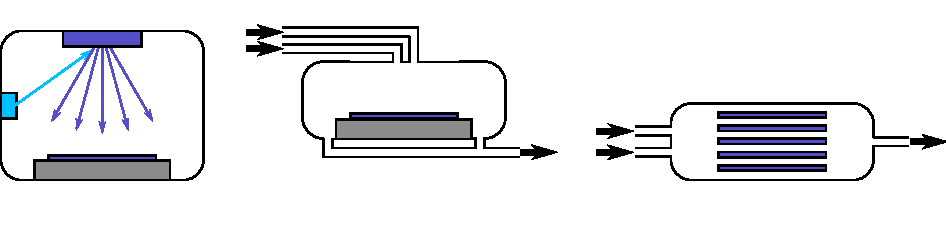
\includegraphics[]{reactors}
  \caption[Abscheidungskammern und -reaktoren]{Abscheidungskammern und -reaktoren}
  \label{fig:reactors}
\end{figure}

\begin{table}
  \centering
  \begin{tabularx}{\textwidth}{|X|ccc|}
    \hline
    Prozesscharakteristiken & \textbf{PVD} & \textbf{CVD} & \textbf{ALD} \\
    \hline
    reaktiv &  & \cmark & \cmark \\
    kontinuierlich & \cmark & \cmark & zyklisch \\
    Gas-Edukte & Atome, Moleküle & Precursor-Moleküle & Precursor-Moleküle \\
    \# Edukte & 1 & 1+ & 2+ \\
    Nebenprodukte & & \cmark & \cmark \\
    Wachstumsrate & $\sim t$ & $\sim t$ & $\sim n_\text{cyc.}$ \\
    \hline
  \end{tabularx}
  \caption[Prozesscharakteristiken der Abscheidungsarten]{Vergleich der Abscheidungsarten}
  \label{tab:deposition-comparison}
\end{table}

\begin{table}
  \centering
  \begin{tabularx}{\textwidth}{XXXXXXXXX}
    & \angled{Metalle} & \angled{Legierungen} & \angled{Metalloxide} & \angled{Nitride} & \angled{Chloride} & \angled{Silizium}  & \angled{Siliziumoxid} & \angled{Diamant} \\
    \hline
    \textbf{PVD} &\cmark&\cmark&&&&\cmark&&?\\
    \textbf{CVD} &\cmark&?&\cmark&\cmark&\cmark&\cmark&?&?\\
    \textbf{ALD} &\cmark&?&\cmark&\cmark&\cmark&\cmark&\cmark&\cmark\\
  \end{tabularx}
  \caption[Mögliche Produkte der Abscheidungsarten]{Mögliche Produkte der Abscheidungsarten. Weitergehende Informationen finden sich in der Literatur für PVD\cite{asd}, CVD\cite{asd} und ALD\cite{puurunen_surface_2005}.}
  \todo[inline]{Referenzen für abgeschiedene Systeme}
  \label{tab:deposition-materials}
\end{table}

\subsection{Physikalische Gasphasenabscheidung}

PVD ist kontinuierlich und nicht reaktiv, arbeitet also mit Atomen oder Molekülen, die physikalisch auf der Oberfläche adsorbieren.
Beispielsweise werden beim Sputtering durch energiereiche Partikel (Argon-Plasma) einzelne Atome aus dem sogenannten Target geschlagen, die dann auf dem Substrat eine homogene, dünne Schicht bilden.
Durch die Nutzung mehrerer Targets (Cosputtering) oder mehrerer Atomsorten in einem Target lassen sich auch Legierungen und andere mehrelementige Materialien abscheiden.
\todo{Referenzen für alles}

\subsection{Chemische Gasphasenabscheidung}

CVD wächst durch chemische Adsorption eines oder mehrerer Precursor-Moleküles eine dünne Schicht auf dem Substrat auf.
Dazu werden die Precursorgase zeitgleich in den Reaktor geleitet, wo sie über die Substratoberfläche strömen und Reaktionen ermöglichen.
Die dabei entstehenden Nebenprodukte werden mit dem Gasstrom aus dem Reaktor geführt, um die aufwachsende Schicht nicht zu verunreinigen.
\todo{zu abrupter Übergang}

Passende Precursor-Kombinationen zu finden, gestaltet sich oft schwierig, da sie idealerweise erst auf der Oberfläche und nicht in der Gasphase reagieren und dabei inerte Nebenprodukte erzeugen sollen.
Weitere Kriterien wie Prozesstemperaturen, Energiebarrieren und komplizierte Reaktionspfade erschweren die Suche zusätzlich.
Im Gegensatz zu PVD kann CVD dafür auf allen Substraten, über deren Oberfläche ein kontinuierlicher Gasfluss möglich ist, eine dünne Schicht abscheiden.
Dies beinhaltet Stufen, Rillen und anderweitig strukturierte Substrate ebenso wie Poren durch das Substrat.

\missingfigure{Beispiel Precursor-Moleküle}

\subsection{Atomlagenabscheidung}

\begin{figure}
  \centering
  \def\svgwidth{\textwidth}
  \input{img/ald-schema.pdf_tex}
  \caption[ALD-Schema]{ALD-Schema: dsa ald}
  \label{fig:ald-schema}
\end{figure}

Als Variation von CVD entstand ALD \todo{Referenz} mit dem Ziel, dünne Schichten kontrolliert in einzelnen Atomlagen abzuscheiden.
Dazu werden zwei Precursorgase in wechselweisen Schritten in den Reaktor geleitet, zwischen denen Spülschritte mit inertem Gas verbleibende Moleküle und Nebenprodukte aus dem Reaktor spülen (Abbildung \ref{fig:ald-schema}).
So werden einerseits Gasphasenreaktionen vermieden, andererseits sorgt die Sättigung \todo{Grafik zur Sättigung} der Oberfläche mit Precursorliganden in jedem Precursorschritt für zyklen-begrenztes Schichtwachstum.
Anders als der Name vermuten lässt, werden aber normalerweise keine kompletten Monolagen in einem Zyklus aufgebracht.
Üblicherweise erreichen ALD-Prozesse bis zu 35\% \todo{referenz} einer Monolage, bedingt durch sterische Hinderung (Abbildung \ref{fig:steric}).
Die Wachstumsrate wird somit von dem Growth-per-Cycle-Wert (GPC) abgelöst, der angibt, wie stark eine Schicht im Schnitt pro Zyklus wächst.

Große Gruppen von Precursorliganden verhindern durch sterische Hinderung einen hohen GPC-Wert, weshalb kompakte Precursor bevorzugt untersucht werden. \todo{Referenz?}
Die Suche nach möglichen Precursorpaaren und Prozessparametern unterliegt ansonsten gleichen Anforderungen wie bei CVD.

Eine ausführlichere Übersicht zu Atomlagenabscheidung und mögliche Precursorpaare findet sich in Referenz \cite{puurunen_surface_2005}.

\begin{figure}
  \centering
  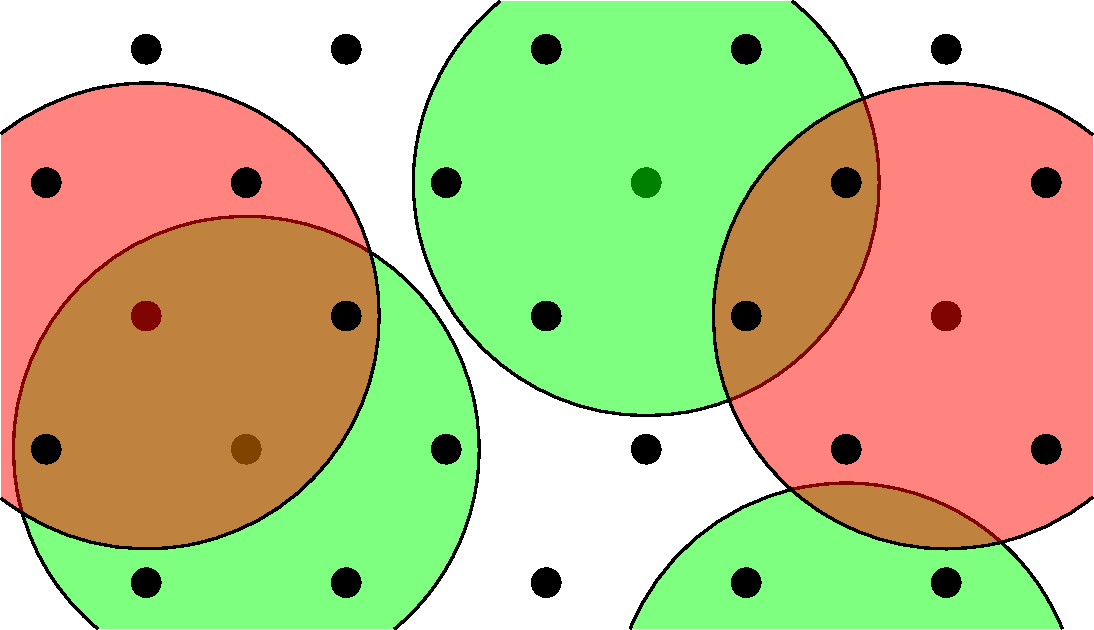
\includegraphics[width=0.5\textwidth]{sterichindrance}
  \caption[Sterische Hinderung]{Sterische Hinderung auf einem Gitter:
    Angelagerte Precursor-Liganden verhindern Reaktionen auf benachbarten Gitterpunkten.
    Überlagerungsfreie Positionen in größerem Abstand akzeptieren weiterhin Precursor-Reaktionen.
  }
  \label{fig:steric}
\end{figure}

\subsection{Simulation von Gasphasenabscheidungen}

\begin{table}
  \centering
  \begin{tabularx}{\textwidth}{XXXX}
    \hline
    Methode & Anwendungsfeld & Größenordnung & Grundlagen \\
    \hline
    Finite Elemente Methode (FEM) & Gasfluss und Verbrauch in Reaktoren & makroskopisch & Navier-Stokes-Gl., Reaktionskinetik \\
    Kinetic Monte Carlo (KMC) & Wachstums\-simulationen & mikroskopisch & Reaktionsraten, Gitternäherungen \\
    Molekular\-dynamik (MD) & Material\-unter\-suchungen & < 1.000.000 Atome & klassische Interaktionspotentiale \\
    Dichte\-funktional\-theorie (DFT) & Reaktionspfade & < 1.000 Atome & Elektronendichten \\
    \hline
  \end{tabularx}
  \caption[Ausgewählte Methoden zur Simulation von Gasphasenabscheidungen]{Ausgewählte Methoden zur Simulation von Gasphasenabscheidungen}
  \label{tab:deposition-simulations}
  \todo[inline]{Referenzen!}
\end{table}

Tabelle \ref{tab:deposition-simulations} stellt ausgewählte Simulationsmethoden für Gasphasenabscheidungen vor, die in der Praxis Anwendung finden.
Besonders auf atomarer Ebene sind viele Prozesse nicht vollends verstanden.
So ist der genaue Reaktionspfad für Precursorpaare oft nicht bekannt, obwohl sie seit Jahrzehnten erfolgreich eingesetzt werden.
Durch Simulationen will man diese Prozesse verstehen helfen und somit genauere Kontrolle über die abgeschiedenen Schichten erlangen.

Dichtefunktionaltheorie und Molekulardynamik stechen hier aufgrund ihrer atomaren Arbeitsweise besonders hervor.
DFT-Untersuchungen beschränken sich hier auf die Reaktionspfade von Molekülen, wo hingegen Molekulardynamik das fertige Material zu simulieren versucht.
In den letzten Jahren sind hingegen auch reaktive Formulierungen für Molekulardynamik aufgekommen\todo{Referenz}, die einen zentralen Bestandteil dieser Arbeit bilden.

\clearpage
\section{Molekulardynamik}

Molekulardynamik (MD) ist im Gegensatz zu quantenmechanischen Methoden eine klassische atomistische Methode, die zwar ungenauere Ergebnisse liefert, jedoch größere Systeme von bis zu einer Million Atome in akzeptabler Zeit rechnen kann.
Damit wird sie seit vielen Jahren erfolgreich in Physik, Chemie sowie in Materialwissenschaften genutzt, um System-, Molekül- und Materialeigenschaften zu bestimmen und Rückschlüsse auf reale Prozesse zu führen.
Somit existiert es eine Vielzahl gut erforschter Systeme, auf die im Rahmen dieser Arbeit aufgebaut wird.

\subsection{Formulierung}

\subsubsection{Allgemeines}

Als klassische Methode arbeitet Molekulardynamik mit Kraftfeldern, Massen.
So besteht ein System aus einer Vielzahl an Teilchen, die als Punktmasse angenähert werden, sowie einer universellen Zeit $t$.
Jedes Teilchen vereint also die Eigenschaften seiner Masse $m$, seines Impulses $\vec p$ und seiner Position $\vec r$.
Zusätzlich wirkt auf jedes Teilchen ein Kraftfeld $F(R)$ mit $R$ als aktuellem Systemzustand.

\subsubsection{Mikrokanonisches Ensemble (NVE)}

Es gilt für jedes Teilchen:

\begin{equation}
  \dot{\vec r} = {\vec p \over m}
\end{equation}

\begin{equation}
  \dot{\vec p} = m \vec a = F(R)
\end{equation}

\todo{Globale Formulierung!}

Zentral ist also das Kraftfeld $F(R)$, welches auf unterschiedliche Arten 

\subsubsection{Kanonisches Ensemble (NVT)}

Gegenüber dem mikrokanonischen Ensemble kommt im Kanonischen Ensemble noch ein Thermostat hinzu.
Dieses gleicht die mittlere Temperatur des Systemes an einen vorgegebenen Wert an.
Dies kann über harte Reskalierung der Atomgeschwindigkeiten (Berendsen-Thermostat), durch zufällige Stöße mit virtuellen Teilchen (Anderson-Thermostat) geschehen, oder durch einen zusätzlichen Reibungsterm, der auch negative Reibungskoeffizienten zulässt (Nosé-\-Hoover-\-Thermostat).

Unter Benutzung des \textbf{Berendsen-Thermostates} werden jeden Zeitschritt die Geschwindigkeiten aller Teilchen so skaliert, dass die Temperatur, die sich aus der kinetischen Energie über die Maxwell-Boltzmann-Verteilung für Gase ergibt, auf dem Zielwert gehalten wird:

\begin{equation}
  \overline{E_{kin}} = {1\over2} m\overline{v^2} = {d\over2}k_BT
\end{equation}

%% \begin{equation}
%% T = {m \overline{v^2} \over k_B d}
%% \end{equation}

Da dabei eine feste Temperatur erzwungen wird, ergibt dieses Thermostat kein kanonisches Ensemble, ist jedoch für große Systeme eine gute Näherung, die effizient berechnet werden kann.

Das \textbf{Anderson-Thermostat} hingegen arbeitet näher an der Idee des kanonischen Ensembles, über die Systemgrenzen hinweg Energie und somit Temperatur durch Teilchenstöße auszutauschen.
Dabei wird für die Zahl der Stöße pro Zeitschritt eine Poissonverteilung angenommen, Masse und Geschwindigkeiten der virtuellen Atome entsprechen der Zieltemperatur.
Zwar hat diese Vorgehensweise den Vorteil, mit einer geringen Anzahl an äußeren Einflüssen die Temperatur konstant zu halten, jedoch eignet es sich nur für die Betrachtung zeitgemittelter Größen.
Durch die Manipulation einzelner, zufälliger Atome können Trajektorien, insbesondere Abscheidungsorte und -konfigurationen stark beeinflusst werden.

Als Alternative eignet sich das \textbf{Nosé-Hoover-Thermostat}.
Dieses fügt dem Gesamtsystem einen zusätzlichen Freiheitsgrad $s$ hinzu, der die Temperatur beeinflusst.
Auf jedes Atom $i$ wirkt somit eine zusätzliche Reibungskraft entlang des Impulses:

\begin{equation}
  \dot{\vec p_i} = \vec{F_i} - s \vec{p_i}
\end{equation}

Der Reibungskoeffizient $s$ ändert sich dabei in Abhängigkeit vom System und kann dabei auch negative Werte annehmen:

\begin{equation}
  \dot s = {\tau \over M} \sum_i{{p_i^2 \over 2m_i} - {Nd \over k_BT}}
\end{equation}

\todo{tau hin oder weg?}

Damit fluktuiert die Temperatur um den Zielwert, wird also nicht fest erzwungen und folgt somit dem kanonischen Ensemble, wobei $\tau$ die Zeitskala angibt, auf der das System ins thermische Gleichgewicht übergeht.
In vielen Softwarepaketen für Molekulardynamiksimulationen dient das Nosé-Hoover-Thermostat als Standardthermostat.

\subsubsection{Großkanonisches Ensemble (NPT)}

Zusätzlich zu einem Thermostat kommt im großkanonischen Ensemble ein Barostat zum Einsatz.
Dieses reguliert über Reskalierung des Simulationsraumes unter periodischen Randbedingungen den mittleren Druck des Systemes.
Dadurch lassen sich periodische Strukturen wie Kristalle frei relaxieren, ohne ihnen eine feste Dichte aufzuzwingen.
Andererseits lassen sich auch Systeme unter großen Drücken untersuchen.

Die Methoden des Barostats gleichen dem des Thermostats, wobei hier nicht die einzelnen Atome, sondern deren relativer Abstand von einander durch Skalierung der Raumposition manipuliert wird.
Als Voreinstellung kommt üblicherweise wieder ein Nosé-Hoover-Barostat zum Einsatz, wobei aufgrund seiner Einfachheit auch Berendsen-Barostate genutzt werden.
Der Druck wird dabei über die Virialgleichung \todo{für ideale Gase?} ermittelt:

\begin{equation}
  PV = Nk_BT + \frac{1}{d} \sum_{i=1}^N{\vec{r}_i \cdot \vec{F}_i}
\end{equation}

\subsubsection{Minimierung durch Konjugierte Gradienten (CG-Minimierung)}

\begin{figure}[!b]
  \centering
  \def\svgwidth{0.8\textwidth}
  \input{img/cg-gradient.pdf_tex}
  \caption[CG-Methode]{Klassische Minimierung durch konjugierte Gradienten:\\
a) Optimale Schrittlänge\\
b) Kleine Schrittlänge $\Rightarrow$ viele unnötige Schritte\\
c) Große Schrittlänge $\Rightarrow$ langsames Konvergenzverhalten
}
  \label{fig:cg-gradient}
\end{figure}

Zur Energieminimierung, welche der Strukturoptimierung dient, wird häufig die \textbf{Methode der konjugierten Gradienten} angewandt.
Man sucht dabei in der Grundvariante ausgehend von einem beliebigen Startpunkt $\vec x_0$ das Minimum der im Suchbereich stetigen Funktion $f(\vec x)$ durch schrittweise Annäherung entlang des Gradienten:

\begin{gather}
  \vec s_i = \Delta\vec x_i = \nabla f(\vec x_{i-1})\\
  \vec x_i = \vec x_{i-1} - \alpha \vec s_i
\end{gather}

Der zusätzliche Parameter $\alpha$ legt dabei die Schrittweite fest.
Mögliche Abbruchkriterien können dabei die Differenz zwischen zwei Schritten ($\left|\vec x_i - \vec x_{i-1}\right| < x_\text{tol}$), die maximale Änderung eines Vektorelementes ($\max_k{\left|x_{i,k} - x_{i-1,k}\right|} < x_\text{tol}$), die Stärke des Gradienten ($\left|\nabla f(\vec x_{i-1})\right| < x_\text{tol}$), eine Anzahl an Zeitschritten ($i > i_\text{tol}$) oder eine Kombination daraus sein.

Dieser grundlegende Algorithmus stößt schnell anseine Grenzen, wenn man allgemeine, nichtlineare Funktionen minimieren möchte.
Dafür führt man mehrere Änderungen ein:
Einerseits ersetzt man den Sprung durch eine Minimierung entlang der Schrittrichtung (Gleichungen \ref{eq:cg-linesearch1} und \ref{eq:cg-linesearch2}).
Andererseits ändert man die Schrittrichtung in Abhängigkeit vorheriger Schritte leicht ab (Gleichungen \ref{eq:pr1} und \ref{eq:pr2}).
Hier wird die Polak-Ribière-Variante vorgestellt1, die standardmäßig in LAMMPS zum Einsatz kommt, jedoch existieren weitere gleichwertige Methoden.

\begin{gather}
  \label{eq:cg-linesearch1}
  \min_\alpha f(x_i+\alpha \vec s_i) \rightarrow \alpha_i \\
  \label{eq:cg-linesearch2}
  \vec x_i = \vec x_{i-1} - \alpha_i \vec s_i\\
  \label{eq:pr1}
  \vec s_i = \Delta \vec x_i + \beta_i \vec s_{i-1}\\
\end{gather}
\begin{equation}
  \label{eq:pr2}
  \beta_i = \max \left(0, \frac{\Delta \vec x_i \cdot \left(\Delta \vec x_i - \Delta \vec x_{i-1}\right)}{\Delta \vec x_{i-1} \cdot \Delta \vec x_{i-1}}\right) \text{ (Polak-Ribière)}
\end{equation}

Diese Anpassungen verbessern einerseits das erwartete Konvergenzverhalten, andererseits stabilisieren sie den Optimierungsalgorithmus gegenüber Nichtlinearitäten und Unstetigkeiten\todo{Referenz? Lüge?}.

\subsubsection{Weitere Minimierungsmethoden}

Es stehen noch weitere Minimierungsalgorithmen zur Verfügung, wie beispielsweise die Klasse der Newton-Verfahren.
Obwohl diese auf dem Papier schneller konvergieren, sind für jeden Iterationsschritt durch die Berechnung der Hesse-Matrix mehr Rechenoperationen notwendig, so dass reale Berechnungszeit und Speicherverbrauch gegenüber CG-Methoden oft im Nachteil sind.
\todo{Referenz für Interessierte}

\subsection{Kraftfelder}

Basis aller im vorherigen Abschnitt vorgestellten Methoden sind stets Kraftfelder, die die gewünschte Struktur darstellen können.
Hierfür gibt es eine Vielzahl an verschiedenen Formulierungen, für die es jeweils verschiedene Parametrisierungen gibt, um bestimmte Systeme und Umgebungen zu betrachten.

\subsubsection{Paar-Potentiale}

\missingfigure{Lennard-Jones, Buckingham, Hartkugel}

Das klassische MD-Potential ist das Paarpotential, welches eine Interaktion zwischen zwei benachbarten Atomen modelliert.
Stellvertretend sind beispielsweise das Lennard-Jones-Potential zur Darstellung von allgemeinen Fluiden (Gleichung \ref{eq:lennardjones}) oder das damit verwandte Bucking\-ham-Potential.

\begin{equation}
  \label{eq:lennardjones}
  V_{LJ}(r_{ij}) = 4 \epsilon \left[\left(\frac{\sigma}{r_{ij}}\right)^{12} - \left(\frac{\sigma}{r_{ij}}\right)^{6}\right]
\end{equation}
\begin{equation}
  \label{eq:pairforce}
  \vec F_{ij}(\vec r_{ij}) = \vec\nabla V(r_{ij})
\end{equation}
\begin{equation}
  \label{eq:pairenergy}
  E = \sum_i\sum_{j \neq i}{V_{LJ}\left(r_{ij}\right)}
\end{equation}

Andere Potentiale enthalten weitere Parameter oder tabellierte Werte, mit denen spezielle Probleme genauer betrachtet werden können.
Das allgemeine Problem der Klasse der Paarpotentiale ist ihre Schlichtheit.
So lassen sie sich schwer an realistische Strukturen fitten und können oftmals nur ein Material in einem Szenario darstellen, wobei sie allerdings schnell sind.

\subsubsection{N-Teilchen-Potentiale}

N-Teilchen-Potentiale  erweitern Paarpotentiale um weitere Terme, die von einer festen Anzahl an Teilchen abhängen, beispielsweise Winkel- und Torsionsabhängigkeiten.

\begin{equation}
  \label{eq:nbody-energy}
  E = \sum_i\sum_{j \neq i}{V_2\left(r_{ij}\right)} + \sum_i\sum_{j \neq i}\sum_{i \neq k \neq j}{V_3\left(r_{ij}, r_{ik}, \theta_{ijk}\right)}
\end{equation}
\todo{letzte Summe: Indizes aufspalten}

Obwohl sich mit N-Teilchen-Potentialen komplexere Systeme betrachten lassen, zeigen sie die gleichen Schwachstellen wie Paarpotentiale.
Zwar gibt es erfolgreiche \todo{kommerzielle} Anpassungen für Biomoleküle (\todo{CHARMM} \todo{GROMACS} \todo{AMBER}), die allerdings nicht auf andere Stoffsysteme übertragbar sind.

\subsubsection{Embedded Atom Model}

Das Embedded Atom Model (EAM) für jedes Atom $i$ besteht aus einem Paarpotential $V_{\alpha\beta}(r_{ij})$ sowie einer Einbettungsfunktion $F_\alpha$, die die Energie jedes Atomes in Abhängigkeit der angenäherten Elektronendichte $\rho_\beta(r_{ij})$ in der Umgebung modelliert (Gleichung \ref{eq:eam-energy}).\todo{Referenz}
So lassen sich insbesondere metallische Materialien und Oberflächen simulieren.
$\alpha$ und $\beta$ stellen dabei verschiedene Atomsorten dar, allerdings lassen sich auch mit dieser umfangreicheren Formulierung hauptsächlich reine Metalle simulieren.
Für diese findet man allerdings passende Parametrisierungen\todo{Referenz auf Datenbank und passende Paper}, die im Gegensatz zu den meisten Potentialen sowohl thermisches Verhalten als auch Strukturen recht gut modellieren \todo{Referenz auf separates Ergebniskapitel}.

\begin{equation}
  \label{eq:eam-energy}
  E = \sum_i\left[F_\alpha\left(\sum_{j\neq i}{\rho_\beta\left(r_{ij}\right)}\right) + \frac{1}{2}\sum_{j\neq i}{V_{\alpha\beta}\left(r_{ij}\right)}\right]
\end{equation}

\subsubsection{Modified Embedded Atom Model}

Um die Einschränkung des reinen EAM-Potentials zu umgehen, wurde das Modified Embedded Atom Model (MEAM) erforscht (Gleichung \ref{eq:meam-energy}). \todo{Referenz auf Baskes}
Mit diesem lassen sich auch Metalloxide, Legierungen und andere Mischsysteme untersuchen\todo{Referenz}.

\todo{Wie funktioniert es?}

\begin{equation}
  \label{eq:meam-energy}
  E = \sum_i\left[F_\alpha\left(\bar{\rho_i}\right) + \frac{1}{2}\sum_{j\neq i}{V_{ij}\left(r_{ij}\right)}\right]
\end{equation}

Wie beim EAM-Potential sind die eigentlichen Berechnungen in den einzelnen Funktionen versteckt, die auf umfassende Weise die Elektronendichten zu modellieren versuchen.
Dafür ist vorher eine umfangreichere Parametrisierung notwendig, die an eine Vielzahl von Strukturen gefittet werden muss.

\subsubsection{Reactive Force Fields}

\todo{Referenz}
Reactive Force Fields (ReaxFF) wurden mit der Idee erdacht, bisher unmögliche Simulationen in Molekulardynamik mit größeren Systemen darstellen zu können.
Dafür fließt eine Vielzahl an Einflüssen in die Potentialgestaltung ein, beispielsweise Van-der-Waals-Kräfte und elektrostatische Kräfte, allerdings ist der zentrale Gedanke die Modellierung von Über- und Unterkoordination eines Atomes in seiner Nachbarschaft unter Ladungsaustausch.
Somit lassen sich Bindungen während der Simulation dynamisch formen und lösen und dadurch ganze Reaktionen zwischen verschiedenen Molekülen simulieren.

\begin{align}
  \label{eq:reax-formulation}
  E_\text{system} &= E_\text{bond} + E_\text{lp} + E_\text{over} + E_\text{under} + E_\text{val} + E_\text{pen} + E_\text{coa} + E_\text{C2} \\
\nonumber  & + E_\text{tors} + E_\text{conj} + E_\text{H-bond} + E_\text{vdWaals} + E_\text{Coulomb}
\end{align}

Die meisten Terme der Gesamtenergie werden über die Bindungsordnung berechnet, die über Beiträge für $\sigma$-, $\pi$- und Doppel-$\pi$-Bindungen aus dem Bindungsabstand errechnet wird.
Einige werden durch Taper-Korrektur\todo{ref} in der Nähe des Cutoff-Abstandes auf 0 gesenkt, um Diskontinuitäten zu vermeiden und einen fließenden Übergang zwischen Bindungszuständen zu ermöglichen.

\todo{Referenz auf Equations\_Reax.pdf}

\begin{table}
  \begin{tabularx}{\textwidth}{llX}
    \hline
    Term & Beitrag & Kommentar \\
    \hline
    $E_\text{bond}$ & Bindungsenergien & Berechnung über Bindungsordnung\\
    $E_\text{lp}$ & freie Elektronenpaare & über Bindungsordnungssumme am Atomzentrum\\
    $E_\text{over}$ & Überkoordinationen & unter Ausschluss freier Elektronenpaare\\
    $E_\text{under}$ & Unterkoordinationen & nur bei unterkoordinierten $\pi$-Bindungen\\
    $E_\text{val}$ & Bindungswinkel & Optimum abhängig von Elektronenkonfiguration\\
    $E_\text{pen}$ & Strafenergien & Fehlerkorrektur bei Winkeln mit Doppelbindung\\
    $E_\text{coa}$ & Drei-Teilchen-Konjugationen & Stabilisierung von NO$_2$-Gruppen\\
    $E_\text{C2}$ & Dreifachbindungskorrektur & Stabilisierung der Dreifachbindung von C$_2$\\
    $E_\text{tors}$ & Torsionsbarrieren & \\
    $E_\text{conj}$ & Vier-Teilchen-Konjugationen & Konjugation bei Kohlenwasserstoffen\\
    $E_\text{H-bond}$ & Wasserstoffbrücken & \\
    $E_\text{vdWaals}$ & Van-der-Waals-Kräfte & \\
    $E_\text{Coulomb}$ & Coulomb-Kräfte & \\
    \hline
  \end{tabularx}
  \caption[ReaxFF Energiebeiträge]{ReaxFF Energiebeiträge aus Gleichung \ref{eq:reax-formulation}}
  \label{tab:reax-energies}
\end{table}

Wie aus Gleichung \ref{eq:reax-formulation} und Tabelle \ref{tab:reax-energies} hervor geht, wurden das ReaxFF-Potential ursprünglich für Reaktionen von organischen Molekülen entwickelt, ist aber vielseitig genug, eine Vielzahl anderer Materialien simulieren zu können.
Die unterstützten Stoffgruppen hängen dabei stark von den Strukturen ab, an die die Parametrisierung gefittet wurde.
Auch, wenn alle notwendigen Atomsorten unterstützt werden, kommt es häufig vor, dass der zu untersuchende Stoff bei der Parametersuche nicht beachtet wurde und somit nicht darstellbar ist.

In den letzten fünf Jahren haben Reactive Force Fields jedoch langsam an Aufmerksamkeit gewonnen, so dass die Zahl spezialisierter Parametrisierungen wächst.
Es gibt auch Bestrebungen, sich ergänzende ReaxFF-Parametrisierungen zu kombinieren und somit mit einer Parametrisierung jedes gewünschte System betrachten zu können.
Besonders in kommerzieller MD-Software\todo{Referenz auf GULP} versucht man so, dem Nutzer unnötige Arbeit abzunehmen.
Es muss sich jedoch noch zeigen, ob dieser Ansatz zufrieden stellende Ergebnisse liefern kann.

\subsubsection{Allgemeine Probleme}

\textbf{Parametrisierung}:
Da Molekulardynamik keine ab-initio-Methode ist, sondern jedes Potential erst an experimentelle oder numerische Daten angepasst (gefittet)\todo{was nun?} werden muss, sollte die Herkunft jeder Parametrisierung bei seiner Nutzung bedacht werden.
\todo{kulkarni: Kritische Betrachtung seiner Trainingsstrukturen}
\\\\
\textbf{Übertragbarkeit}:
Je nach Potentialart lassen sich viele Parametrisierungen nicht vermischen oder auf andere Probleme übertragen.
\\\\
\textbf{Analysemethoden}:
Im Normalfall sind Potentiale entweder für strukturelle oder thermische Größen optimiert.
Mit einem rein strukturellen Potential lassen sich also keine thermischen Größen und Phasenübergänge verlässlich ermitteln.
\\\\
\textbf{Reaktionen}:
Mit der Ausnahme des ReaxFF-Potentiales lassen sich per Molekulardynamik keine Reaktionen betrachten.
\\\\
\textbf{Annäherungen}:
\todo{Was hast du hier gedacht, Erik?}

\subsection{Auswertung}

\subsubsection{Relaxierungen}

\subsubsection{Struktur}

Zur Auswertung einer Struktur bietet sich zuerst eine visuelle Beurteilung an, die mit entsprechenden Programmen vorgenommen werden kann.
Damit können grobe Defekte ausgeschlossen werden.

\subsubsection{Dichte}

Die Dichte lässt sich bei periodischen Strukturen nach über Volumen und 

\subsubsection{Radiale Verteilungsfunktionen}

\subsubsection{Oberfläche}

Die Oberfläche einer Struktur gibt Hinweise auf angelagerte Molekülgruppen, Rauheit, Porösität und Bildung reinatomiger Cluster.
Bei großen, glatten Strukturen reicht oft ein Schnitt entlang einer Hauptachse, um Bulk und Oberfläche zu trennen.
In den verbliebenen Fällen lässt sich zu diesem Zweck eine Alpha-Form per Delaunay-Triangulation bestimmen. \todo{Referenz auf Delaunay-Section}
Die eigentlichen Untersuchungen beschränken sich dann auf eine Zählung der Bindungen und Atomsorten, Radiale Verteilungsfunktionen, Oberflächenmessung oder Höhenabweichung vom Mittelwert.

\subsubsection{Reaktionen}



\subsection{Software}

Für molekulardynamische Simulationen gibt es sowohl kommerzielle als auch freie Softwarepakete, die einige Parametersätze mitbringen.
Tabelle \ref{tab:mdsoftware} stellt eine Auswahl daraus dar.

\begin{table}
  \begin{tabularx}{\textwidth}{llX}
    \hline
    Paket & Rechteinhaber & Kommentare \\
    \hline
    LAMMPS & SANDIA & quelloffen, CLI-bedienbar, Bibliothek, eigene Potentiale möglich \\
    Materials Studio GULP & Accelrys & Tief in graphischer Oberfläche verankert \\
    AMBER & University of California & verschiedene Biomoleküle \\
    CHARMM & Accelrys & Proteine \\
    GROMACS & Uppsala University & Biomoleküle, quelloffen \\
    \hline
  \end{tabularx}
  \todo[inline]{References!}
  \todo[inline]{bessere Beschreibung!}
  \caption[MD-Software]{MD-Software}
  \label{tab:mdsoftware}
\end{table}


\clearpage
\section{Kinetic Monte Carlo-Methoden}

Kinetic Monte Carlo-Methoden bezeichnen zufallsbestimmte numerische Prozesse, bei denen das System eine Reihe von diskreten Zuständen durchläuft, die auf Basis einer Übergangswahrscheinlichkeit aus dem vorhergehenden Zustand zufällig gewählt werden.
Ursprünglich für die Simulation von  Diffusionsprozessen entwickelt, finden sie inzwischen in vielen Gebieten der Natur- und Ingenieurswissenschaften Anwendung, insbesondere auch für Nichtgleichgewichtssysteme wie  Oberflächenreaktionen und Schichtabscheidungen.

Die mathematische Formulierung folgt Markov-Ketten, die eine Abfolge von Zuständen $X_t$ aus einem abzählbar großen Zustandsraum $S$ darstellen. ASD

$$
X_t = S \forall t \geq 0
$$
$$
X_{t+\Delta t} = E(X_t, t)
$$
$$
\Delta t = - \frac{\ln(u)}{r_i}
$$


\clearpage
\section{Datenstrukturen}
\label{datastructures}

Zur Beschleunigung von atomistischen Simulationen mit Parsivald finden effiziente Algorithmen zur Suche und Manipulation von Atomen auf Basis verschiedener Datenstrukturen Anwendung, welche im Folgenden zwecks der Beschreibung von Atompositionen in teilperiodischen Simulationsräumen für Off-Lattice-KMC-Simulationen untersucht werden sollen.
Gegenüber optimalen Algorithmen für allgemeine Probleme, wie sie in verfügbarer Software genutzt werden, ermöglicht die genaue Modell- und Systemkenntnis die Abwägung der Häufigkeit von Operationen gegen deren Laufzeiten,
wodurch die Wahl der optimalen Datenstruktur zur Maximierung von Größe, Genauigkeit und Geschwindigkeit von Off-Lattice-KMC-Simulationen von Gasphasenabscheidungen ermöglicht wird.

\subsection{Numerische Voraussetzungen an Gasphasenabscheidungen}

Für eine effiziente KMC-Simulation werden für zu untersuchende Gasphasenabscheidungen folgende Voraussetzungen getroffen:
Zuerst sollten die KMC-Ereignisse \textbf{lokal}, also auf eine geringe Reichweite begrenzt sein.
Das bedeutet auch, dass die Atome über \textbf{niedrige Diffusionskoeffizienten} verfügen, was sich aus der Notwendigkeit ergibt, im statischen Gleichgewicht befindliche Bereiche des Simulationsraumes von atomistischen Simulationen auszuschließen.
Weiterhin werden \textbf{scharfe Phasengrenzen} vorausgesetzt, also zweidimensionale Grenzflächen, die sich durch eine vergleichsweise geringe Menge von Atomen darstellen lassen.
Zuletzt finden die Simulationen aus praktischen Gründen in \textbf{teilperiodischen Räumen} statt, also Räumen, die in der xy-Ebene periodisch, aber in z-Richtung beliebig ausgedehnt sein können.

%% Daraus ergeben sich jeweils Vor- und Nachteile für verschiedene Datenstrukturen, so dass etwa für die Vereinigung zweier disjunkter Triangulation (Stitching) in periodischen Räumen zusätzlicher Aufwand gegenüber nichtperiodischen Räumen betrieben werden muss.
%% Die größten Vorteile ergeben sich aus der Lokalität von Ereignissen, da so für die meisten Datenstrukturen nur kleine Teilstrukturen überprüft und aktualisiert werden müssen.

\subsection{Vergleich der Laufzeiten mit verschiedenen Datenstrukturen}

Als Datenstrukturen stehen \textbf{Atomlisten}, \textbf{Nachbarschaftslisten} (NB-Listen), lineares \textbf{Binning}, Binning in \textbf{Octrees}, \textbf{k-d-Bäume} und \textbf{Delaunay-Triangulationen} zur Auswahl.
%, von denen eine Auswahl in Abbildung~\ref{fig:datastructures} dargestellt ist.
In Anhang~\ref{appendix_dataoverview} werden diese knapp vorgestellt, wobei auf die drei zuletzt genannten in den folgenden Abschnitten näher eingegangen wird.

Atomistische KMC-Simulationen beschränken sich auf die Manipulations-Operationen zur \textbf{Einfügung}, \textbf{Modifikation} und \textbf{Entfernung} von Atomen, \textbf{Konstruktion} der Datenstruktur sowie auf die Suchoperationen der \textbf{Nachbarschaftssuche}, \textbf{Bereichssuche} und \textbf{Oberflächensuche}, die jeweils in Anhang~\ref{dataops} kurz beschrieben werden.
Die Effizienz dieser Operationen geht dabei aus deren asymptotischer Laufzeit hervor, welche üblicherweise in asymptotischer Notation (\BigO{}) angegeben wird.

Bei KMC-Simulationen überwiegen die drei Suchoperationen, da sie für jedes Ereignis beim Aufbau der KMC-Ereignislisten durchgeführt werden müssen, wo hingegen die Manipulationen nur für das tatsächlich durchgeführte Ereignis ausgeführt werden müssen.
Somit liegt das Auswahlkriterium der Datenstruktur bei der Effizienz ihrer Suchoperationen, mit Ausnahme der Nachbarschaftslisten und k-d-Bäume, deren Manipulationsoperationen für große Simulationsräume \todo{phrasing}zu langsam sind.
Die Ergebnisse der Laufzeit-Analysen der sieben Operationen auf den vorgestellten Datenstrukturen werden in Tabelle~\ref{tab:dataruntimes} zusammen gefasst, wofür Tabelle~\ref{tab:datasymbols} die verwendeten Symbole erklärt.

\begin{table}[!ht]
  \centering

  \caption{Abschätzung der Komplexität für verschiedene Datenstrukturen und Operationen}
  \label{tab:dataruntimes}
  \begin{tabularx}{\textwidth}{|X|*8c|}
    \hline
    \textbf{Datenstr.} & Konstr.         & Einfüg.         & Modif.          & Entf.           & Ortss.                     & NB-Su.              & Oberfl.        & RAM                         \\
    \hline
    Atomlisten         & \cG{$n$}        & \cG{$1$}        & \cG{$1$}        & \cG{$1$}        & \cR{$n$}                   & \cR{$n$}            & \cR{$n$}       & \cG{$n$}                    \\
    NB-Listen          & \cY{$n\log{n}$} & \cR{$n$}        & \cR{$n$}        & \cR{$n$}        & \cR{$n$}                   & \cG{$1$}            & \cR{$n$}       & \cR{$\frac{r_c^3}{s^3}n^2$} \\
    Binning            & \cG{$n$}        & \cG{$1$}        & \cG{$1$}        & \cG{$1$}        & \cG{$r_s^3$}               & \cG{$r_s^3$}        & \cR{$c$}       & \cY{$n+c$}                  \\
    Octree             & \cY{$n\log{c}$} & \cY{$\log{c}$}  & \cY{$\log{c}$}  & \cG{$1$}        & \cY{$r_s^3\log{c}$}        & \cY{$r_s^3\log{c}$} & \cY{$\log{c}$} & \cY{$n+c^\frac{2}{3}$}      \\
    k-d-Baum           & \cY{$n\log{n}$} & \cY{$\log{n}$}  & \cY{$\log{n}$}  & \cY{$\log{n}$}  & \cY{$r_s^3\log{n}$}        & \cY{$r_s^3\log{n}$} & \cY{$\log{n}$} & \cG{$n$}                    \\
    Delaunay           & \cY{$n\log{n}$} & \cY{$k\log{k}$} & \cY{$k\log{k}$} & \cY{$k\log{k}$} & \cG{$r_s^3+n^\frac{1}{3}$} & \cG{$r_s^3$}        & \cG{$1$}       & \cY{$nk$}                   \\
    \hline
    %Atomfeld          & \cG{$n$}        & \cG{$1$}        & \cG{$1$}        & \cG{$1$}        & \cR{$n$}                   & \cR{$n$}            & \cR{$n$}       & \cG{$n$}                    \\
  \end{tabularx}
  \vspace{1em}
  \hspace{0.15\textwidth}
  \begin{tabularx}{0.6\textwidth}{|C|C|C|}
    \hline
    \cG{optimal} & \cY{vertretbar} & \cR{ineffizient} \\
    \hline
  \end{tabularx}

  \vspace{1em}

  \oddrowcolors
  \caption{Symbole für Laufzeit- und Speicherabschätzungen}
  \label{tab:datasymbols}
  \begin{tabularx}{\textwidth}{|cX|cX|}
    \hline
    \textbf{Symbol} & \textbf{Bedeutung}                 & \textbf{Symbol} & \textbf{Bedeutung} \\
    \hline
    \BigO{}         & Worst-Case-Komplexität             & $n$             & Zahl der Atome     \\
    $k$             & Zahl von Nächstnachbarn            & $b$             & Zahl der Bins      \\
    $k_r$           & Zahl von Nachbarn mit $d \leq r_c$ & $r_c$           & Cutoff-Radius      \\
    $r_s$           & Suchradius                         & $s$             & lineare Raumgröße  \\
    \hline
  \end{tabularx}

\end{table}

\clearpage
\subsection{Effiziente Datenstrukturen}

Beim Vergleich der Datenstrukturen in Tabelle~\ref{tab:dataruntimes} stellen sich Octrees, k-d-Bäume und Delaunay-Triangulationen als Favoriten für Off-Lattice KMC-Simulationen heraus, die in den folgenden Abschnitten kurz eingehender vorgestellt und diskutiert werden sollen.
Der Speicherverbrauch der untersuchten Datenstrukturen ist praktisch linear und bildet deshalb kein Auswahlkriterium.
Wie Untersuchungen an Simulationsräumen verschiedener Größe zeigen, wird erst für \num{1.9e9} Atome die Grenze des Hauptspeichers erreicht (Abschnitt~\ref{goldscalability}).

\subsubsection{Octrees}
\label{dataoctree}

Octrees sind eine Optimierung raumfüllender orthogonaler Partitionierungen, wie sie üblicherweise für Binning-Methoden genutzt werden, bei der statt linearer Adressierung auf einen mehrdimensionalen Binärbaum zurück gegriffen wird, woher auch der Name stammt (1D: Binary Tree, 2D: Quadtree, 3D: Octree, etc.).
Der Simulationsraum wird rekursiv in jeweils 8 disjunkte geometrisch ähnliche Unterzellen halber Breite aufgeteilt, wodurch die eigentlichen Bins in der festen Tiefe $\frac{\log{c}}{d\log{2}}$ liegen.

Damit steigt die Adressierungszeit für einzelne Zellen auf \BigO{\log{c}}, doch werden nur die Bins allokiert, die tatsächlich gefüllt sind (Abbildung~\ref{fig:octree}), wodurch leere Superzellen bei Suchoperationen automatisch übergangen werden.
Als Resultat sind für Oberflächensysteme der Speicherbedarf und die Laufzeit von Suchoperationen eines dreidimensionalen Simulationsraumes auf die eines zweidimensionalen Systemes reduziert.
Theoretisch sind mit Access Caching, Bitweiser Adressierung, Surface Flagging oder Height Mapping noch weitere Anpassungen möglich, allerdings verbessert sich dabei nur der Laufzeitfaktor, nicht die asymptotische Laufzeit, weshalb sie nur am Rand genannt sein sollen.

%% \begin{algorithm}
%%   \begin{algorithmic}
%% %    \Input $atoms$ - Liste der Atome
%% %    \Input $size[3]$ - Größe des Simulationsraumes
%% %    \Input $depth$ - Tiefe des Octrees (Legt die Zellgröße fest)
%% %    \Assumption Alle Atome befinden sich im Simulationsraum
%% %    \Result Stammzelle eines Octrees, der alle Atome enthält
%%     \State
%%     \Function{construct-octree}{$atoms, spacesize, depth$}
%%     \State $cellsize[0] \gets spacesize[0]\cdot2^{-depth}$
%%     \State $cellsize[1] \gets spacesize[1]\cdot2^{-depth}$
%%     \State $cellsize[2] \gets spacesize[2]\cdot2^{-depth}$
%%     \State $root \gets$ new Octree($depth$)
%%     \ForAll{$atom$ in $atoms$}
%%     \State $cellindex[0] \gets \lfloor atom.pos[0] / cellsize[0] \rfloor$
%%     \State $cellindex[1] \gets \lfloor atom.pos[1] / cellsize[1] \rfloor$
%%     \State $cellindex[2] \gets \lfloor atom.pos[2] / cellsize[2] \rfloor$
%%     \State $cell \gets$ \Call{getcell-octree}{$root, cellindex$, true}
%%     \State \Call{add-atom}{cell, atom}
%%     \EndFor
%%     \State \Return $root$
%%     \EndFunction
%%   \end{algorithmic}
%%   \caption[Octree-Konstruktion]{Octree-Konstruktion: Es handelt sich um einen typischen Binning-Algorithmus, dessen Octree-Eigenschaften in der Funktion \Call{getcell-octree}{} liegen.}
%%   \label{alco:octree-construction}
%% \end{algorithm}

\begin{figure}
  \centering
  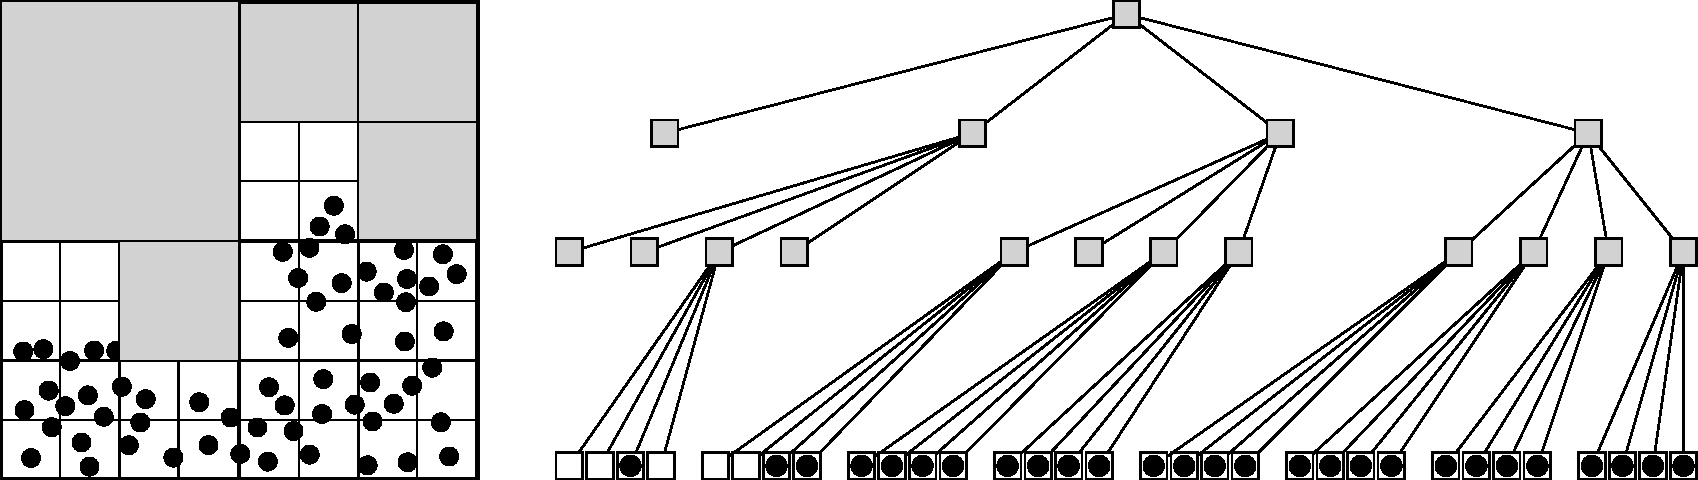
\includegraphics[width=\textwidth]{octree}
  \caption[Veranschaulichung der Funktionsweise eines Octrees]{
    Quadtree zur Veranschaulichung der Funktionsweise eines Octrees:\\
    Räumliche Unterteilung eines Raumes mit zugehörigem Baum von Zellen.
  }
  \label{fig:octree}
\end{figure}

%% \begin{algorithm}
%%   \begin{algorithmic}
%%     %    \Input $root$ - Stammzelle des Octrees
%%     %    \Input $i[3]$ - globale Adresse der Zielzelle
%%     %    \Input $allocate$ - Ob die Zelle neu erstellt werden soll
%%     \Result null falls leer, sonst Zielzelle
%%     \State
%%     \Function{getcell-octree}{$cell, id, allocate$}
%%     \State $d \gets $\Call{depth}{root}
%%     \Comment{Relative Tiefe, an der sich die Zielzellen befinden}
%%     \If{$d = 0$}
%%     \State\Return cell
%%     \EndIf
%%     \If{not $cell.children$}
%%     \If{allocate}
%%     \State $cell.children \gets $new cell[8]
%%     \Else
%%     \State \Return null
%%     \EndIf
%%     \EndIf
%%     \State $childid \gets $\Call{bitand}{id[0], $2^{d-1}$}
%%     + $2\cdot$\Call{bitand}{id[1], $2^{d-1}$}
%%     + $4\cdot$\Call{bitand}{id[2], $2^{d-1}$}
%%     %    \State \Comment{Indiziert die Subzelle aus der globalen Position}
%%     \State \Return\Call{getcell-octree}{$cell.children[childid], i, allocate$}
%%     \EndFunction
%%   \end{algorithmic}
%%   \caption[Zell-Adressierung in Octrees]{Rekursive Zell-Adressierung und -Allokierung im Octree: Bei jedem Schritt wird das Problem in 8 Unterzellen geteilt, woraus eine Laufzeit von \BigO{d}$=$\BigO{\log{c}} resultiert}
%%   \label{algo:octreeaddressing}
%% \end{algorithm}

\subsection{k-d-Bäume}
\label{datakdtree}

Für Nachbarschafts- und Bereichssuchen wird wegen ihrer hervorragenden Sucheffizienz oft auf k-d-Bäume zurückgegriffen, die einen kartesischen Raum in orthogonale Zellen mit jeweils einem Atom unterteilen, wodurch sich ein balancierter Binärbaum ergibt, an dessen Knoten die Atome liegen.
Durch implizite Betrachtung von Abstandsrelationen bei der Konstruktion (Abbildung~\ref{fig:kdtree}) lassen sich Abstands- oder Bereichssuchen in \BigO{\log{n}} durchführen, während Nachbarschaftssuchen von $N$ Atomen in Kombination mit einem Heap in \BigO{\log{n}\log{N}} möglich sind.

Nachteile ergeben sich bei Modifikationen von Atomen, die durch Baumrotation in \BigO{\log{n}} aufgelöst werden müssen und im schlimmsten Fall\footnote{Der schlimmste Fall (engl. \textit{worst case}) besteht in einer Menge von Eingabedaten, die zur größtmöglichen Laufzeit führen} den gesamten Baum neu strukturieren.
Durch die einseitige, dichte und gleichverteilte Hinzufügung von Atomen während einer Oberflächenabscheidung ist dieser Fall allerdings gegeben, da sich der Median der Atompositionen in z-Richtung stetig verschiebt.
Deshalb bieten sich k-d-Bäume zwar für allgemeine Suchoperationen in statischen Off-Lattice-Strukturen an, sind aber nicht für effiziente KMC-Simulationen geeignet.

\begin{figure}
  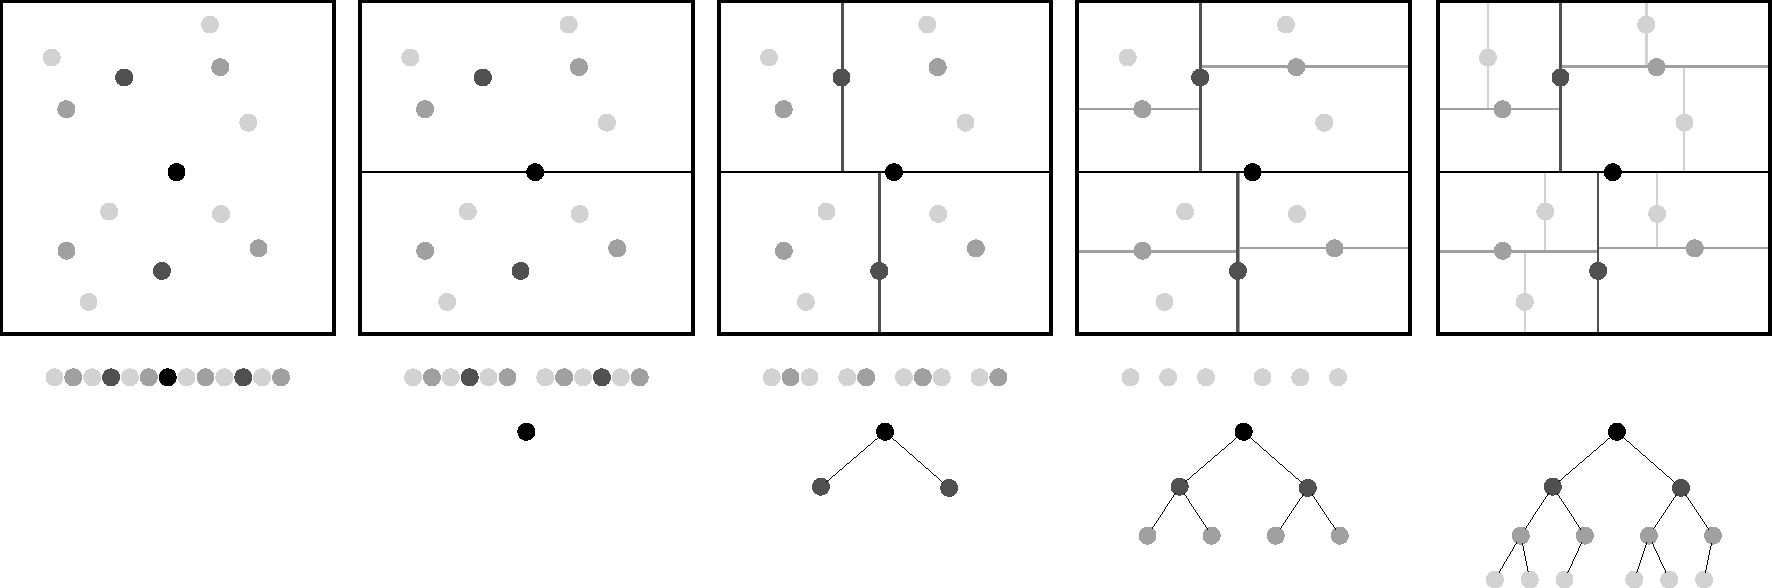
\includegraphics[width=\textwidth]{kdtree-tree}
  \caption[Konstruktion eines k-d-Baumes]{
    Konstruktion eines k-d-Baumes:
    Der Median der sortierten Punkte wird zur Wurzel des Baumes; die beiden Teilmengen rekursiv zu k-d-Bäumen
  }
  \label{fig:kdtree}
\end{figure}

%% \begin{algorithm}
%%   \begin{algorithmic}
%%     \Input $points$ - Liste von Punkten
%%     \Input $k$ - Dimensionalität des Simulationsraumes
%%     \Result Root-Element eines vollständigen k-d-Baumes aus diesen Punkten
%%     \State
%%     \Function{construct-kdtree}{$points, dim\gets0$}
%%     \State $n\gets$\Call{length}{points}
%%     \If{$n=0$}
%%     \State \Return null
%%     \Else
%%     \State \Call{sort}{$points, dim$} \Comment{Sortiert $points$ nach pos[$dim$]}
%%     \State $root\gets{}points\left[\lfloor\frac{n}{2}\rfloor\right]$
%%     \State $dim\gets(dim+1)\mod{k}$
%%     \State $root.left \gets$ \Call{construct-kdtree}{$points\left[0:\lfloor\frac{n}{2}\rfloor-1\right], dim$}
%%     \State $root.right \gets$ \Call{construct-kdtree}{$points\left[\lfloor\frac{n}{2}\rfloor+1:n-1\right], dim$}
%%     \State \Return $root$
%%     \EndIf
%%     \EndFunction
%%   \end{algorithmic}
%%   \caption[Konstruktion eines k-d-Baumes]{Rekursive Konstruktion eines k-d-Baumes (naive Implementierung)}
%%   \label{algo:kdtree-construction}
%% \end{algorithm}

\subsection{Delaunay-Triangulation}
\label{datadelaunay}

\begin{figure}
  \centering
  \def\svgwidth{\textwidth}
  \input{img/delaunay.pdf_tex}
  \caption[Beispiel des Delaunay-Kriteriums]{
    In der Delaunay-Triangulation (c) einer Punktwolke (a) dürfen sich keine weiteren Punkte im Umkreis jedes Simplexes (b) befinden
  }
  \label{fig:delaunay}
\end{figure}

Eine dritte Partitionsmethode findet sich in der Delaunay-Triangulation\todo{Ref?}, welche jedoch asymmetrisch und nicht-orthogonal arbeitet, indem die konvexe Hülle der Punktwolke raumfüllend in disjunkte k-dimensionale Simplexe\footnote{Ein $k$-Simplex ist ein Objekt in $k$ Dimensionen mit $k+1$ Eckpunkten, die untereinander mit geraden Kanten verbunden sind. Somit ist ein 1-Simplex eine Linie, ein 2-Simplex ein Dreieck, ein 3-Simplex ein Tetraeder, etc.}
entsprechend des Delaunay-Kriteriums, nach dem sich im Umkreis eines Simplexes keine anderen Punkte der Punktwolke befinden dürfen, zerlegt wird.
\todo{Anmerkung von Jörg: puuuhhh Du wirst hier ne ganze Menge Dine in den Raum, die eigentlich nach Erklärungen verlangen ...}
Damit ergibt sich ein Graph, der ein Supergraph des Nächstnachbargraphen\footnote{Der Nächstnachbargraph verbindet alle Punkte des Graphen mit ihrem nächsten Nachbarn}, der Alpha-Form (Abschnitt~\ref{dataalphaform}) sowie der konvexen Hülle\footnote{Die konvexe Hülle ist ein Körper aus Dreiecken, der alle Punkte der Punktwolke einschließt. Sie ergibt sich als Vereinigung einer vollständigen Triangulation. Siehe Abbildung~\ref{fig:delaunay-alpha-b}} der Punktwolke ist und in \BigO{n\log{n}} effizient konstruiert werden kann.
Die Konstruktion lässt sich im Gegensatz zu den anderen Datenstrukturen für große Simulationsräume mit entsprechenden Divide-and-Conquer-Algorithmen parallelisieren, oder vor einer etwaigen periodischen Erweiterung einer Einheitszelle zum Simulationsraum durchführen.
Eine Liste von Eigenschaften der Simplexe sowie einer Übersicht über die verschiedenen Konstruktionsmethoden ist in Anhang~\ref{appendix_delaunay} zu finden.

Delaunay-Triangulationen werden noch nicht direkt im KMC-Algorithmus für Off-Lattice-Systeme genutzt, doch sind sie aufgrund ihrer Beziehung zu Alpha-Formen für die Analyse von Oberflächen unentbehrlich (Abschnitt~\ref{mdmethods}).

\subsection{Alpha-Form}
\label{dataalphaform}

Delaunay-Triangulationen werden für Betrachtungen von Oberflächen interessant, da sie die konkave Oberfläche von Punktwolken über die Alpha-Form bestimmen können.
Sie werden durch Vereinigung genau der Simplexe konstruiert, deren Umkreisradius $r_d$ unterhalb einer frei wählbaren Grenze $\alpha$ liegt, oder durch komplementäre Algorithmen, wie sie in Abbildung~\ref{fig:delaunay-alpha} veranschaulicht sind.
Als Resultat ergibt sich eine Menge von Punkten und Dreiecken, welche die scheinbare Oberfläche der Punktwolke bilden, die für weitere Untersuchungen wie die Bestimmung von Oberflächenrauheiten genutzt werden kann.
Für Grenzwerte von $\alpha$ ergibt sich für $\alpha \rightarrow \infty$ die konvexe Hülle und für $\alpha \rightarrow 0$ die Gesamtheit der Atome.

Alpha-Formen beschreiben ebenfalls Hohlräume und Poren innerhalb der Struktur und können für $\alpha \approx r_\text{bond}$ sogar Kristalldefekte lokalisieren, die zuvor per Konnektivitätsprüfung der Alpha-Form \todo{Verweis auf Newman-Ziff-Algorithmus?} von der Oberfläche isoliert werden müssen.
Dabei sind Anwendungen auf auch periodische und teilperiodische Räume möglich.

%% Nachbarschaftssuche nicht notwendig

%% \subsubsection{Nachbarschaftssuche}
%% Für die Nachbarschaftssuche eines Referenzpunktes werden die raumfüllenden Eigenschaften der Triangulation relevant.
%% Der notwendigerweise konvexe, sonst aber beliebige Suchbereich um den Referenzpunkt wird von Simplexen überdeckt, die in direkter oder indirekter Nachbarschaft des Punktes liegen.
%% Somit teilen sich alle Punkte innerhalb des Suchbereiches eine Kante eines Simplexes mit einem anderen Punkt im Suchbereich, sofern der Suchbereich hinreichend groß ist.
%% Ausgehend vom Referenzpunkt sucht man entlang aller Kanten nach Punkten, die innerhalb des Suchbereiches liegen, bis alle potentiellen Punkte überprüft wurden.
%% Diese Vorgehensweise ist in Algorithmus~\ref{algo:delaunay-neigbors} ausführlich beschrieben.

%% \begin{algorithm}
%%   \centering
%%   \begin{algorithmic}
%%     \State Result = \{\}
%%     \State Queue = \{ P$_0$ : P$_0 \in$ Volume \}
%%     \While{Queue $\neq \emptyset$}
%%     \State Sei P $\in$ Queue
%%     \State Queue = Queue $\setminus$ \{ P \}
%%     \If{P $\in$ Volume}
%%     \State Result = Result $\cap$ \{ P \}
%%     \State Queue $\cap$ (Neighbors(P) $\setminus$ Result)
%%     \EndIf
%%     \EndWhile
%%   \end{algorithmic}
%%   \caption[Nachbarschaftssuche auf einer Delaunay-Triangulation]{Nachbarschaftssuche auf einer Delaunay-Triangulation.
%%     Ist der Suchraum konvex und hinreichend groß, lässt sich damit effizient nach Nachbarn eines bestimmten Punktes suchen.
%%   }
%%   \label{algo:delaunay-neighbors}
%% \end{algorithm}

\begin{figure}
  \centering
  \captionsetup[subfigure]{singlelinecheck=false}{
    \def\subwidth{0.4\textwidth}
    \def\svgwidth{\textwidth}
    \begin{subfigure}[t]{\subwidth}
      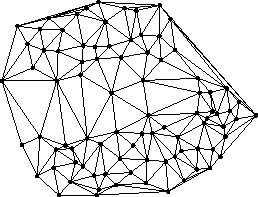
\includegraphics[width=\textwidth]{delaunay-alpha-a}
      \subcaption{Delaunay Triangulation einer beliebigen Punktmenge}
      \label{fig:delaunay-alpha-a}
    \end{subfigure}
    \hfill
    \begin{subfigure}[t]{\subwidth}
      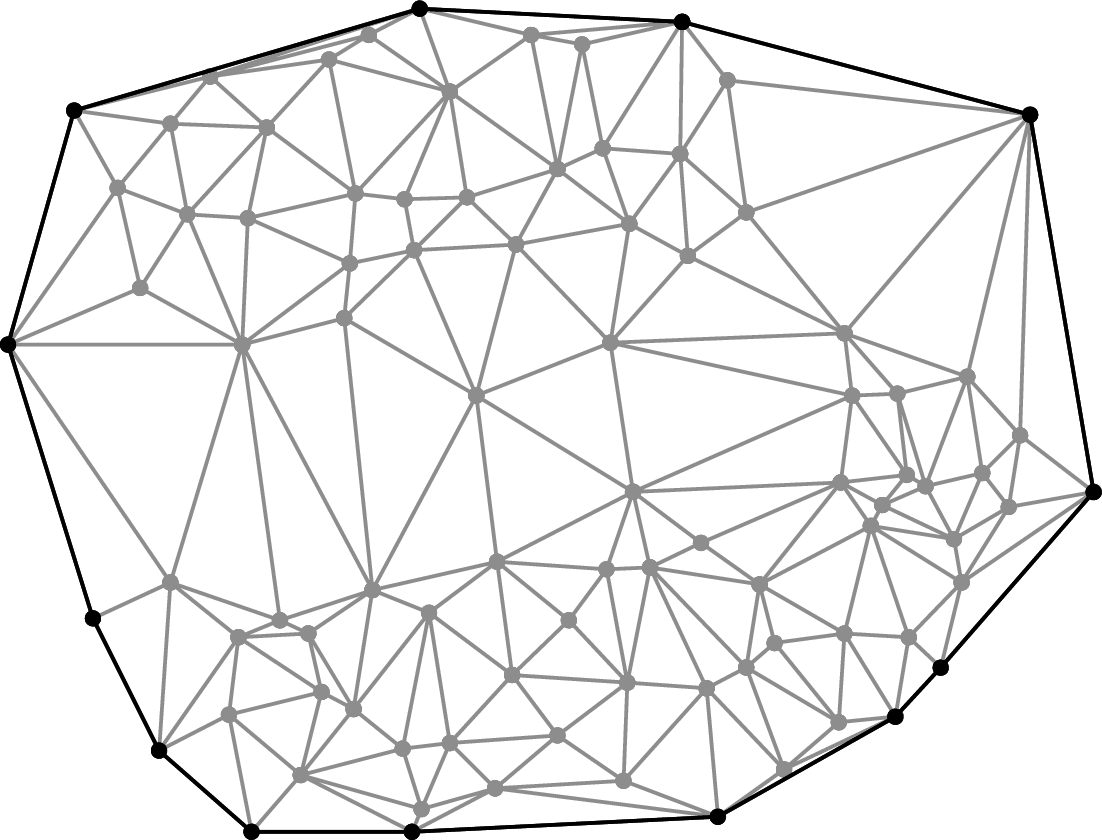
\includegraphics[width=\textwidth]{delaunay-alpha-b}
      \subcaption{Konvexe Hülle: Hülle der Triangulation}
      \label{fig:delaunay-alpha-b}
    \end{subfigure}
  }
  \vspace{2em}
  \captionsetup[subfigure]{singlelinecheck=false}{
    \def\subwidth{0.4\textwidth}
    \def\svgwidth{\textwidth}
    \begin{subfigure}[t]{\subwidth}
      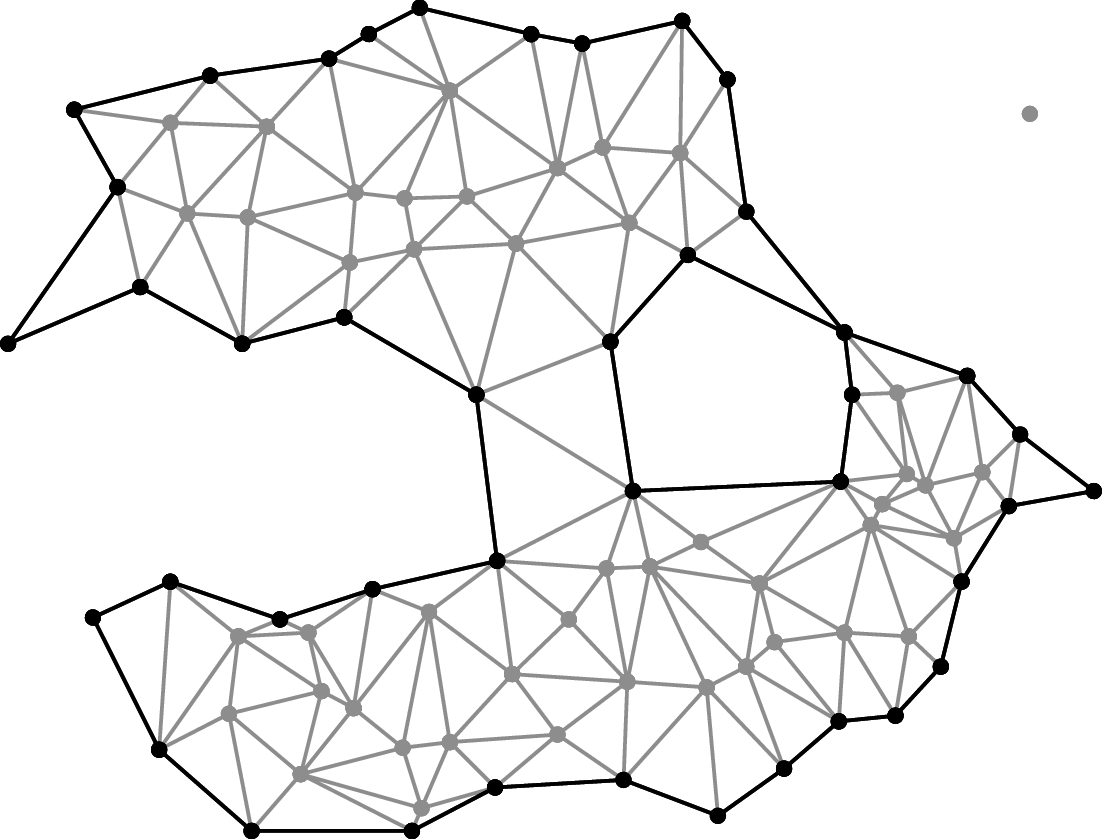
\includegraphics[width=\textwidth]{delaunay-alpha-c}
      \subcaption{Alpha-Form: Hülle nach Entfernung von Simplexen mit $r_d > \alpha$}
      \label{fig:delaunay-alpha-c}
    \end{subfigure}
    \hfill
    \begin{subfigure}[t]{\subwidth}
      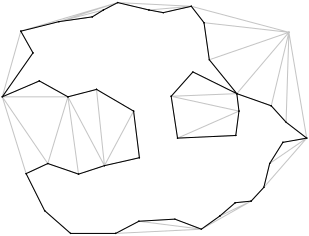
\includegraphics[width=\textwidth]{delaunay-alpha-d}
      \subcaption{Alpha-Form: Hülle nach Entfernung von Simplexen mit $r_d < \alpha$}
      \label{fig:delaunay-alpha-d}
    \end{subfigure}
  }
  \caption[Bestimmung der Oberfläche per Delaunay-Triangulation]{
    Bestimmung der Oberfläche per Delaunay-Triangulation.
    Die Alpha-Form in (d) trianguliert auch Ausreißer-Punkte, zählt sie aber ebenfalls nicht zur Hülle
  }
  \label{fig:delaunay-alpha}
\end{figure}


\cleardoublepage
\cleardoublepage
\chapter{Methoden und Modelle}
%% \chapter{ReaxFF-Potentiale für SiO$_2$-Abscheidungen}

\todo[inline]{Kurze Einleitung}

\section{Stand der Forschung}
\label{present}

Molekulardynamische und kinetische Monte Carlo-Methoden wurden wiederholt zur Simulation von verschiedenen Aspekten von Gasphasenabscheidungen zu Rate gezogen.
Im Folgenden soll ein Überblick über die bisherigen Untersuchungen gegeben werden.
Referenz~\cite{dollet_multiscale_2004} gibt einen Überblick über weitere Multiskalen-Modelle für Gasphasenabscheidungen, welche sich meist auf die Reaktor-Skala beschränken und keine strukturellen Eigenschaften modellieren.

\subsection{Anwendungen von KMC-Simulationen für die Gasphasenabscheidung}

\subsubsection{Dwivedi: gitterbasierte 2D-ALD}

\textsc{V. Dwivedi} und \textsc{A. Adomaitis} haben ein zweidimensionales KMC-Modell für \ce{Al2O3}-ALD entwickelt\cite{dwivedi_multiscale_2009,dwivedi_multiscale_2009-1,dwivedi_multiscale_2010}, um den Gasverbrauch und den GPC-Wert in Abhängigkeit der Partialdrücke der Precursorgase zu ermitteln und in eine Gasflusssimulation zur Kontrolle des Durchmessers von Mikroporen einzubinden.
Dazu werden die Plätze eines hexagonalen Gitters auf die Spezies Sauerstoff, Hydroxyl und Aluminium aufgeteilt, Zustandsübergänge in Abhängigkeit der Besetzung der 6 Nachbarzellen definiert und Übergangsraten ausgehend von den Energiebarrieren der entsprechenden chemischen Reaktionen ermittelt.
Aussagen über die Schichthöhe ergeben sich über die Festlegung des vertikalen Gitterabstandes anhand der Einheitszelle eines \ce{Al2O3}-Kristalles mit anschließender vertikaler Oberflächensuche.

Damit lassen sich zwar GPC-Werte und Precursorverbrauch in Annäherung bestimmen, doch ist durch das zweidimensionale Simulationsgitter keine strukturelle Aussage möglich, obwohl passend gewählte Ereignisse die \ce{Al2O3}-Stöchiometrie erzwingen.
Eigene Untersuchungen des Dwivedi-Modelles resultierten in der Bildung von vertikalen, isolierten \ce{Al-O}-Ketten sowie in der Verstärkung von Kratern und konnten die präsentierten GPC-Werte nicht reproduzieren.

\subsubsection{Mazaleyrat: gitterbasierte 3D-ALD}

Ähnlich zum Dwivedi-Modell nutzt auch das Modell von \textsc{Mazaleyrat et al.}\cite{mazaleyrat_methodology_2005} zur Abscheidungssimulation von Dielektrika auf Silizium-Substraten ein Simulationsgitter, das allerdings in drei Dimensionen definiert ist, auf dem \ce{MgAl2O4}-Spinell-basiert und als Annäherung der eigentlichen Atompositionen verstanden wird.
Durch geschickte Indizierung der Gitterpunkte sind effiziente Wachstumssimulationen von\ce{Al2O3} mit KMC-Methoden möglich, deren strikt kristalline Repräsentation die eigentlich amorphe Struktur nicht darstellen kann
Von den Autoren wurde keine Betrachtung der Rauheit, des Besetzungsgrades der Gitterplätze oder des Wachstumsverhaltens jenseits des dritten Schrittes veröffentlicht.

\subsubsection{Stamatakis: Oberflächen-Reaktionen mit Zacros}

Zwar handelt es sich beim gitterbasierten Zacros-Modell von der Forschergruppe um \textsc{M. Stamatakis}\cite{stamatakis_graph-theoretical_2011,nielsen_parallel_2013,stamatakis_zacros_2014} um eine zweidimensionale Oberflächenbeschreibung für katalytische Reaktionen, doch liegt nahe, seinen effizienten graph-basierten Suchansatz für Ereignisse auch für Gasphasenabscheidungen nutzen zu wollen.
Die Besonderheit von Zacros liegt in einer vereinheitlichten Formulierung der lokalen Zustände und Zustandsübergänge als Teilgraphen des Simulationsgitters, welche effizient durch Algorithmen zum Teilgraphen-Vergleich überprüft werden können.
Ergänzt durch quantenmechanische Simulationen für die Bestimmung der Reaktionsraten ergibt sich ein Werkzeug zur stochastischen Simulation der Reaktionskinetik von Oberflächenprozessen.
%% Aufgrund seiner Formulierung ist aber auch Zacros auf ein periodisches Simulationsgitter begrenzt, welches durch seine Beschreibung als Graph jedoch aus beliebig geformten Einheitszellen bestehen kann.
Die Kombination der in der vorliegenden Arbeit vorgestellten Ansätze mit denen von Zacros ist Gegenstand des derzeit in Beantragung befindlichen EU-Projektes ACCELERATE, einem Konsortium zur ALD-Simulation bestehend aus dem Fraunhofer ENAS, der Gruppe um Stamatakis und weiteren Partnern.

\subsubsection{Clark: Off-Lattice-Simulationen von chemischen Gasphasenabscheidungen}
\textsc{Clark et al.}\cite{clark_hybrid_1996} haben eine Off-Lattice-Methode zur Simulation von Diamantwachstum per CVD entwickelt, die auf der Kombination von KMC- mit Simulated Annealing per Metropolis-Monte-Carlo-Simulationen (MMC), deren Energiewerte mit MD-Berechnungen gewonnen werden.
Dafür wird die lokale Nachbarschaft jedes Adsorptions-Ereignisses unter den Zwangsbedingungen der chemischen Bindungen in MMC-Simu\-la\-tionen relaxiert, während hochfrequente Bewegungen von Wasserstoffatomen durch deren stochastische Verschiebung auf der Oberfläche beschrieben werden.
Damit reduziert sich Simulationszeit, doch müssen mögliche Ereignisse durch in Vorarbeit erforscht werden, statt vom Modell dynamisch erkannt zu werden.

%% Die kombinierte Simulation unterteilt sich in die Betrachtung von hochfrequenten Gleichgewichts-Ereignissen per KMC-Methoden und sowie die Simulation von Adsorptionen und Reaktionen durch MMC-Relaxationen anhand von MD-Kraftfeldern innerhalb der Nachbarschaft.
%% In der ersten Phase des Zyklus' werden hauptsächlich Wasserstoffatome an der Oberfläche durch KMC-Ereignisse verschoben und entsprechend der erwarteten Oberflächenbedeckung ad- und desorbiert.
%% Anschließend werden Precursorfragmente in Form von Methylgruppen an ein Kohlenstoff-Atom an der Oberfläche gebunden und bei konstanter Bindungslänge per MMC-Simulation um dieses rotiert.
%% Zuletzt werden Bindungen zwischen Kohlenstoff-Atomen in der Nachbarschaft des Ereignisortes gebildet, indem sie in einer weiteren MMC-Simulation verschoben werden.

Dieses Modell ist dem im folgenden Abschnitt~\ref{parsivald} vorgestellten Parsivald-Modell in seiner Funktionsweise ähnlich, welches eine thermische Relaxation der Ereignisorte per Molekulardynamik durch, um so freie Atombewegungen an der Oberfläche zu ermöglichen.
%% Eine Erweiterung des Parsivald-Modelles zu MMC-Relaxierungen wäre aber in Zusammenhang mit der Einbindung von Elektronenstrukturrechnungen interessant.

\subsubsection{Biehl: Off-Lattice-KMC von verspannten Kristallen}
In den Veröffentlichungen von \textsc{Biehl et al.}\cite{biehl_off-lattice_2005} wird ein KMC-MD-Hybrid zur zweidimensionalen Off-Lattice-Simulation von Verspannungen in heteroepitaxial gewachsenen Kristallen vorgestellt, der neben Adsorptionsereignissen auch Oberflächendiffusionen betrachtet.
Die Relaxation von Ereignisorten wird bei diesem Modell durch eine nicht näher benannte Energieminimierung der Position einzelner Atome durchgeführt.
Zusätzlich findet in großen zeitlichen Intervallen eine kostspielige globale Energieminimierung statt, die laut der Autoren zur Stabilisierung notwendig ist, obwohl nur kleine Änderungen der Struktur durchgeführt werden.
Da die Anwendung in der Simulation von Kristallen liegt, wurden Lennard-Jones-Potentiale zur Darstellung von Kristallstrukturen gewählt, wodurch sich sehr stabile Strukturen aufgrund der glatten Energielandschaften ergeben.
Damit ist nicht ersichtlich, ob sich diese Methode auch für komplizierte dreidimensionale Strukturen und Kraftfelder eignet.

\subsubsection{Wolf: Transport-Simulationen in der Gasphase}

\textsc{Wolf et al.}\cite{wolf_investigation_2002,wolf_simulation_2010} haben am Zentrum für Mikrotechnologien in Chemnitz in den vergangenen Jahren mit der KMC-Transportsoftware Kalypso\cite{karolewski_kalypso:_2005} die physikalische Gasphasenabscheidung auf der Reaktor-Skala simuliert, um Aussagen über das Schichtwachstum in komplizierten makroskopischen Geometrien zu gewinnen.
Beim Auftreffen eines Atomes an der Oberfläche wird es mit einer Wahrscheinlichkeit, die von der Teilchenenergie und Auftreffwinkel abhängt, adsorbiert oder reflektiert.
Dafür wurde eine Liste zur Interpolation von Wahrscheinlichkeiten vorbereitet, indem das Auftreffen von Atomen an verschiedenen Punkten einer Gitter-Einheitszelle per MD simuliert und anhand der Ergebnisse vieler Simulationen die Wahrscheinlichkeiten bestimmt wurden.
Damit ist diese Methode zur Simulation von epitaktischem Wachstum gut geeignet, beschreibt aber keine rauhen Oberflächen, wie sie bei Gasphasenabscheidung häufig vorliegen\todo{Ref?}.
Der Aufwand für die Vorausberechnung steigt für kompliziertere Oberflächen stark an und ist mit der heutigen Rechenleistung nicht realisierbar.

\subsubsection{Fazit}

KMC-Simulationen werden zur atomistischen Simulation von Gasphasenabscheidungen genutzt, doch sind die Atompositionen häufig auf die Punkte eines Simulationsgitters begrenzt.
Damit können zwar große Simulationsräume effektiv betrachtet werden, doch werden realistische Beschreibungen der oftmals amorphen Materialien verhindert.

Vereinzelt existieren auch atomistische Off-Lattice-Ansätze für KMC-Simulationen, die für die Durchführung von Ereignissen häufig auf molekulardynamische Simulationen zurück greifen.
Diese nutzen meist N-Teilchen-Potentiale in vergleichsweise kleinen Simulationsräumen, wodurch sich amorphe Strukturen oder Oxide nur unzuverlässig beschreiben lassen, doch beschränken sich die untersuchten Arbeiten ohnehin auf kristallines Wachstum oder Verspannungen in Kristallen.

\subsection{Anwendung von MD-Simulationen für die Gasphasenabscheidung}

Molekulardynamische Simulationen werden seit vielen Jahrzehnten zur Bestimmung struktureller und thermodynamischer Eigenschaften verschiedener Materialien eingesetzt, aber nur selten zur Beschreibung von Gasphasenabscheidungen.
Sie lassen sich aber zur Beschreibung von Teilaspekten nutzen, wofür meist durch die Simulation periodischer Strukturen Rückschlüsse auf bestimmte Eigenschaften gezogen werden.

\subsubsection{Gold}
\textsc{Chamati et al.}\cite{chamati_second-moment_2004} haben das thermische Verhalten von Gold-Bulksystemen untersucht, wo hingegen \textsc{Chui et al.}\cite{chui_molecular_2007}, \textsc{Liu et al.}\cite{liu_melting_2001} und \textsc{Shim et al.}\cite{shim_molecular_2003} strukturelle und thermodynamische Eigenschaften von Gold-Nanoclustern betrachtet haben.
Veröffentlichungen zu MD-Simulationen von Aspekten der Gold-PVD finden sich ebenfalls vereinzelt, doch simulieren die meisten den Einschlag von Edelgas-Ionen auf dem Target mit Energien von \SIrange{1}{400}{\kilo\electronvolt}\cite{insepov_molecular_1995,shapiro_simulation_1999} oder tragen komplette Cluster statt einzelner Atome auf\cite{inoue_molecular_2008}.

\subsubsection{Kupfer und Nickel}
Kupfer-Nickel-Multilagensysteme wurden unter anderem von \textsc{Foiles et al.}\cite{foiles_calculation_1985} simuliert, wobei der Einfluss der Sputterenergie der Atome auf die Rauheit der abgeschiedenen Oberflächen und Schichten hauptsächlich von \textsc{Zhou et al.}\cite{zhou_atomistic_1998} untersucht wurde.
Der durch unterschiedliche Bindungslängen entstehende Versatz zwischen den Kupfer- und Nickel-Kristallen wurde von \textsc{Rao et al.}\cite{rao_atomistic_2000} simuliert.

\subsubsection{Silizium}
Für Silizium finden sich thermodynamische Expansions-Simulationen von \textsc{Buda et al.}\cite{buda_thermal_1990} sowie Untersuchungen von \textsc{Insepov et al.}\cite{insepov_molecular_1995} zur Auswirkung von gerichteten Cluster-Ein/-schlägen in Abhängigkeit der Einschlagsenergie.
\textsc{Torre et al.}\cite{torre_study_2002} haben außerdem die Oxidierung von Silizium-Nanopartikeln mit Drei-Teilchen-Potentialen simuliert.
%% {mehr! PVD und Oxidation / Hydroxylierung von Oberflächen} - Gibt's nicht

\subsubsection{Aluminiumoxid}
Für amorphe und kristalline \ce{Al2O3}-Bulksysteme finden sich Simulationsergebnisse von \textsc{Alvarez et al.}\cite{alvarez_computer_1995,alvarez_molecular_1992} und von \textsc{Gutierrez et al.}\cite{gutierrez_molecular_2002} sowie für \ce{Al2O3}-Oberflächen von \textsc{Adiga et al.}\cite{adiga_atomistic_2006}.
Sowohl Schmelzen als auch amorphes \ce{Al2O3} wurden unter anderem von \textsc{Gutierrez et al.}\cite{gutierrez_structural_2000} und \textsc{Vashishta et al.}\cite{vashishta_interaction_2008} simuliert.
\textsc{Russo et al.}\cite{russo_molecular_2011} haben erfolgreich Oberflächen-Reaktionen zwischen einem Aluminium-Cluster und Wassermolekülen unter Nutzung der ReaxFF-Formulierung simuliert, während \textsc{Puri et al.}\cite{puri_thermo-mechanical_2010} das Schmelz- und Diffusionsverhalten von \ce{Al2O3}-ummantelten \ce{Al}-Nanopartikeln untersuchten.
Diese Vielfalt an Simulationen zeigt sich jedoch nicht in der Zahl der veröffentlichten Potentialparametrisierungen, von denen nur eine kleine Zahl für \ce{Al2O3}-Simulationen zur Verfügung stehen.

\subsubsection{Fazit}
Die Untersuchungen von Gasphasenabscheidungsprozessen mittels Molekulardynamik beschränken sich aufgrund der langen Relaxationszeiten und des Rechenaufwandes unter Nutzung reaktiver Kraftfelder.
Wenige Untersuchungen simulieren deshalb mehr als \num{50000} Atome, weshalb sich besonders bei der Bestimmung struktureller Eigenschaften Finite Size-Effekte bemerkbar machen können.
Darüber hinaus werden einige der genutzten Potentialparametrisierungen nicht veröffentlicht, wodurch die entsprechenden Ergebnisse nicht reproduzierbar oder auf andere Probleme übertragbar sind.
Dem steht die Vielzahl von verschiedenen Parametrisierungen gegenüber, von denen jede einzelne nur auf ein spezielles Problem anwendbar ist.
Eine Suche nach EAM-Kraftfeldern für Kupferatome in der Potentialdatenbank des NIST\cite{becker_interatomic_2014} ergibt beispielsweise eine zweistellige Zahl an Kupfer-Parametrisierungen, die einzeln hinsichtlich eigener Problemstellungen überprüft werden müssen (Abschnitt~\ref{copperpvd}).

\clearpage
\section{Parsivald-Modell}
\label{parsivald}

Parsivald (Parallel Atomistic Reaction Simulator for Vapor and Atomic Layer Depositions) entstand 2012 als namenloses Resultat meiner Bachelorarbeit\cite{lorenz_entwicklung_2012} am Fraunhofer ENAS mit dem Ziel der Simulation von Atom\-lagen\-abscheidungs-Prozessen.
Das Programm war beschränkt auf die atomistische Simulation von Metall\-oxid-ALD mittels MEAM-Potentialen, die in dieser Arbeit auf PVD und CVD mit beliebigen Potentialen erweitert wurde.

\subsection{Zielsetzung für Parsivald}

Das vorgestellte Parsivald-Modell vereint die Stärken von MD- und KMC-Methoden, um so Gasphasenabscheidungen in großen Simulationsräumen mit atomistischer Genauigkeit zu simulieren.
Ein wesentliches Ziel ist, die strukturellen Eigenschaften der abgeschiedenen Schichten auch für große Oberflächen in effizienten Rechnungen gut wiederzugeben.
Dabei soll nicht nur die Untersuchung flächiger Abscheidungen sondern auch die Untersuchung des Wachstums an beziehungsweise in dreidimensionalen Nanostrukturen, wie etwa Stufen, Gräben und Poren ermöglicht werden.
Dazu müssen relativ große Strukturen von \SI{10x10}{\nano\meter} bis \SI{1x1}{\micro\meter} und Schichtdicken bis zu \SI{20}{\nano\meter} (\num{200} ALD-Zyklen) in akzeptabler Rechenzeit (einige Tage bis wenige Wochen) simuliert werden können.
Die Simulationsräume enthalten dann bis zu \num{1e9} Atome, liegen also bis zu \num{5} Größenordnungen über den Möglichkeiten reiner MD-Simulationen.
Durch die Nutzung massiver Parallelisierung werden zudem atomistische Simulationen über eine Simulationszeit von mehreren Minuten ermöglicht.

\subsection{Beschreibung}

\begin{figure}[b]
  \centering
  \def\svgwidth{\textwidth}
  \input{img/parsivald-schema-flat.pdf_tex}
  \caption{Auswahl und Durchführung einer Adsorption, verteilt auf KMC und MD}
  \label{fig:parsivald-schema}
\end{figure}

Der Grundgedanke von Parsivald besteht in der Aufteilung der Simulation in mehrere Skalen.
So ergeben sich zwei zeitliche Skalen durch die hohe Geschwindigkeit der Adsorptionen im Kontrast zu der niedrigen Frequenz, in der diese in direkter Nachbarschaft auftreten.
Einzelne Adsorptionen werden durch KMC-Ereignisse dargestellt, in welchen die Nachbarschaft des Adsorptionsortes (MD-Box) aus der globalen Struktur extrahiert, einem MD-Prozess zur Berechnung übergeben und anschließend wieder in die globale Struktur zurückgeführt wird (Abbildung~\ref{fig:parsivald-schema}).
Die MD-Simulation führt in der Regel eine Relaxierung der Oberfläche im kanonischen Ensemble durch, doch sind auch Strukturoptimierungen möglich.

\begin{figure}
  \centering
  \def\svgwidth{\textwidth}
  \input{img/parsivald-stephierarchy.pdf_tex}
  \caption[Funktionsweise des Parsivald-Programmes]{
    Funktionsweise des Parsivald-Programmes.
    Event-Typen unterscheiden sich durch die MD-Simulation (Relaxation, Reaktion) oder das Precursorgas.\\
    Siehe auch Abbildung~\ref{fig:parsivald-modes}.
  }
  \label{fig:parsivald-stephierarchy}
\end{figure}

Abbildung~\ref{fig:parsivald-stephierarchy} stellt die Funktionsweise einer gesamten Parsivald-Simulation vor, die im Wesentlichen aus Vor- und Nachbereitung sowie einer Prozessschleife besteht, in der nacheinander komplette KMC-Simulationen (Parsivald-Schritte) durchgeführt werden.
Innerhalb der Parsivald-Schritte werden mögliche Adsorptionen, Ligandenaustausch-Reaktionen oder Relaxationen als KMC-Ereignisse verwaltet, welche auf eine dünne Oberflächenschicht begrenzt sind.
Nach jedem Ereignis wird eine rechenaufwendige Konnektivitätsprüfung an den Ereignisorten durchgeführt, um desorbierte Atome zu erkennen und von der Oberfläche auszuschließen.
Damit werden Diffusionen in das Material oder auf seiner Oberfläche unterbunden, dafür jedoch eine effiziente Host-Worker-Parallelisierung ermöglicht.
%%Ereignisse mit überlappenden MD-Boxen werden in Warteschlangen verwaltet, um die Reihenfolge der KMC-Ereignisse zu bewahren.

Als Eingaben der Simulation dienen das Substrat, eine Sammlung verschiedener Prozessparameter wie Prozesstemperaturen, Expositionszeiten und Abscheidungsmodi (Abbildung~\ref{fig:parsivald-modes}), MD-Befehlslisten mit Platzhaltern (MD-Masken) sowie die Potentialparametrisierung.
In die MD-Masken werden im Verlauf der Simulation die Eigenschaften der Ereignisse eingetragen, bevor sie als Steuerbefehle an die MD-Simulationen übergeben werden.
Die Ausgabe erfolgt kontinuierlich in Ereignis-Logs sowie nach jedem Parsivald-Schritt in einem atomistischen Dateiformat, über das strukturelle Eigenschaften bestimmt werden können.

Eine typische Abscheidungs-Simulation verläuft nach folgendem Schema:
Zuerst wird das Substrat aus einer Datei gelesen und periodisch auf die Größe des Simulationsraums erweitert.
Das Substrat muss xy-periodische Anschlussbedingungen und eine Mindesthöhe entsprechend der Größe der MD-Box erfüllen und stabil gegenüber den genutzten MD-Potentialen sein.
Es lassen sich ansonsten beliebig gemischte und strukturierte Substrate verwenden.
Pro Precursorart und Schritt (Halbzyklus für ALD) wird eine Ereignismaske vorbereitet, welche die physikalischen und numerischen Parameter inklusive der MD-Masken beinhaltet.
Anschließend beginnt die Hauptschleife mit dem ersten Parsivald-Schritt, in dem mögliche Ereignisse auf der Oberfläche gesucht werden, die vom KMC-Algorithmus nacheinander ausgewählt und von MD-Workern möglichst parallel simuliert werden.
Bei Erreichen der vorgegebenen Simulationszeit startet der nächste Schritt im Zyklus.
Die Abscheidungssimulation endet nach einer vorgegebenen Anzahl von Zyklen oder bei vollständiger Füllung des Simulationsraumes mit Atomen.

Mit diesem Schema lassen sich auch CVD- und PVD-Prozesse simulieren, indem der Zyklus dem zu simulierenden Prozesse angepasst wird (Abbildung~\ref{fig:parsivald-modes}).
%%auf einen einzigen Schritt beschränkt wird und bei CVD-Simulationen mehrere Arten von Ereignissen gleichzeitig betrachtet.
%%Der Zyklen-Timeout kann dann zur Kontrolle der Ausgabefrequenz atomistischer Strukturen genutzt werden.
Die Ereignisraten ergeben sich für PVD-Prozesse aus der Adsorptionsrate der Atome auf der Oberfläche, für CVD und ALD hingegen aus der Arrhenius-Gleichung.
%% Für ALD und CVD lässt sich die Wachstumsrate aus der Reaktionskinetik abschätzen, während sie bei PVD-Simulationen durch den entsprechenden Prozessparameter festgelegt wird.

\begin{figure}[hbp]
  \captionsetup[subfigure]{singlelinecheck=false}
  \begin{subfigure}[t]{5.7cm}
    \def\svgwidth{\textwidth}
    \input{img/parsivald-modes-ald.pdf_tex}
    \subcaption{ALD-Modus}
  \end{subfigure}
  \hfill
  \begin{subfigure}[t]{4.7cm}
    \def\svgwidth{\textwidth}
    \input{img/parsivald-modes-cvd.pdf_tex}
    \subcaption{CVD-Modus}
  \end{subfigure}
  \hfill
  \begin{subfigure}[t]{3cm}
    \def\svgwidth{\textwidth}
    \input{img/parsivald-modes-pvd.pdf_tex}
    \subcaption{PVD-Modus}
  \end{subfigure}
  \caption[Prozesszyklen für ALD, CVD und PVD]{
    Prozesszyklen für ALD, CVD und PVD.
    Atomistische und statistische Ausgaben erfolgen nach jedem Schritt.
    ALD (a) nutzt einen Schritt pro Halbzyklus.
  }
  \label{fig:parsivald-modes}
\end{figure}

\subsection{Annahmen und Einschränkungen}

Die folgenden Annahmen werden getroffen, um stabile Prozesse mit guter Skalierbarkeit auf großen Zeit- und Raumskalen beschreiben zu können:

\begin{enumerate}
\setlength\itemsep{0ex}
\item Alle Ereignisse finden auf der Oberfläche statt
\item Ereignisse sind zeitlich und räumlich getrennt
\item Oberflächendiffusion ist vernachlässigbar
\item Bulkdiffusion ist vernachlässigbar
\end{enumerate}

Die Beschränkung des Modelles auf diffusionsarme Oberflächenabscheidungen ergibt sich aus der Notwendigkeit, Bereiche des Simulationsraumes im statischen Gleichgewicht, in dem keine Ereignisse statt finden, zugunsten der Rechenzeit bei der MD-Simulation zu vernachlässigen.
Das betrifft die Gasphase und den größten Teil des Bulkmateriales ebenso wie abgeschirmte Bereiche der Oberfläche.
Für Prozesse, welche die oben aufgelisteten Annahmen nicht unterstützen, degeneriert Parsivald zu einer reinen MD-Simulation mit enormem Overhead.
Ein beschränktes Maß an Oberflächendiffusion lässt sich zwar mit längeren Relaxationszeiten und separaten Relaxations-Ereignissen behandeln, allerdings kann aufgrund der begrenzten Größe der MD-Boxen nur die Diffusion weniger Atome behandelt werden kann.

Weiterhin ist Parsivald auf die zugrunde liegende Molekulardynamik beschränkt.
So lassen sich nur Systeme simulieren, für die Potentialparametrisierungen existieren, die sowohl Bulksysteme als auch Oberflächen darstellen können, wie es bei EAM- und vielen ReaxFF-Potentialen der Fall ist.
ReaxFF-Potentiale sind um mehrere Größenordnungen rechenaufwendiger als EAM-Potentiale, welche in gleichem Maße rechenaufwendiger als Paarpotentiale sind, weshalb große Systeme nicht mehr mit reiner Molekulardynamik berechenbar sind und sich die Effizienz von Parsivald bemerkbar macht.

Werden zusätzlich Moleküle und deren Reaktionen mit Oberflächenliganden dargestellt, lassen sich Precursor-Oberflächen-Reaktionen direkt in Parsivald simulieren.
Andernfalls muss der Precursor über sein abzuscheidendes Zentralatom und zusätzliche Mechanismen wie explizite sterische Hinderung angenähert werden.
Die Suche nach Ereignisorten würde dann über exponierte Oberflächenatome und Revisionslisten statt über Oberflächenliganden angenähert.
Eine tatsächliche Anwendbarkeit beider Methoden muss für jeden Prozess einzeln abgeschätzt werden, da die nun fehlenden Precursorliganden strukturell entscheidend für den Aufbau der abgeschiedenen Schicht sein können.

\subsection{Erweiterungen im Rahmen der Masterarbeit}

Mit der vorliegenden Arbeit wurde das Parsivald-Modell und seine Implementierung um PVD- und CVD-Modi (Abbildung~\ref{fig:parsivald-modes}), eventgebundene sterische Hinderung zum Zweck der CVD-Simu\-lation, ein allgemeines Konfigurationsformat und allgemeine MD-Masken erweitert.
Intern kam die Unterstützung verschiedener atomistischer Dateiformate, die Einbettung der LAMMPS-Umgebungs\-variablen zur Potentialsuche, globale und lokale Suchpfade für alle Eingabedateien und ein interner sowie beliebig viele externe Workerpools dazu.
Ein standardisiertes Buildsystem sorgt für schnelle und sichere Kompilierung der Software, und eine Vielzahl externer Werkzeuge zur Vorbereitung und Analyse von Prozessen (Anhang~\ref{appendix_tools}) ermöglicht schnelle Zyklen der Parameteroptimierung und Auswertung.

Diese Änderungen ermöglichen eine einfachere Vorbereitung, Simulation und Untersuchung verschiedener Prozesse und eine aussagekräftigere Analyse der Ergebnisse.
Auch eine automatisierte Optimierung der Simulation durch selbstständige Anpassung der Prozessparameter wie Temperatur, Druck und Expositionszeit oder MD-spezifischer Parameter wie Thermostatdämpfung, Relaxationsdauer oder Zeitschrittweite ist mittels des Konfigurationsmechanismus' denkbar.

%% Zusätzlicher Aufwand musste beim Einkapseln der MD-Bibliothek LAMMPS betrieben werden (Abschnitt~\ref{lammpssucks}).

\subsection{Behandlung von fehlerhaften Ereignissen}

Parsivald-Simulationsläufe geben neben der atomistischen Struktur verschiedene Statistiken und Werte in Form von Daten- und Logdateien aus.
Das beinhaltet die Zahl der versuchten, erfolgreichen und fehlgeschlagenen Ereignisse, laufende Worker, überlagerte und deshalb zurückgestellte Ereignisse und die Anzahl aller Atome.
Optional lässt sich eine Verteilung der Häufigkeit eines Zugriffes auf Positionen in der xy-Ebene angeben, um bei reaktiven Prozessen die Auswahlkriterien von Ereignisorten zu prüfen.
Anhand der atomistischen Struktur lassen sich Oberflächenrauheiten, Porenverteilungen, Dichten, Schichtdicken und Eigenschaften eventueller Kristalle bestimmen (Abschnitt~\ref{mdmethods}).

Die Auswertung der Abbruchrate, also des Verhältnisses von fehlgeschlagenen Ereignissen zu versuchten Ereignissen, ist besonders bei der Optimierung von Prozessparametern wichtig, da sich über sie Fehler in der Prozesskonfiguration oder in der gebildeten Struktur frühzeitig erkennen lassen.
Ein Abbruch ist dabei eine MD-Simulation, die abstürzt, ihre Zeitbegrenzung erreicht oder zur Desorption von Atomen und Molekülen führt.
Da die LAMMPS-Bibliothek mit einer geringen Wahrscheinlichkeit unvorhergesehen und ohne Fehlernachrichten abstürzen kann, obwohl die Simulation selbst erfolgreich verlaufen wäre, werden fehlgeschlagene MD-Boxen einem zweiten Prozess zur Simulation übergeben.
Schlägt auch diese fehl, liegt mit hoher Wahrscheinlichkeit ein struktureller oder methodischer Fehler vor.
In der aktuellen Implementierung gitl das Herausschlagen von Atomen aus der Oberfläche, wie es bei Sputter-Prozessen statt finden kann, als Abbruch, weshalb in der vorliegenden Arbeit geringe Teilchenenergien oder schnelle Thermostatdämpfungen eingesetzt werden.

Da bei Abbrüchen bereits ausgewählte Ereignisse verworfen und somit die Abscheidungsraten leicht unterschätzt werden, müssen die Ereignisraten dynamisch entsprechend der mittleren oder erwarteten Abbruchrate angepasst werden.
Für CVD-Simulationen ist eine Anpassung der Ereignisraten in der Regel nicht notwendig, da fehlerhafte MD-Ereignisse auf eine versehentliche Auswahl eines Ereignisortes zurück zu führen sind.
Die Auswahlkriterien der Ereignisorte sollten alle potentiellen Ereignisse beinhalten, wobei einige weitere Orte versehentlich ausgewählt werden können, die keine Adsorptionen zulassen.
Eine präzisere Beschreibung der Nachbarschaft und des Bindungszustandes eines Atomes könnte helfen, die Auswahlkriterien zu präzisieren.
Bisherige Parsivald-Simulationen zeigen Abbruchraten von \SI{<1}{\percent} für stabile Prozesse, wo hingegen fehlerhaft eingestellte Simulationen Werte \SI{>10}{\percent} aufweisen.

\clearpage
\section{Tests für MD-Potentiale zur Schichtabscheidung}

Vor der Nutzung von Parametrisierungen von Wechselwirkungspotentialen für die Molekulardynamik sollten diese durch eine Reihe von Tests auf ihre Anwendbarkeit geprüft werden.
Diese Parametrisierungen sind jeweils für einen speziellen Zweck erstellt worden und decken meist nur diesen zuverlässig ab\todo{und manchmal nicht mal das}.
Das bedeutet einerseits, dass man Potentiale, die auf thermodynamische Probleme optimiert sind, nur selten zur Simulation struktureller Eigenschaften nutzen kann, und umgekehrt.
Andererseits stehen hinter jeder Parametrisierung besondere Zielsetzungen, die oft vom eigenen Einsatzgebiet abweichen und eigentlich eine Anpassung der Parametrisierung, mindestens jedoch ihre Prüfung zur Voraussetzung haben.
So unterstützen Potentiale zur Darstellung von Molekülen häufig keine Bulks und Oberflächen, und umgekehrt.

Dem Thema der Arbeit entsprechend, sollen die zu untersuchenden Systeme strukturelle und chemische Eigenschaften in beschränkten Temperaturbereichen darstellen, was sich auch in den Tests zeigt.
So wird die kristalline und amorphe Struktur, ihre Dichte, radiale Verteilungsfunktion, Bindungslängen und Koordination einerseits untersucht, und die Darstellbarkeit der zugrunde liegenden Reaktionen per ReaxFF-Formulierung sowie die Diffusion eines Atomes auf der Oberfläche andererseits.
Diese Tests sind in Tabelle \ref{tab:mdtestvariants} dargestellt.

\begin{table}
  \rowcolors{0}{white}{lightgray}
  \begin{tabularx}{\textwidth}{|lXX|}
    \hline
    \textbf{Test} & \textbf{Vorgehensweise} & \textbf{Ergebnis} \\
    \hline
    Kristall-Strukturoptimierung & LAMMPS minimize & Dichte, RDF, Koordination, Bindungslänge \\
    Kristall-Relaxation & LAMMPS nvt/npt run & Dichte, RDF, Koordination, Bindungslänge \\
    Oberflächen-Relaxierung & Relaxierung einer nichtperiodischen Struktur in unbegrenztem Raum  & Oberflächenstabilität bei geringem Druck \\
    Präparation amorpher Struktur & zufällige Atompositionen, Relaxation bei hohen Temperaturen, Abkühlung & Dichte, Koordination, Hauptbindungslänge \\
    Precursor-Simulation & LAMMPS nvt run jedes Precursormoleküles & Stabilität \\
    Precursor-Reaktionen & LAMMPS nvt run beider Precursormoleküle & Reaktivität, Stabilität \\
    Oberflächen-Reaktionen & Reaktion eines Moleküles mit einer präparierten Oberfläche & Reaktivität, Diffusionsgrad \\
    Parsivald-Simulation & Komplette Abscheidungs-Simulation mit Parsivald & Anwendbarkeit \\
    \hline
  \end{tabularx}
  \caption[asd]{dsa mit LAMMPS, Präparation mit Materials Studio}
  \label{tab:mdtestvariants}
\end{table}


\cleardoublepage
\chapter{Simulationen von Gasphasenabscheidungen}
\label{results}

Unter Nutzung der in Kapitel~\ref{theory} und Kapitel~\ref{models} vorgestellten Methoden werden im folgenden Kapitel Abscheidungen mit dem Ziel simuliert, die Präparation und Durchführung von unterschiedlichen Abscheidungsprozessen mit Parsivald zu untersuchen und Einschränkungen des Parsivald-Modelles für PVD und CVD zu prüfen.

Dazu werden verschiedene Systeme auf unterschiedliche Aspekte von Gas\-phasen\-abschei\-dungs-Simu\-la\-tionen mit dem Parsivald-Modell untersucht:
Abschnitt~\ref{goldpvd} zeigt anhand von Gold-PVD allgemeine Voruntersuchungen eines Parametersatzes, strukturelle Unterschiede zwischen realen und simulierten per PVD abgeschiedenen Schichten, die Simulation von Schichtabscheidungen auf strukturierten Substraten sowie einen Vergleich der Laufzeitgrößen mit theoretischen Werten.
Im anschließenden Abschnitt~\ref{copperpvd} werden Voruntersuchungen unterschiedlicher Parametersätze, die Bildung von Unebenheiten an der Oberfläche und deren automatische Schließung in der Parsivald-Simulation anhand von Kupfer-PVD vorgestellt.
Danach werden Kupfer-Nickel-Multi\-lagen\-systeme in Abschnitt~\ref{multilayer} mit Parsivald simuliert und die Ergebnisse mit denen reiner MD-Simulationen verglichen.
In Abschnitt~\ref{siliconpvd} werden dann Silizium-PVD-Systeme mit dem Ziel der Abscheidung nichtmetallischer Schichten auf Porösität und Wachstum amorpher Strukturen untersucht.
Zuletzt kehrt Abschnitt~\ref{aluminaald} kurz zum Thema der Bachelorarbeit zurück und untersucht mit MD-Methoden die Stabilität von TMA und Wasser als Precursoren der \ce{Al2O3}-ALD sowie die Hydroxylierung einer Aluminiumoxid-Oberfläche durch Wassermoleküle.

\iftestonly
\else
  \section{Gold-PVD}
\label{goldpvd}

Als Testsystem für PVD-Prozesse bietet sich Gold-PVD an, die zwar durch Oberflächendiffusion dominiert wird, jedoch ideale fcc-kristalline Strukturen bildet.
Die genutzte EAM-Potentialdatei stammt aus dem \todo{ref}LAMMPS-Paket, basiert aber auf Parametern von Foiles et al.\cite{foiles_embedded-atom-method_1986}, die für Einbettung einzelner Atome in Bulk- und Oberflächensysteme optimiert wurden.

\subsection{Voruntersuchungen}

Zur Validierung grundlegender Materialeigenschaften wurden Bindungslängen, Dichten und Koordinationszahlen aus einer relaxierten kristallinen Phase untersucht (Tabelle \ref{tab:goldpreresults}).
Zur Bestimmung dieser Werte wurde ein Goldkristall von \SI{40x40x40}{\angstrom} Größe auf \SI{1000}{\kelvin} aufgeheizt, im kanonischen Ensemble relaxiert und anschließend abgekühlt.
Wie man den Ergebnissen ansehen kann, bleibt die Kristallstruktur erwartungsgemäß erhalten (die Schmelztemperatur wurde für die Relaxierung nicht überschritten) und steht in guter Übereinstimmung mit Literaturwerten.
Die Parametrisierung repräsentiert somit das Zielsystem.

\begin{table}
  %% \oddrowcolors
  \caption[Eigenschaften von Gold]{Vergleich der Eigenschaften von Gold mit experimentellen und Literaturdaten als Voruntersuchung des PVD-Prozesses
    %% \todo[inline]{ref}
  }
  \label{tab:goldpreresults}
  \begin{tabularx}{\textwidth}{|lXXXX|}
    \hline
    \textbf{unters. Größe} & \textbf{Temperatur} & \textbf{Simulation} & \textbf{Experiment} & \textbf{Abweichung}\\
    \hline
    Bindungslänge  &  \SI{50}{\kelvin}   &  \SI{2.885}{\angstrom}                    &  \SI{2.884}{\angstrom}                    &  \SI{0.05}{\percent}  \\
    Koordination   &  \SI{50}{\kelvin}   &  \SI{12.00}{}                             &  \SI{12.00}{}                             &  \SI{0}{\percent}     \\
    Dichte         &  \SI{300}{\kelvin}  &  \SI{18.99}{\gram\per\cubic\centi\meter}  &  \SI{19.30}{\gram\per\cubic\centi\meter}  &  \SI{1.6}{\percent}   \\
    Dichte         &  \SI{500}{\kelvin}  &  \SI{18.89}{\gram\per\cubic\centi\meter}  &  \SI{19.13}{\gram\per\cubic\centi\meter}  &  \SI{1.2}{\percent}   \\
    \hline
  \end{tabularx}
\end{table}

%% \todo[inline]{Oberflächenvalidierung}

\subsection{Thermodynamische Eigenschaften}
\label{goldthermo}

Neben strukturellen Eigenschaften bilden EAM-Potentiale auch einige thermodynamische Eigenschaften von Metallen ab.
Für deren Untersuchung wurde die Massendichte in Abhängigkeit der Temperatur für die Teststruktur aufgenommen, die langsam auf \SI{2000}{\kelvin}, also weit über den Schmelzpunkt von \SI{1337}{\kelvin}, aufgeheizt wurde.
Die Ergebnisse (Abbildung \ref{fig:goldthermo}) zeigen gute Übereinstimmung mit experimentellen Daten, wofür Relaxationszeiten $t_\text{relax}$ oberhalb von \SI{20}{\pico\second} und Thermostat-Dämpfungsparameter $D_T$ \SI{\approx0.02}{\femto\second} als notwendig ermittelt wurden.
Bei geringeren $t_\text{relax}$ oder $D_T$ relaxiert das System innerhalb eines Temperaturschrittes nicht vollständig, wodurch der Schmelzpunkt überschätzt wird, wie in Abbildung \ref{fig:goldthermo-b} zu sehen ist.

\begin{figure}
  \captionsetup[subfigure]{singlelinecheck=false}
  \def\subfigwidth{7cm}
  \begin{subfigure}[t]{\subfigwidth}
    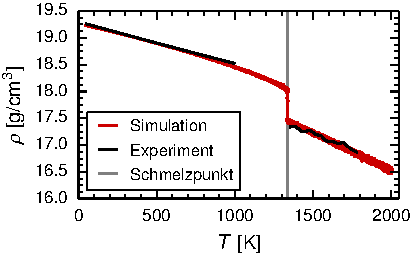
\includegraphics[width=\textwidth]{gold_bestthermo}
    \subcaption{Temperaturverlauf bei $ t_\text{relax}=\SI{50}{\pico\second}$ und $D_T=\SI{0.02}{\femto\second}$}
    \label{fig:goldthermo-a}
  \end{subfigure}
  \hfill
  \begin{subfigure}[t]{\subfigwidth}
    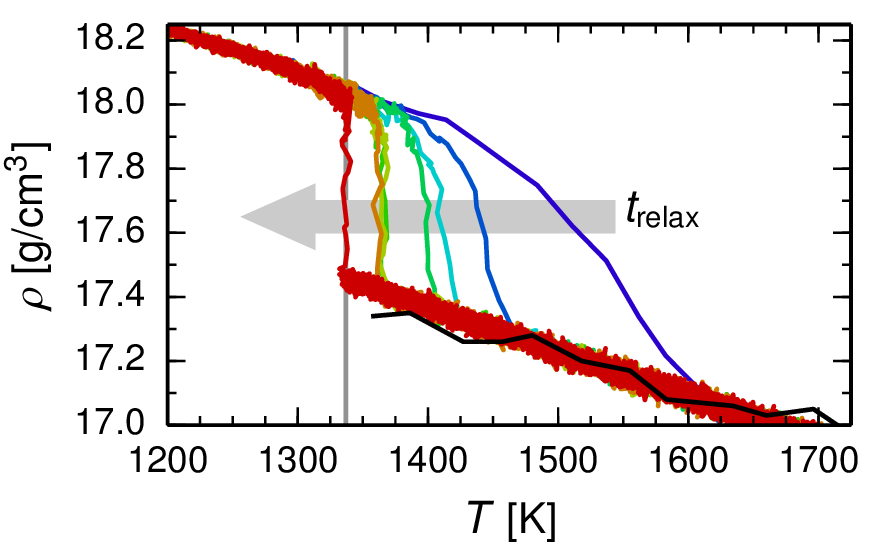
\includegraphics[width=\textwidth]{gold_relaxtime}
    \subcaption{Abhängigkeit des simulierten Schmelzpunktes von der Relaxationszeit}
    \label{fig:goldthermo-b}
  \end{subfigure}
  \caption[Ergebnisse thermodynamischer Simulationen von Gold]{Ergebnisse thermodynamischer Simulationen von Gold.
    Verlauf stimmt gut mit experimentellen Daten (schwarze Linien) überein.
    Experimentelle Werte stammen aus Standardliteratur sowie von Brillo et al.\cite{brillo_density_2006}.
  }
  \label{fig:goldthermo}
\end{figure}

\subsection{Prozess-Simulation}

Zur Simulation eines Gold-PVD-Prozesses mit Parsivald wurden die untersuchten Potentialparameter sowie ein Kristallsubstrat im PVD-Modus eingelesen und Relaxationszeiten und Größen der MD-Simulationsräume aus den Vorbetrachtungen übernommen.
Damit ergeben sich Reaktionsräume der Größe \SI{37x37x25}{\angstrom} mit jeweils ca. \num{1800} Atomen, Relaxationszeiten von \SI{1.4}{\nano\second} in \num{1400} Simulationsschritten und Auftreffgeschwindigkeiten von \SI{4}{\angstrom/\pico\second}, die aus üblichen Sputterbedingungen stammen.\todo{wie berechnet?}

Abbildung \ref{fig:golddepositions-a} zeigt, wie das Substrat unter Erhalt der Kristallstruktur fortgesetzt wird.
Poren und Einschlüsse wurden durch Untersuchung der Alphastruktur nicht gefunden.
Abbildung \ref{fig:goldroughness-a} stellt die Rauheit dar, die beim glatten Substrat über den Abscheidungszeitraum konstant geblieben ist.
Fehler- und Abbruchraten bei den LAMMPS-Berechnungen lagen mit \SI{0.25}{\percent} unterhalb des aus den ALD-Prozessen der Bachelorarbeit erwarteten Wertes von \SI{5}{\percent}

\subsubsection{Wachstum auf strukturierten Substraten}

Neben dem glatten Substrat wurden auch Abscheidungen auf strukturierten Substraten (Abbildung \ref{fig:golddepositions}) mit den gleichbleibenden Prozessbedingungen simuliert.
Als Substrate wurden Stufen oder Spitzen mit einer Höhe von jeweils \SI{20}{\angstrom} und Neigungen von \SI{15}{\degree}, \SI{20}{\degree}, \SI{30}{\degree}, \SI{45}{\degree}, \SI{60}{\degree} und \SI{90}{\degree} präpariert.
Auf vorherige Relaxierung der Substrate wurde aufgrund der Prozessstabilität sowie der relaxierenden Eigenschaften der MD-Ereignisse verzichtet.
Zusätzlich wurden Lamellen und Gitter mit einer Strukturbreite von \SI{16}{\angstrom} zur Untersuchung eventueller Prozessartefakte präpariert.

\begin{figure}
  \captionsetup[subfigure]{singlelinecheck=false}
  \def\subfigwidth{0.31\textwidth}
  \begin{subfigure}[t]{\subfigwidth}
    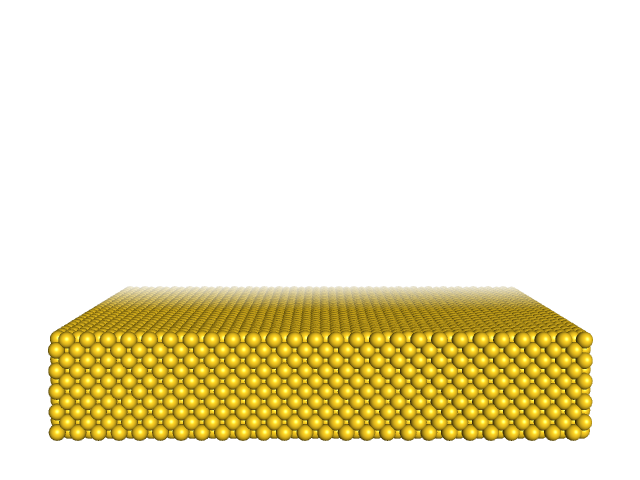
\includegraphics[width=\textwidth]{Au_substrate_flat}
    \subcaption{Glattes Gold-Substrat}
    \label{fig:golddepositions-a}
  \end{subfigure}
  \hfill
  \begin{subfigure}[t]{\subfigwidth}
    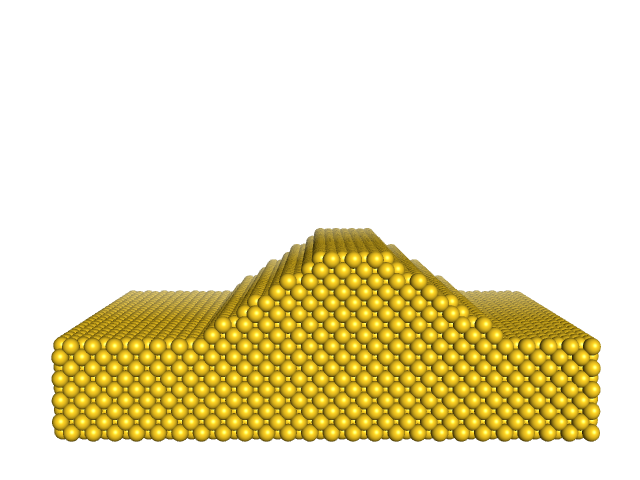
\includegraphics[width=\textwidth]{Au_substrate_step30}
    \subcaption{Gold-Stufe, \SI{30}{\degree}}
    \label{fig:golddepositions-b}
  \end{subfigure}
  \hfill
  \begin{subfigure}[t]{\subfigwidth}
    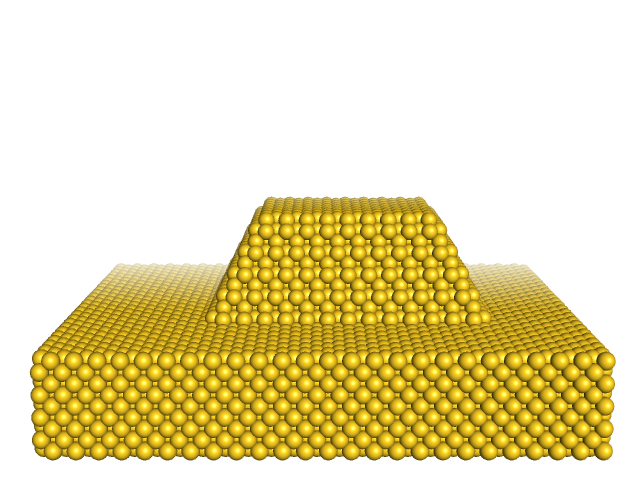
\includegraphics[width=\textwidth]{Au_substrate_tip60}
    \subcaption{Gold-Spitze, \SI{60}{\degree}}
    \label{fig:golddepositions-c}
  \end{subfigure}

  \LARGE\center{$\Downarrow$}
  \vspace{0.25cm}

  \captionsetup[subfigure]{singlelinecheck=false}
  \def\subfigwidth{0.31\textwidth}
  \begin{subfigure}[t]{\subfigwidth}
    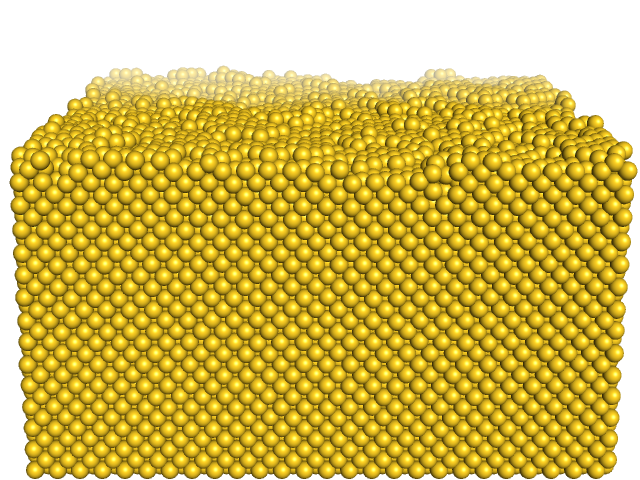
\includegraphics[width=\textwidth]{Au_deposition_flat}
    \subcaption{Glatte, kristalline Schicht ($\sigma_z = \SI{1.2}{\angstrom}$)}
    \label{fig:golddepositions-d}
  \end{subfigure}
  \hfill
  \begin{subfigure}[t]{\subfigwidth}
    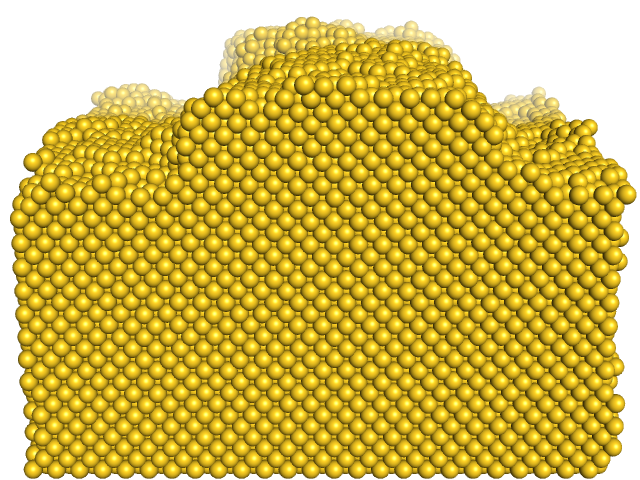
\includegraphics[width=\textwidth]{Au_deposition_step30}
    \subcaption{Fortsetzung der Stufe ($\sigma_z = \SI{6.4}{\angstrom}$)}
    \label{fig:golddepositions-e}
  \end{subfigure}
  \hfill
  \begin{subfigure}[t]{\subfigwidth}
    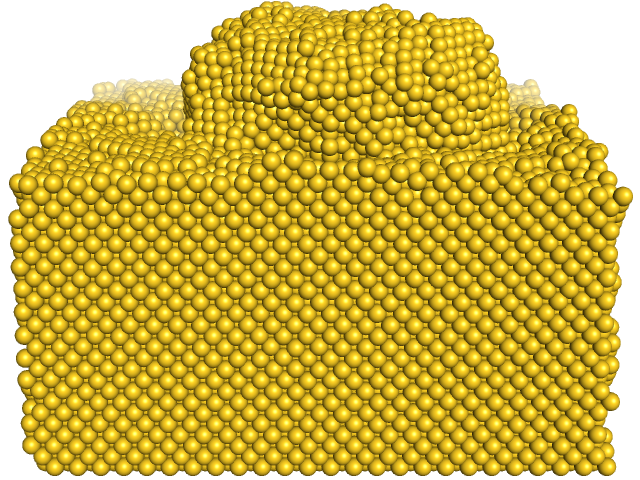
\includegraphics[width=\textwidth]{Au_deposition_tip60}
    \subcaption{Fortsetzung der Spitze ($\sigma_z = \SI{8.0}{\angstrom}$)}
    \label{fig:golddepositions-f}
  \end{subfigure}
  \caption[Gold-Abscheidung auf strukturierten Substraten]{
    Goldschicht nach 50 Abscheidungsschritten (\SI{47}{\angstrom}) auf verschiedenen Substraten
  }
  \label{fig:golddepositions}
\end{figure}

\begin{figure}
  \captionsetup[subfigure]{singlelinecheck=false}
  \def\subfigwidth{0.49\textwidth}

  \begin{subfigure}[t]{\subfigwidth}
    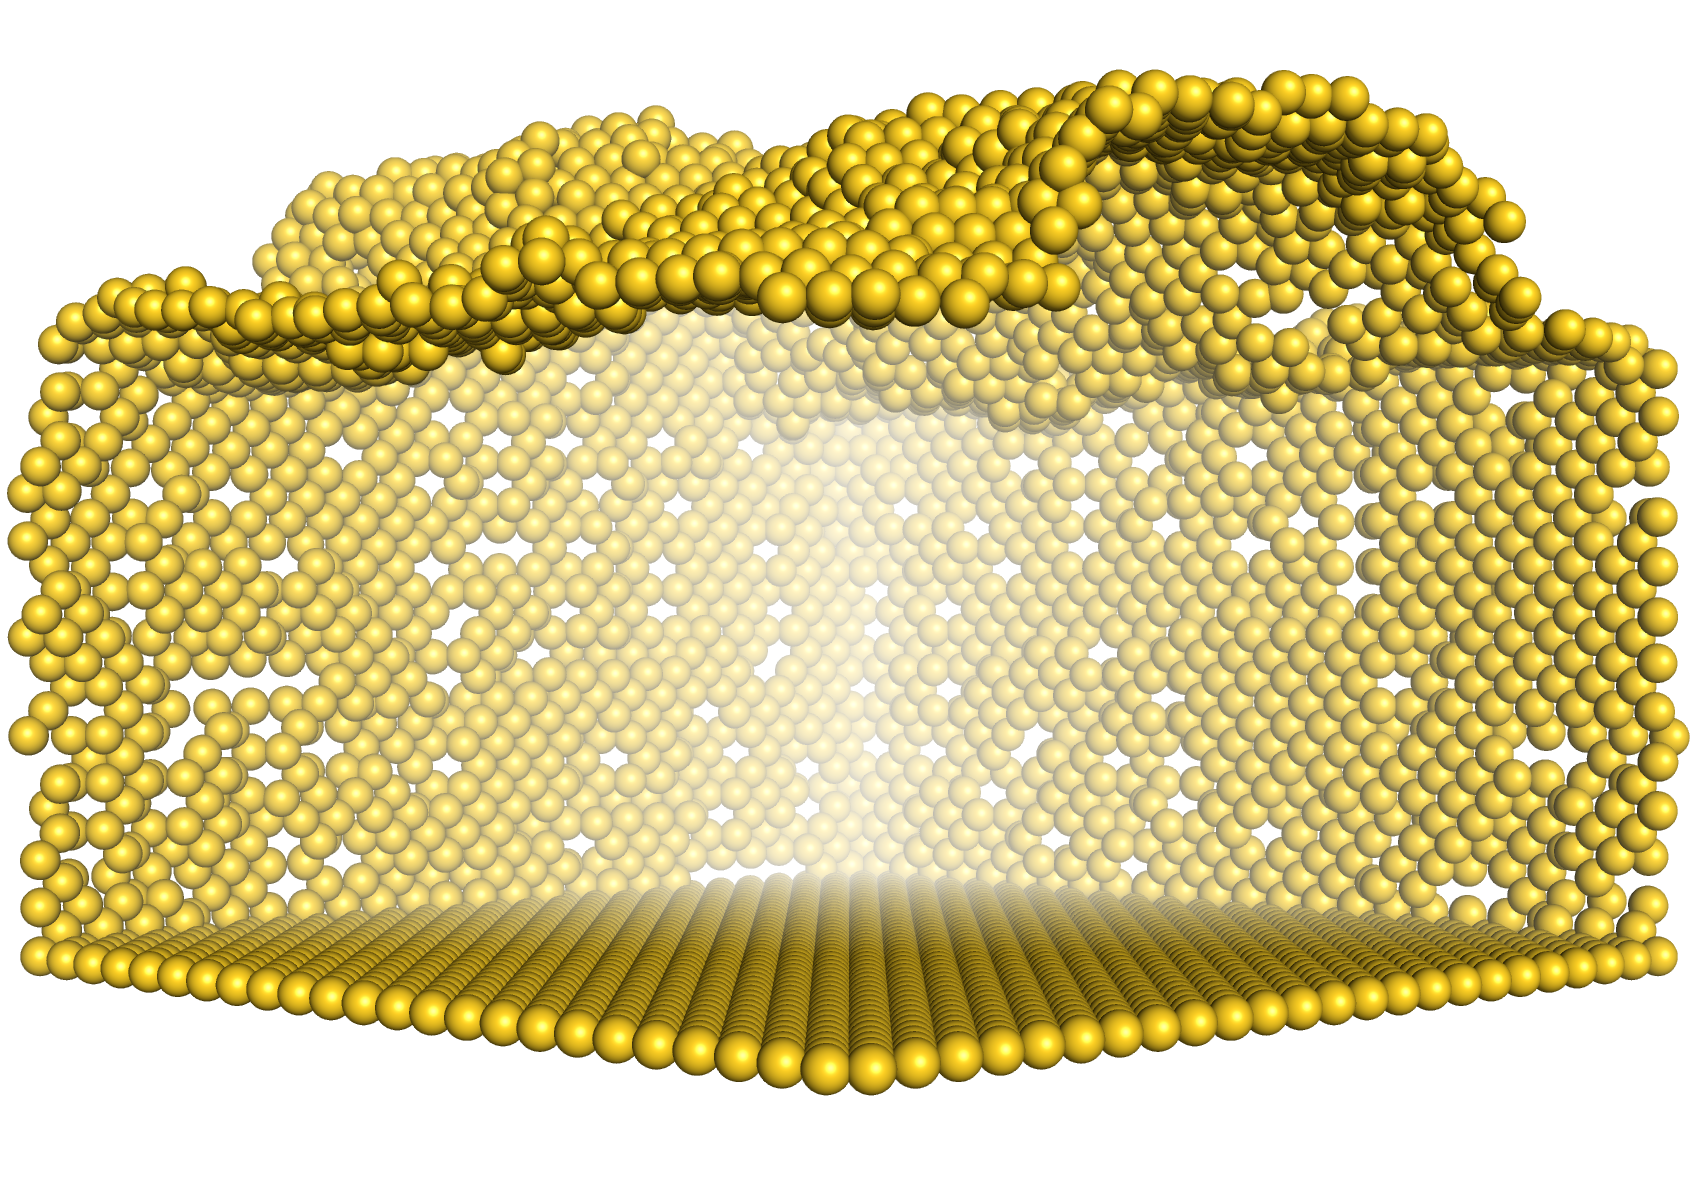
\includegraphics[width=\textwidth]{gold_step30_pockets}
    \subcaption{\SI{30}{\degree}-Stufe: Keine Poren oder Einschlüsse}
    \label{fig:goldpockets-a}
  \end{subfigure}
  \hfill
  \begin{subfigure}[t]{\subfigwidth}
    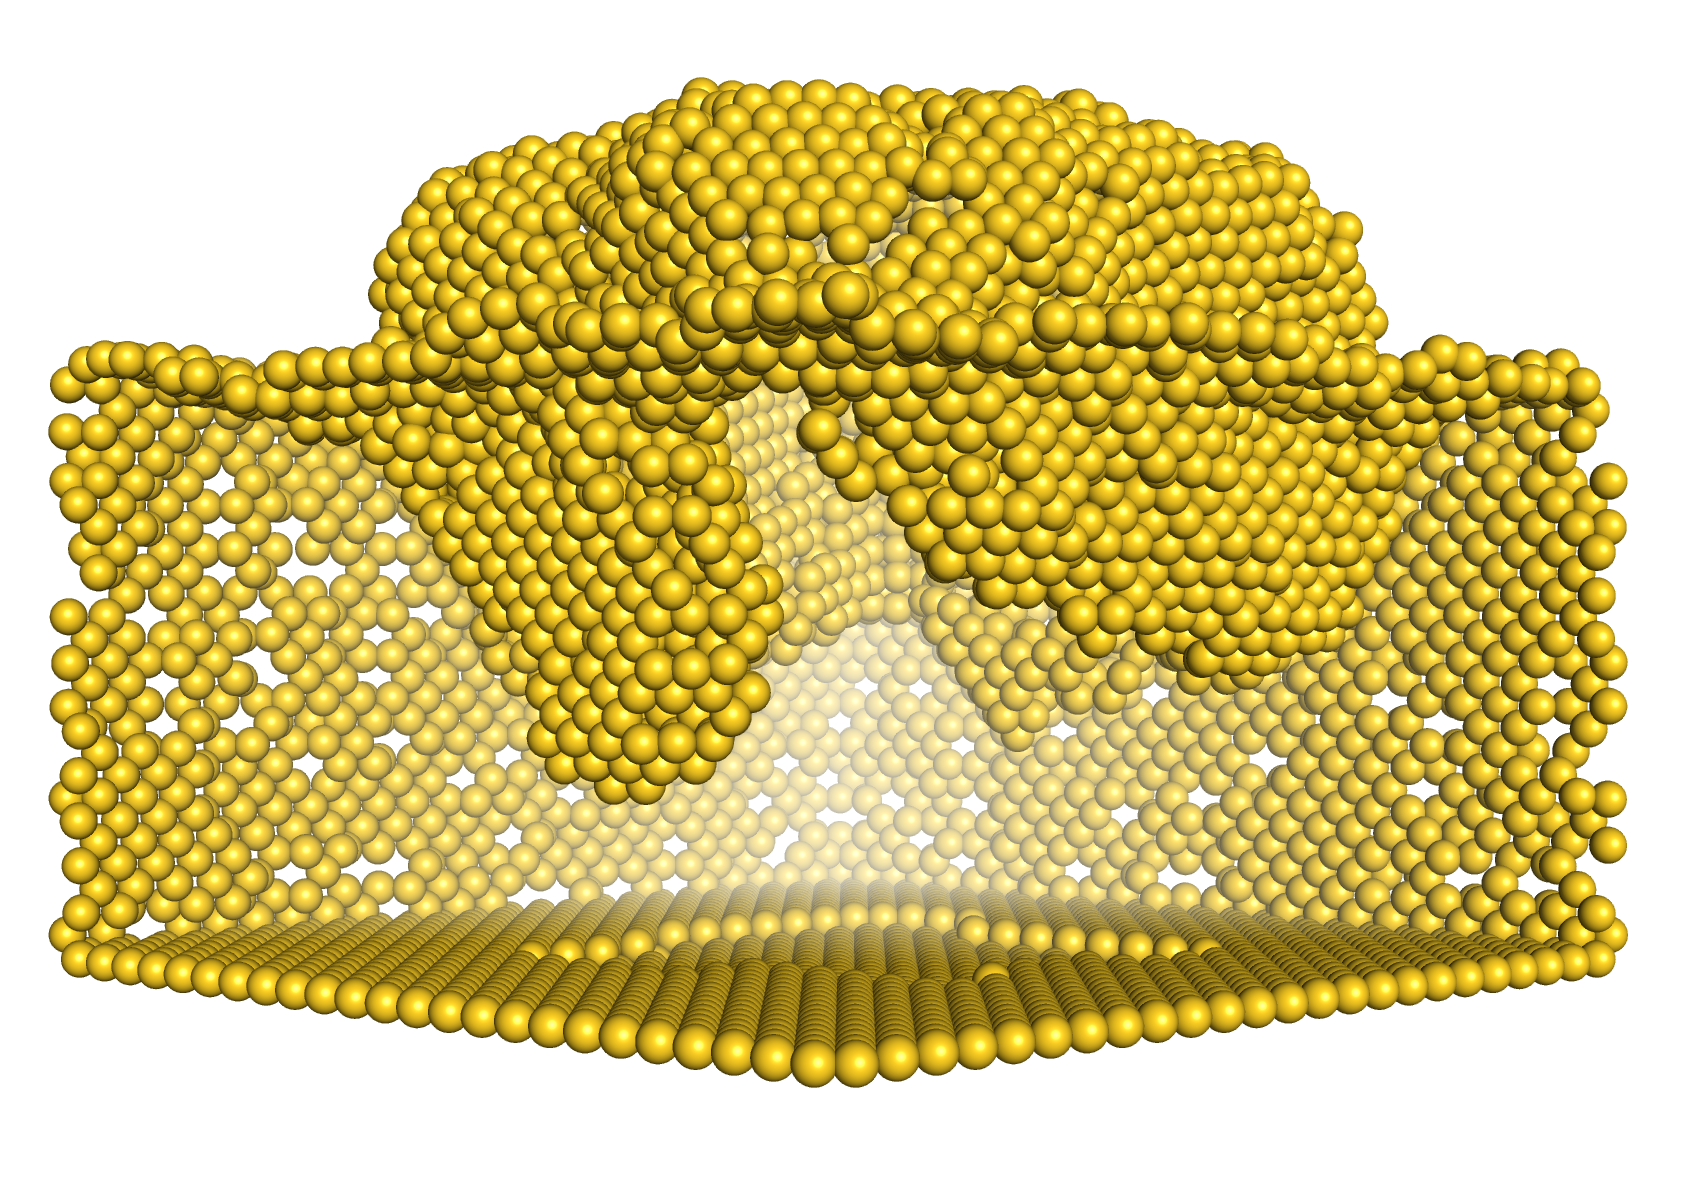
\includegraphics[width=\textwidth]{gold_tip90_pockets}
    \subcaption{Porenbildung an der Basis der \SI{90}{\degree}-Spitze}
    \label{fig:goldpockets-b}
  \end{subfigure}

  \caption[Porenbildung bei Gold-Strukturen]{Porenbildung bei Gold-Strukturen nach 40 Abscheidungsschritten (ca. \num{22000} PVD-Ereignisse $\hat{=}$ \SI{38}{\angstrom}).
  }
  \label{fig:goldpockets}
\end{figure}

Wie man den Alpha-Formen der simulierten Strukturen (Abbildung \ref{fig:goldpockets-a}) entnehmen kann, beinhaltet das abgeschiedene Gold bei geringen Neigungswinkeln keine Kristalldefekte, Poren oder Einschlüsse.
Bei Abscheidungen auf Substrate hoher Neigungswinkel (>\SI{60}{\degree}) bilden sich Poren mit größerer Ausdehnung (>\SI{20}{\angstrom}).
Durch Bildung von Überhängen an den Stufen werden die Poren zu Hohlräumen abgeschlossen, die nicht durch Relaxierung geschlossen werden.
Dies zeigt sich auch in den Oberflächenrauheiten der untersuchten Strukturen (Abbildung \ref{fig:goldroughness}).

\clearpage
\subsection{Vergleich mit gesputterten Schichten}

AFM-Untersuchungen gesputterter Goldschichten zeigen polykristallines Wachstum mit Rauheiten im Bereich von \SI{1.1}{\nano\meter} (etwa drei fcc-Kristallschichten)\cite{svorcik_annealing_2011}.
Dabei wird die Oberflächenrauheit von der Bildung von Nanopartikeln dominiert, deren Schmelztemperaturen mit der Größe der Partikel zunehmen\cite{liu_melting_2001}.
Kleinere Goldpartikeln verschmelzen oberhalb ihrer spezifischen Schmelztemperatur zu größeren Partikeln, wodurch die Rauheit der Goldoberfläche mit höheren Substrat- oder Annealing-Temperaturen zunimmt.
Bei \todo{Vergleich womit?}vergleichsweise niedrigen Temperaturen, wie sie bei Sputtering vorhanden sind, werden durch Unterbindung der Verschmelzung kleiner Goldpartikel geringere Rauheiten erreicht, die mit längerer Sputterdauer weiter abnehmen\cite{svorcik_annealing_2011}.

In Parsivald-Simulationen ist dieser Trend bisher nur selten zu beobachten, wie etwa bei der \SI{45}{\degree}-Spitze, deren Rauheit gegen Ende der Simulation langsam abnimmt.
Die Systeme wachsen in monokristallinen Schichten entlang der Kristallebenen, jedoch zeigen Abscheidungssimulationen auf einigen strukturierten Substraten zusätzliche Porenbildung an Überhängen, die in der aktuellen Oberflächensuche begründet sind.
So wird die Oberfläche und damit mögliche Ereignisorte parallel zur Z-Achse gesucht, anstatt die Alpha-Form über eine Delaunay-Triangulation der Atompositionen zu ermitteln, wie es zur bereits Auswertung der simulierten Strukturen durchgeführt wird.
Somit werden höher gelegene Ereignisorte in der direkten Nachbarschaft bevorzugt, was sich in der Verstärkung von Überhängen bei strukturierten Substraten mit hohen Neigungswinkeln zeigt (Abbildung \ref{fig:goldpockets-b}).
Als Lösung bieten sich die eben genannten Alpha-Formen an, welche jedoch erst für das Parsivald-Modell optimiert werden müssen (Abschnitt \ref{datadelaunay}).

Bei der Analyse der simulierten Strukturen wurde bei Abscheidungen auf glatten Substraten eine Rauheit von \SI{0.12}{\nano\meter} ermittelt, welche nur ca. \SI{10}{\percent} der experimentellen Werte beziehungsweise einer Lage von Goldatomen entspricht.
Strukturierte Substrate zeigen hier höhere Rauheiten, die zwar den experimentell bestimmten Rauheiten entsprechen (Abbildung \ref{fig:goldroughness}), aber ebenfalls keine Nanopartikel enthalten, sondern aus monokristallinen Schichten bestehen.
Daran lässt sich erkennen, dass die verwendeten \todo{word}MD-Simulation-Boxen zu klein und die Relaxationszeiten zu kurz sind, um die Bildung von Nanopartikeln darstellen zu können.
Zusätzlich verhindern kleine MD-Boxen in Verbindung mit monokristallinen Substraten die Ausbildung polykristalliner Strukturen, was sich im Wachstum monokristalliner Schichten äußert.
Derartige Finite-Size-Effekte sind Molekulardynamik-Simulationen inhärent, werden jedoch durch Parsivald für einige Systeme zusätzlich verstärkt.
Bei Abscheidung amorpher Schichten, wie für CVD- und ALD-Prozesse üblich, konnte dieser Effekt bisher nicht beobachtet werden (Abschnitt \ref{siliconpvd}).

\begin{figure}
  \captionsetup[subfigure]{singlelinecheck=false}
  \def\subfigwidth{0.49\textwidth}

  \begin{subfigure}[t]{\subfigwidth}
    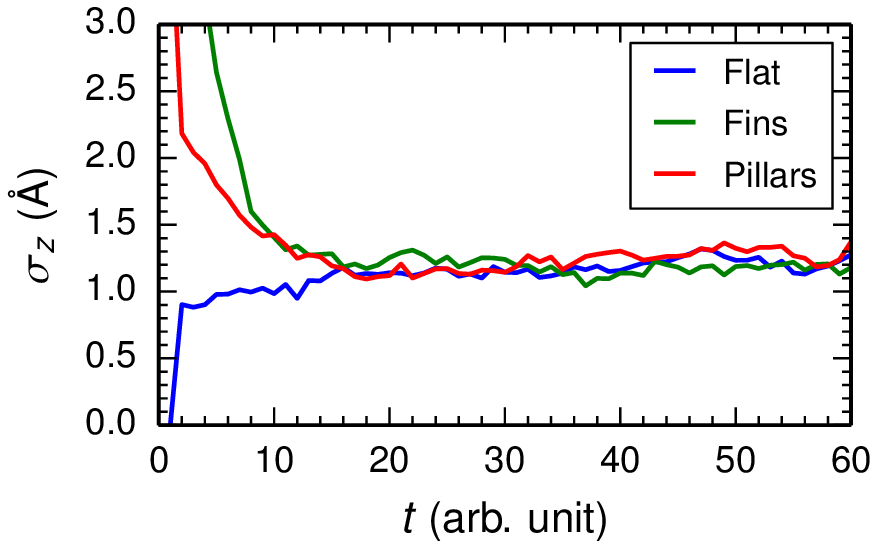
\includegraphics[width=\textwidth]{gold_goodroughness}
    \subcaption{Zeitverlauf der Rauheit von glatten (Flat) und fein strukturierten Oberflächen (Fins, Pillars: \SI{10}{\angstrom} breite Erhebungen)}
    \label{fig:goldroughness-a}
  \end{subfigure}
  \hfill
  \begin{subfigure}[t]{\subfigwidth}
    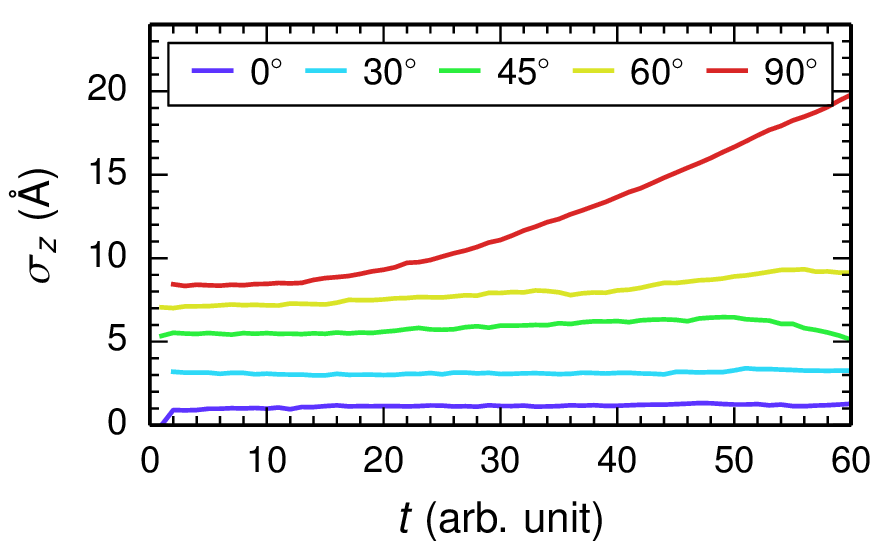
\includegraphics[width=\textwidth]{gold_tiproughness}
    \subcaption{Zeitverlauf der Rauheit von \SI{50}{\angstrom} breiten Spitzen variabler Steigung.
      Oberflächenrauheiten werden nicht verringert
    }
    \label{fig:goldroughness-b}
  \end{subfigure}

  \caption[Oberflächenrauheit von Gold]{Oberflächenrauheit von Gold.
    Im idealen Fall konvergiert die Rauheit gegen einen konstanten Wert von \SI{1.2}{\angstrom}
  }
  \label{fig:goldroughness}

\end{figure}

\subsection{Skalierbarkeit mit der Simulationsgröße}

Die Größe der simulierten Strukturen, wie sie beispielsweise für Beschichtungen kompletter \todo{Nanodevice}Nano-Bauelemente von Interesse sind, ist bei jeder Simulationsmethode durch verschiedene Einflüsse wie Speicherbedarf und Laufzeit limitiert.
Allgemein lässt sich sagen, dass präzisere Methoden nur auf kleineren Systemen und kürzeren Zeitskalen funktionieren (Abbildung \ref{fig:methodscales}).
Atomistische Methoden, insbesondere die Molekulardynamik, sind von theoretischer Seite durch die Notwendigkeit der paarweisen Interaktionen und von technischer Seite durch Speicher- und Netzwerkbandbreite begrenzt.
Somit sind Systeme mit mehr als \num{100000} Atomen nur mit hohem Aufwand über viele Zeitschritte hinweg berechenbar.
Die in Abschnitt \ref{datastructures} vorgestellten Überlegungen zur Optimierung, in Kombination mit dem Parallelisierungsansatz des Parsivald-Modelles aus Abschnitt \ref{parsivald}, sollen hier einem praktischen Test unterzogen werden.

Dazu werden verschiedene quadratische Substrate mit Breiten von \SI{100}{\angstrom}, \SI{200}{\angstrom}, \SI{500}{\angstrom}, \SI{1000}{\angstrom} und \SI{10000}{\angstrom} und \SI{20000}{\angstrom} auf Speicherbedarf, Laufzeit, Anzahl der Atome und Ereignisse, Zahl gleichzeitig aktiver Worker und Bedeckungsgrad der Oberfläche mit aktiven Ereignissen untersucht (Tabelle \ref{tab:goldscalability}).

\begin{table}\begin{threeparttable}

    \caption[asd]{Untersuchungen zur Skalierbarkeit des Systemes}
    \label{tab:goldscalability}

    \begin{tabularx}{\textwidth}{|Xrrrrrrr|}
      \hline
      \textbf{Größe}\tnote{2}  &  \textbf{Wachst.}     &  \textbf{Atome}  &  \textbf{Ereignisse}  &  \textbf{Worker}\tnote{a}  ~            &  \textbf{Bed.}\tnote{e}  &  \textbf{Laufzeit}  &  \textbf{RAM}\tnote{f}  \\
      \hline
      \SI{106}{\angstrom}      &  \SI{70}{\angstrom}   &  \num{59549}     &  \num{46030}          &  \num{1.8}\tnote{b}        (\num{4})    &  \SI{21.9}{\percent}     &  \SI{32.2}{\hour}   &  \SI{254}{\mebi\byte}   \\
      \SI{204}{\angstrom}      &  \SI{42}{\angstrom}   &  \num{152374}    &  \num{102374}         &  \num{14.5}\tnote{b}       (\num{18})   &  \SI{47.7}{\percent}     &  \SI{25.5}{\hour}   &  ~                      \\
      \SI{204}{\angstrom}      &  \SI{42}{\angstrom}   &  \num{152374}    &  \num{102374}         &  \num{14.5}\tnote{b}       (\num{18})   &  \SI{47.7}{\percent}     &  \SI{25.5}{\hour}   &  \SI{257}{\mebi\byte}   \\
      \SI{500}{\angstrom}      &  \SI{93}{\angstrom}   &  \num{1708600}   &  \num{1401081}        &  \num{24.8}                (\num{50})   &  \SI{13.6}{\percent}     &  \SI{73.6}{\hour}   &  \SI{282}{\mebi\byte}   \\
      \SI{1000}{\angstrom}     &  \SI{5.4}{\angstrom}  &  \num{1591908}   &  \num{381588}         &  \num{44.8}                (\num{46})   &  \SI{6.1}{\percent}      &  \SI{1.5}{\hour}    &  \SI{368}{\mebi\byte}   \\
      \SI{1000}{\angstrom}     &  ~                    &  \num{6733948}   &  \num{5539942}        &  \num{75.4}                (\num{149})  &  \SI{10.3}{\percent}     &  \SI{97.5}{\hour}   &  ~                      \\
      \SI{1}{\micro\meter}     &  \SI{1.3}{\angstrom}  &  \num{1.3e8}     &  \num{8186990}        &  \num{25.4}\tnote{c}       (\num{46})   &  \SI{0.03}{\percent}     &  \SI{117.5}{\hour}  &  \SI{11.5}{\gibi\byte}  \\
      \SI{2}{\micro\meter}     &  \SI{0.4}{\angstrom}  &  \num{4.9e8}     &  \num{10356031}       &  \num{26.3}\tnote{c}       (\num{46})   &  \SI{0.009}{\percent}    &  \SI{117.5}{\hour}  &  ~                      \\
      \SI{2}{\micro\meter}     &  \SI{1.0}{\angstrom}  &  \num{5.1e8}     &  \num{25855695}       &  \num{189}\tnote{d}        (\num{245})  &  \SI{0.06}{\percent}     &  \SI{186.8}{\hour}  &  \SI{45.4}{\gibi\byte}  \\
      \SI{4}{\micro\meter}     &  ~                    &  \num{1.9e9}     &  ~                    &  ~                         ~            &  ~                       &  ~                  &  \SI{182}{\gibi\byte}   \\
      \hline
    \end{tabularx}

    \begin{tablenotes}
    \item[2] Breite der quadratischen Oberfläche
    \item[a] Mittelwert und Maximum der zeitgleich bearbeiteten Ereignisse
    \item[b] Maximale Ereignisdichte erreicht.
      Restliche Worker sind im Wartezustand.
    \item[c] Inzwischen behobener Fehler im Host-Code hat Workerneustart verhindert
    \item[d] Maximale Bandbreite des Hosts erreicht.
      Längere MD-Simulationen erlauben mehr Worker.
    \item[e] Bedeckung: Anteil der von laufenden Ereignissen abgedeckten Oberfläche
    \item[f] Vom Hostprozess verbrauchten
    \end{tablenotes}

\end{threeparttable}\end{table}

Mit \SI{94}{\byte} pro Atom, zusätzlich zum konstanten Programmspeicher von \SI{253}{\mebi\byte}, können auch extreme Simulationsräume mit 2 Milliarden Atomen auf einer Oberfläche von \SI{4x4}{\micro\meter} vom Arbeitsspeicher moderner Hochleistungsrechner verwaltet werden können.

Anders sieht es bei der notwendigen Rechenleistung aus:
Während kleine Simulationsräume (\SI{<200}{\angstrom}) nicht wesentlich von der parallelen Rechenleistung profitieren können, scheitern größere Prozesse am Mangel daran:
Im zweiten Test mit einer \SI{2x2}{\micro\meter} großen Struktur wurde die Grenze der Bandbreite des Hostprozesses erreicht:
Die Tests haben gezeigt, dass dieser \num{38.4} Ereignisse pro Sekunde vorbereiten, starten und auswerten kann.
Mit \SI{4.86}{\second} Laufzeit pro Gold-PVD-Ereignis kann der Hostprozess aber nur 189 parallele Worker dauerhaft mit Ereignissen versorgen.
Die eigentliche Beschränkung liegt folglich in der genutzten Potentialart:
Kompliziertere und damit langsamere Potentiale, wie die später genutzten ReaxFF-Potentiale, benötigen meist mehr als \SI{30}{\second} für ein Ereignis, in extremen Fällen sogar \SI{5}{\minute}.
Somit erlauben sie theoretisch \num{1152} beziehungsweise \num{11520} parallele Worker und übersteigen damit die Möglichkeit dessen, was einem einzelnen Nutzer an einem Hochleistungsrechencluster zur Verfügung steht.
Leider erhöht sich damit auch die insgesamt benötigte Rechenzeit linear.

Die verbleibende Einschränkung wird somit von den verfügbaren Rechenkernen gebildet.
In Simulationen mit Substratgrößen auf der Mikrometer-Skala wurden nur kleine Teile der Oberfläche (\SI{<0.1}{\percent}) zeitgleich von Ereignissen simuliert.
Bei Oberflächen von \SI{2x2}{\micro\meter} Größe sind in dichtester Packung der MD-Boxen mit je \SI{37x37}{\angstrom} Größe maximal \num{291600} parallele Ereignisse möglich.
Tatsächlich werden aufgrund der Überdeckung der Ereignisse durch die zufällige Wahl der Reaktionsorte häufig \SI{<40}{\percent} davon zeitgleich simuliert.
Dennoch liegt die Zahl der verfügbaren Prozessorkerne um Größenordnungen unterhalb des optimalen Wertes, was sich in langen Simulationslaufzeiten äußert (\SI{186.8}{\hour} für \SI{1.0}{\angstrom}).

Zusammenfassend lässt sich sagen, dass Systeme mit einer Größe zwischen \SI{50x50}{\nano\meter} und \SI{300x300}{\nano\meter} mit modernen Computerclustern effizient berechenbar sind, wo hingegen kleinere Systeme nicht signifikant von der Effizienzsteigerung profitieren können und für größere Systeme die notwendige Rechenleistung unerreichbar bleibt.


  \clearpage
  \section{Kupfer-PVD}
\label{copperpvd}

Ein zweites PVD-System stellt Kupfer dar, wofür eine Vielzahl an unterschiedlichen Parametrisierungen vorliegen (Tabelle \ref{tab:copperpots}).
Es stellt sich die Aufgabe, eine passende Parametrisierung darunter zu suchen und zu entscheiden, inwiefern eine Vorauswahl anhand weniger Parameter \todo{chword} sinnvoll ist.
Kupfer bildet ebenfalls fcc-Kristalle, 

\begin{table}[hbtp]
  \caption[EAM-Parametrisierungen für Kupfersysteme]{EAM-Parametrisierungen für Kupfersysteme.}
  \label{tab:copperpots}
  \rowcolors{0}{white}{lightgray}
  \begin{tabularx}{\textwidth}{|lXc|}
    \hline
    \textbf{Bezeichnung} & \textbf{Anwendung \& Kommentare} & \textbf{Ref.} \\
    \hline
    CuAg.eam.alloy & Strukturelle und thermische Eigenschaften von \ce{Cu-Al} & \cite{williams_embedded-atom_2006} \\
    cu\_ag\_ymwu.eam.alloy & Mono-, Di-, Trimere und Inseln von \ce{Cu} auf \ce{Ag} & \cite{wu_cu/ag_2009} \\
    Cu\_smf7.eam & Oberflächen von \ce{Ni-Cu}-Legierungen bei \SI{800}{\kelvin} & \cite{foiles_calculation_1985} \\
    Cu\_u3.eam & Oberflächen und Bulks verschiedener Legierungen & \cite{foiles_embedded-atom-method_1986} \\
    Cu\_u6.eam & Aktivierungsenergie für Eigendiffusionen & \cite{adams_self-diffusion_1989} \\
    Cu-Zr\_2.eam.fs & Flüssige und amorphe \ce{Cu-Zr}-Legierungen & \cite{mendelev_development_2009} \\
    Cu-Zr.eam.fs & Flüssige und amorphe \ce{Cu-Zr}-Legierungen & \cite{mendelev_using_2007} \\
    Mendelev\_Cu2\_2012.eam.fs & Unterkühlte \ce{Al-Cu}-Schmelzen. Basiert auf \cite{mendelev_analysis_2008} & \cite{_interatomic_2014} \\
    \hline
  \end{tabularx}
  
\end{table}

\subsection{Voruntersuchungen}

Bei den Voruntersuchungen der strukturellen Eigenschaften konnten einige Parametersätze von LAMMPS nicht akzeptiert werden oder haben sich mit kryptischen Fehlern auf negative Speicherallokierungen aufgehangen.
Die Ergebnisse der drei verbliebenen Potentiale sind jedoch in guter Übereinstimmung mit Literaturwerten (Tabelle \ref{tab:copperpreresults}).
\todo{Dichte}Der Schmelzpunkt wurde jedoch nicht zuverlässig simuliert (Abbildung \ref{fig:copperthermo}).

\begin{table}[hbtp]
  %% \rowcolors{0}{white}{lightgray} 
  \caption[Eigenschaften von Gold]{Vergleich der Eigenschaften von Gold mit experimentellen und Literaturdaten als Voruntersuchung des PVD-Prozesses\todo[inline]{ref}}
  \label{tab:goldpreresults}
  \begin{tabularx}{\textwidth}{|lXXXX|}
    \hline
    \textbf{unters. Größe} & \textbf{Experiment} & \textbf{Cu\_smf7.eam} & \textbf{Cu\_u3.eam} & \textbf{Cu\_u6.eam} \\
    \hline
    Bindungslänge  &  \SI{2.556}{\angstrom} & \SI{2.558}{\angstrom} & \SI{2.558}{\angstrom} & \SI{2.558}{\angstrom} \\
    Koordination   &  \SI{12.00}{} & \SI{12.00}{} & \SI{12.00}{} & \SI{12.00}{} \\
    Dichte         & \SI{8.92}{\gram\per\cubic\centi\meter} & \SI{8.908}{\gram\per\cubic\centi\meter} & \SI{8.915}{\gram\per\cubic\centi\meter} & \SI{8.910}{\gram\per\cubic\centi\meter} \\
    \hline
  \end{tabularx}
\end{table}

\todo[inline]{Oberflächenvalidierung?}

\begin{figure}[tbp]
  \centering
  \captionsetup[subfigure]{singlelinecheck=false}
  \def\subfigwidth{7cm}
  \begin{subfigure}[t]{\subfigwidth}
    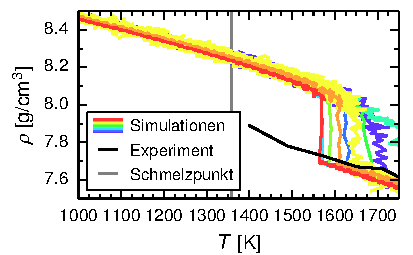
\includegraphics[width=\textwidth]{Cu_u6_meltingpoint}
    \subcaption{Phasenübergang mit Cu\_u6.eam bei unterschiedlichen $t_\text{relax}$}
  \end{subfigure}
  \hfill
  \begin{subfigure}[t]{\subfigwidth}
    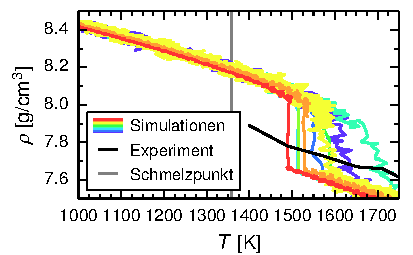
\includegraphics[width=\textwidth]{Cu_smf7_meltingpoint}
    \subcaption{Phasenübergang mit Cu\_smf7.eam bei unterschiedlichen $t_\text{relax}$}
  \end{subfigure}
  \caption[Abweichung der Schmelztemperaturen bei Kupfer-MD]{
    Abweichung der Schmelztemperatur mit verschiedenen Parametrisierungen.
    Experimentelle Werte von Brillo et al.\cite{brillo_density_2006}.
  }
  \label{fig:goldthermo}
\end{figure}

\subsection{Prozess-Simulation}

Äquivalent zur Vorgehensweise beim Gold-PVD-Prozess wurde ein Kupfer-PVD-Prozess gestartet
Zur Simulation eines Gold-PVD-Prozesses mit Parsivald wurden die untersuchten Potentialparameter sowie ein Kristallsubstrat eingelesen, ein Abscheidungsmodus mit zufälligen Auftreffpositionen in der xy-Ebene gewählt und Relaxationszeiten und Reaktionsnachbarschaftsgrößen gewählt, die in den vorheringen Tests als hinreichend ermittelt wurden.
Damit ergaben sich Reaktionsräume der Größe \SI{37x37x25}{\angstrom} mit jeweils ca. 1800 Atomen, Relaxationszeiten von \SI{1.4}{\nano\second} in \SI{1400}{} Simulationsschritten und Auftreffgeschwindigkeiten von \SI{4}{\angstrom/\pico\second}, die aus üblichen Sputterbedingungen stammen.\todo{wie berechnet?}
Die \SI{100x100}{\angstrom} breiten Kristalle werden perfekt fortgesetzt, wobei nach 10 Kristallschichten eine Rauheit von einem Atomdurchmesser vorliegt, was Übereinstimmung mit einem diffusionsdominierten Abscheidungsprozess zeigt.

\subsubsection{Strukturierte Substrate}

Als Stabilitätsprüfung wurden auch Abscheidungen auf strukturierten Substraten (Abbildung \ref{fig:coppersubstrate}) mit den gleichbleibenden Prozessbedingungen simuliert.
Es wurden Stufen und Spitzen mit Neigungen von jeweils \SI{15}{\degree}, \SI{20}{\degree}, \SI{30}{\degree}, \SI{45}{\degree}, \SI{60}{\degree} und \SI{90}{\degree} bei oben genannten Prozessbedingungen untersucht.
\todo{vorherige Relaxation?}

\begin{figure}[bt]
  \captionsetup[subfigure]{singlelinecheck=false}
  \def\subfigwidth{0.31\textwidth}
  \begin{subfigure}[t]{\subfigwidth}
    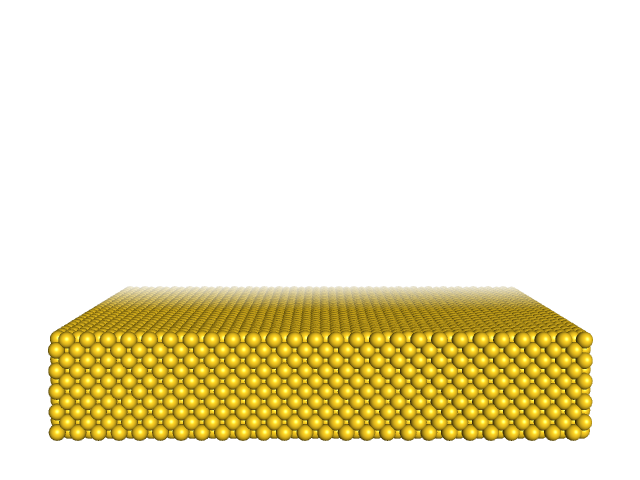
\includegraphics[width=\textwidth]{Au_substrate_flat}
    \subcaption{Glattes Gold-Substrat}
    \label{fig:coppersubstrate-a}
  \end{subfigure}
  \hfill
  \begin{subfigure}[t]{\subfigwidth}
    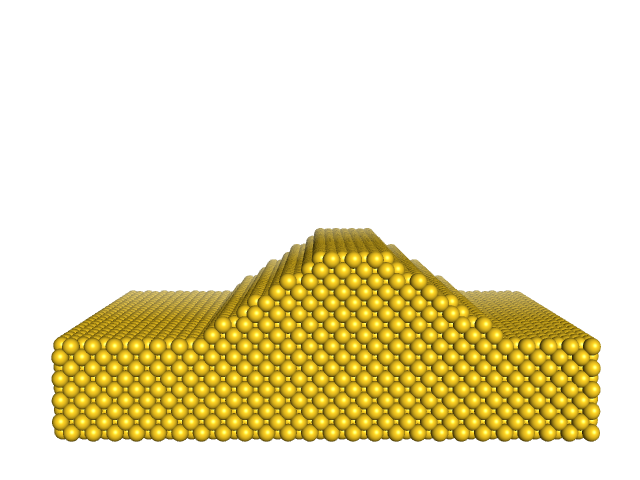
\includegraphics[width=\textwidth]{Au_substrate_step30}
    \subcaption{Gold-Stufe, \SI{30}{\degree}}
    \label{fig:coppersubstrate-b}
  \end{subfigure}
  \hfill
  \begin{subfigure}[t]{\subfigwidth}
    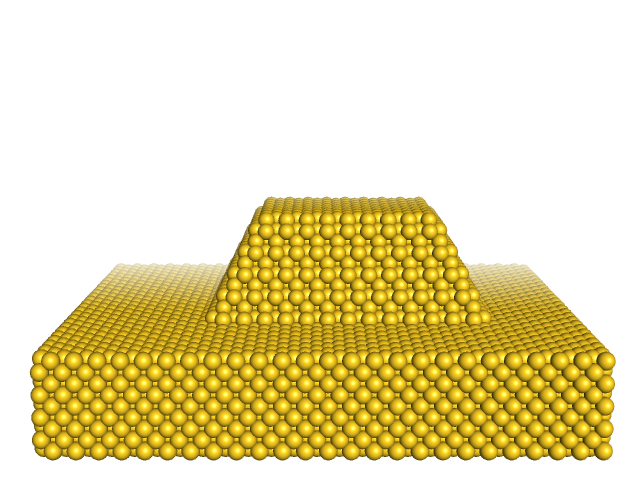
\includegraphics[width=\textwidth]{Au_substrate_tip60}
    \subcaption{Gold-Spitze, \SI{60}{\degree}}
    \label{fig:coppersubstrate-c}
  \end{subfigure}
  \caption[Strukturierte Coppersubstrate]{Coppersubstrate mit unterschiedlicher Struktur und Breite und Tiefe von \SI{100}{\angstrom}.
    Abscheidungen wurden auf glatten Substraten, Stufen und Spitzen vorgenommen.}
  \label{fig:coppersubstrate}
\end{figure}

\begin{figure}[bt]
  \captionsetup[subfigure]{singlelinecheck=false}
  \def\subfigwidth{0.31\textwidth}
  \begin{subfigure}[t]{\subfigwidth}
    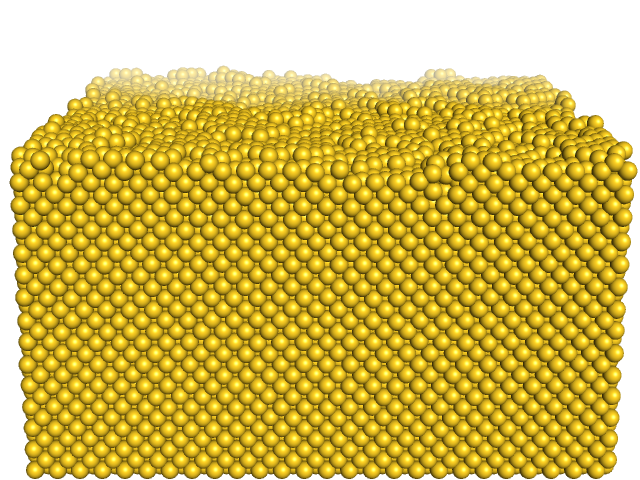
\includegraphics[width=\textwidth]{Au_deposition_flat}
    \subcaption{Abscheidung auf glattem Gold-Substrat}
    \label{fig:copperdepositions-a}
  \end{subfigure}
  \hfill
  \begin{subfigure}[t]{\subfigwidth}
    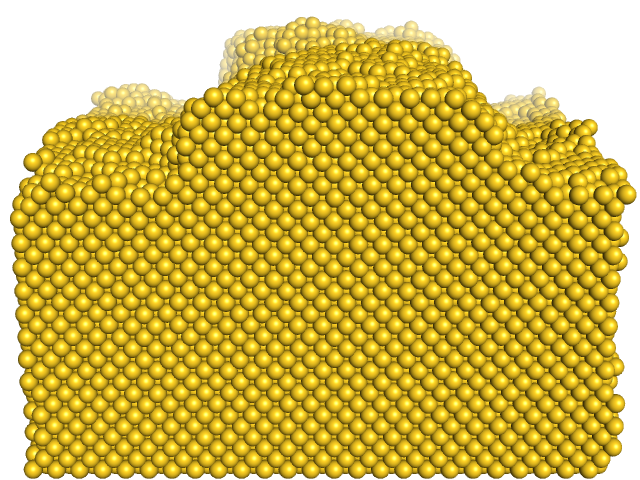
\includegraphics[width=\textwidth]{Au_deposition_step30}
    \subcaption{Abscheidung auf Gold-Stufe, \SI{30}{\degree}}
    \label{fig:copperdepositions-b}
  \end{subfigure}
  \hfill
  \begin{subfigure}[t]{\subfigwidth}
    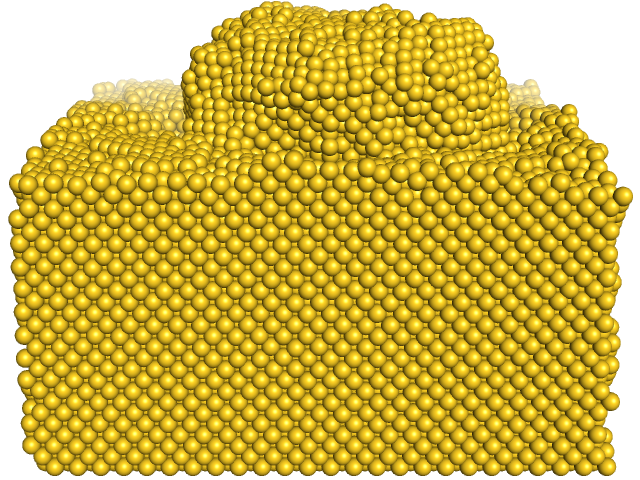
\includegraphics[width=\textwidth]{Au_deposition_tip60}
    \subcaption{Abscheidung auf Gold-Spitze, \SI{60}{\degree}}
    \label{fig:copperdepositions-c}
  \end{subfigure}
  \caption[Abscheidung auf strukturierten Substraten]{
    Ergebnis der Abscheidung.
    Die Substratstruktur bleibt erkennbar, wird aber nach oben verstärkt, ansonsten aber kristallin und glatt fortgesetzt.
  }
  \label{fig:copperdepositions}
\end{figure}

Das Kristallsubstrat wird auch hier fortgesetzt, jedoch verstärken sich Neigungswinkel an Stufen und Spitzen zunehmend.
Nach längeren Laufzeiten entstehen somit Überhänge, die durch Abschluss von unten zu Hohlräumen innerhalb der Struktur führen, welche in der Realität durch thermische Relaxation geschlossen würden.
Dahinter steht einerseits die Notwendigkeit, Gold-Atome bei Ankunft auf der Oberfläche ausreichend diffundieren zu lassen, was beim aktuellen Modell nur innerhalb der Reaktionsraumgrenzen geschieht.

Andererseits liegt ein methodischer Fehler bei Nutzung von Binning-Methoden vor:
Die Oberfläche wird aus algorithmischen Gründen nur entlang der z-Achse bestimmt, woraufhin das neue Atom oberhalb eines Referenzatomes auf der Oberfläche platziert wird.
An Stufen und Kanten werden hierbei höhere Reaktionsorte bevorzugt, an denen das Atom mit \todo{phrasing}statistischer Wahrscheinlichkeit verbleibt.

Einen Lösungsansatz stellt die ausführliche Parametrisierung der Oberfläche dar, beispielsweise per Alpha-Form (siehe Abschnitt \ref{dataalphaform}, über die man die Ereigniswahrscheinlichkeit entsprechend der Einbettungsenergie variierte, angenähert über die Oberflächenkrümmung.

  \clearpage
  \section{Multilagen-PVD}
\label{multilayer}

Mit PVD-Methoden können auch mehrlagige Schichten abgeschieden werden, die im folgenden Kapitel am Beispiel von dünnen Cu/Ni-Multilagen näher untersucht werden sollen.
Das Kupfer-Nickel-System wurde aufgrund ähnlicher Gitterkonstanten gewählt (Ni:~\SI{3.52}{\angstrom}, Cu:~\SI{3.61}{\angstrom}), die kristallines Wachstum ermöglichen und somit Fehlstellen unterbinden.
Durch die Ähnlichkeit zur Kupfer-PVD kann man zudem auf den dort entwickelten Prozessparametern und den untersuchten Potentialparametersätzen aufbauen.

Im Experiment werden mehrlagige Kupfer-Nickel-Schichten per Elektro\-deposition\cite{yang_pulsed_1995} oder durch Sputtern\cite{cammarata_nanoindentation_1990} hergestellt, wobei üblicherweise Lagendicken im Bereich mehrerer Nanometer erzielt werden.
Dieses Vorgehen lässt sich direkt in Parsivald-Simulationen übertragen, in denen zugunsten der Rechenzeit in den folgenden Untersuchungen vergleichsweise dünne Lagen mit einer Dicke von \SI{1}{\nano\meter} abgeschieden wurden.
Anschließend werden diese auf Ähnlichkeit mit LAMMPS-präparierten Multilagen hinsichtlich ihrer Lagendicke und -rauheit untersucht.
Eine Auswertung der relativen Verteilung der Spezies entlang der Abscheidungsrichtung wird ergänzend für verschiedene Relaxationszeiten als Maß der Lagenqualität durchgeführt.
Abscheidungen von Lagen mit einer Dicke von \SI{6}{\nano\meter} wurden ebenfalls mit Parsivald simuliert, doch mangels verfügbarer Rechenzeit für vergleichbare LAMMPS-Simulationen nicht eingehender untersucht.

Wie bei den Gold-PVD-Simulation zuvor müssen für erfolgreiche Simulationen einige Prozessparameter wie Relaxationszeit, Thermostatdämpfung und Substrattemperatur optimiert werden.
Als Zielgrößen für die Optimierung wurden zur Vermeidung von Fehlstellen die Rauheit der Oberfläche und die Qualität der einzelnen Lagen im Vergleich mit ähnlichen Untersuchungen\cite{zhou_atomistic_1998} gewählt.
In diesen Untersuchungen wurde bereits gezeigt, dass die kinetische Energie der einfallenden Atome einen erheblichen Einfluss auf die Qualität der einzelnen Lagen hat, weshalb gleichartige Untersuchungen nur hinsichtlich der Substrattemperatur durchgeführt wurden.

\subsection{Ergebnisse}

Parsivald-Simulationen erzeugen nach korrekter Parametereinstellung monokristallin gewachsene, klar abgegrenzte Atomlagen geringer Rauheit, die sich gut mit den Ergebnissen gleichartiger LAMMPS-Simulationen decken (Abbildung~\ref{fig:multilayerresults}).
RMS-Rauheiten um \SI{1.2}{\angstrom} stellen sich mit beiden Simulationsmethoden bis zur zehnten Lage ein und stimmen somit miteinander und mit den bisherigen Ergebnissen überein (Abbildung~\ref{fig:multilayerplots-a}).

Zuvor war eine Anpassung der Temperaturen und Relaxationszeiten notwendig, die jedoch für LAMMPS und Parsivald gleichermaßen gelten.
Als Richtwert wurde die Qualität der einzelnen Lagen in Form des Anteils der Spezies in Abhängigkeit der Höhe über dem Substrat genutzt (Abbildung~\ref{fig:multilayerplots-b}).
Lagen schlechterer Qualität zeigen eine höhere Durchmischung der Schichten, was wiederum zu einer Senkung der relativen Häufigkeit einer Spezies innerhalb ihrer Schicht führt, wie man für die beiden Verteilungen bei einer Relaxationszeit von \SI{0.2}{\femto\second} pro Ereignis beobachten kann.
Erst bei Verdopplung der Relaxationszeit bilden sich klar abgegrenzte Lagen aus, wie sie in Abbildung~\ref{fig:multilayerresults} dargestellt sind.

In Anhang~\ref{appendix:multilayer} ist eine Auswahl von mehrlagigen Kupfer-Nickel-Schichten dargestellt, die durch Unterrelaxation verursachte strukturelle Fehler aufweisen.
Bei größeren Systemen ist zudem mit Verspannungen aufgrund der unterschiedlichen Bindungslängen Gitterversetzungen und Fehlstellen zu rechnen, die allerdings durch Finite-Size-Effekte unterdrückt sein können.

\begin{figure}
  \captionsetup[subfigure]{singlelinecheck=false}
  \def\subfigwidth{7cm}
  \begin{subfigure}[t]{\subfigwidth}
    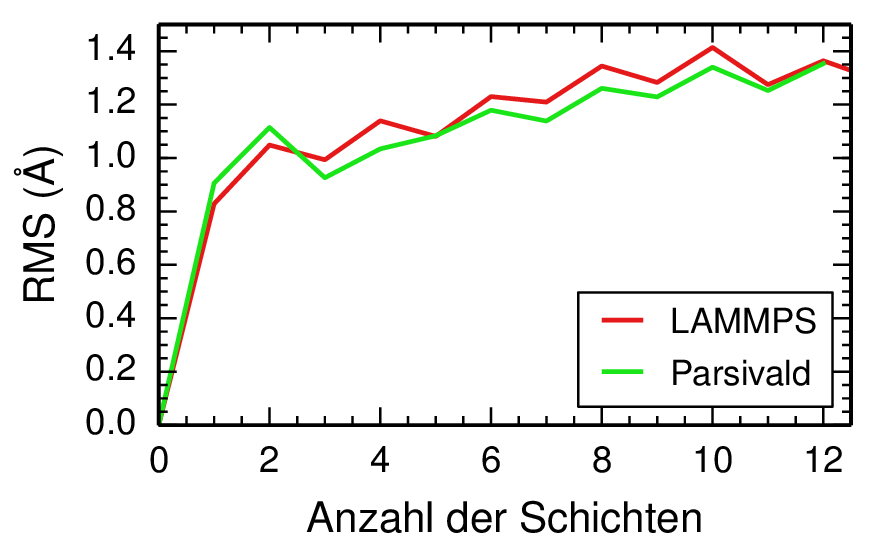
\includegraphics[width=\textwidth]{CuNi_layerroughness_comparison}
    \subcaption{
      Vergleich der Lagen-Rauheit (Abb.~\ref{fig:multilayerresults})
    }
    \label{fig:multilayerplots-a}
  \end{subfigure}
  \hfill
  \begin{subfigure}[t]{\subfigwidth}
    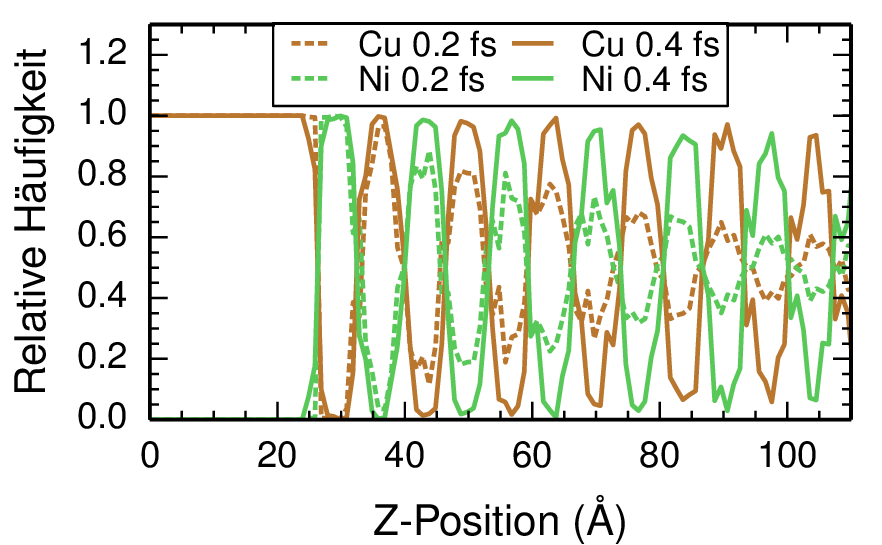
\includegraphics[width=\textwidth]{CuNi_atomdistribution_relax}
    \subcaption{Einfluss von $t_\text{relax}$ auf die Lagen-Qualität}
    \label{fig:multilayerplots-b}
  \end{subfigure}
  \caption[Rauheit und Qualität von Kupfer-Nickel-Multilagen]{
    Rauheit und Qualität von Kupfer-Nickel-Multilagen
  }
  \label{fig:multilayerplots}
\end{figure}

\begin{figure}
  \captionsetup[subfigure]{singlelinecheck=false}
  \def\subfigwidth{7cm}
  \begin{subfigure}[t]{\subfigwidth}
    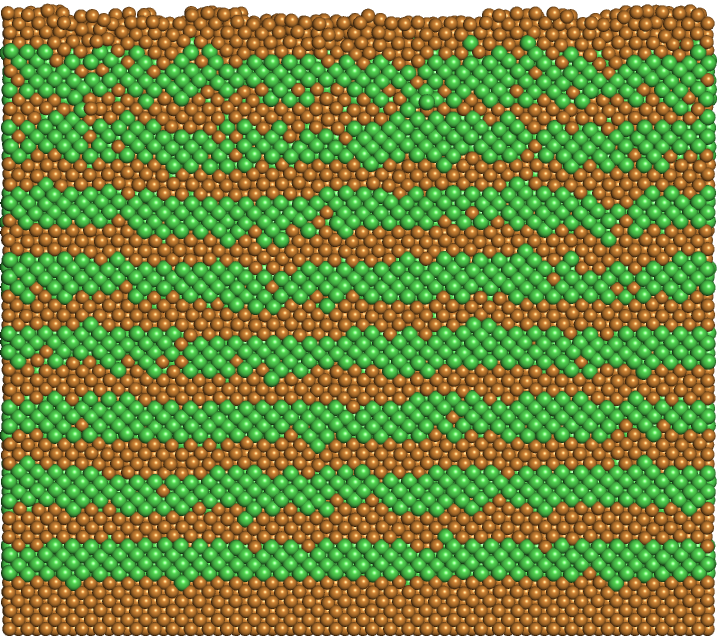
\includegraphics[width=\textwidth]{CuNi_profile_LAMMPS_nice}
    \subcaption{Profil von \ce{CuNi}-Multilagen mit LAMMPS}
  \end{subfigure}
  \hfill
  \begin{subfigure}[t]{\subfigwidth}
    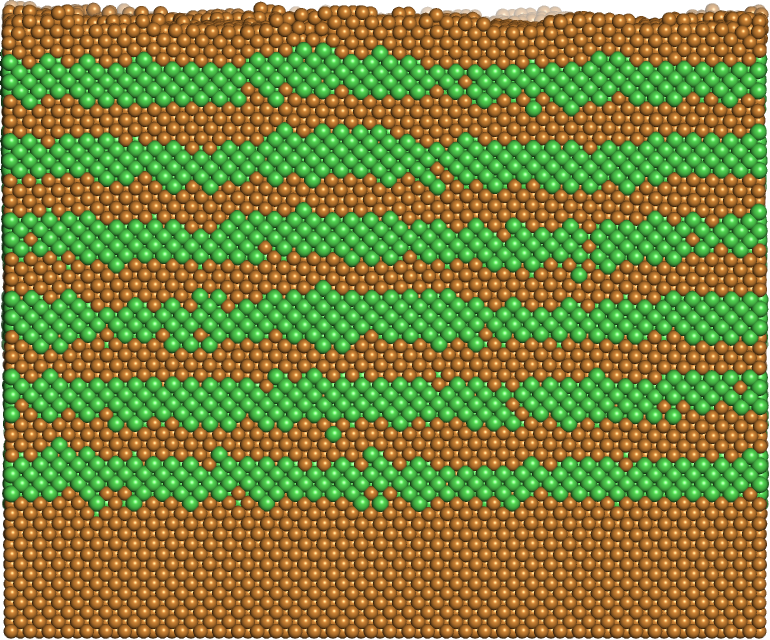
\includegraphics[width=\textwidth]{CuNi_profile_Parsivald}
    \subcaption{Profil von \ce{CuNi}-Multilagen mit Parsivald}
  \end{subfigure}
  \caption{Vergleich von Multilagen-Profilen mit LAMMPS und Parsivald}
  \label{fig:multilayerresults}
\end{figure}

  \clearpage
  \section{Silizium-PVD}
\label{siliconpvd}

Mit Silizium soll ein weiteres PVD-Material untersucht werden, das im Gegensatz zu den bisher untersuchten Metallen, welche ungerichtete Bindungen aufbauen und damit die kristalline Strukturen bevorzugen, auf gerichteten Bindungen beruht.
Deshalb werden reaktive Kraftfelder genutzt, welche auf einer expliziten Beschreibung gerichteter Bindungen über Bindungsordnungen benachbarter Atome basieren.

\subsection{Verfügbare ReaxFF-Parametrisierungen}

Da die ReaxFF-Formulierung erst innerhalb des letzten Jahrzehntes an Popularität gewonnen hat, sind die verfügbaren Potentiale auf sehr spezielle Probleme angepasst und unterstützen meist entweder Bulkmaterialien oder Reaktionen zwischen Molekülen.
Tabelle~\ref{tab:siliconpotentials} listet die im Rahmen der Arbeit untersuchten ReaxFF-Parametrisierungen auf, die in der Literatur gefunden werden konnten.

\begin{table}[hb]
  \caption{Untersuchte ReaxFF-Parametrisierungen für Silizium- und Siliziumoxidsysteme}
  \label{tab:siliconpotentials}
  \oddrowcolors
  \begin{tabularx}{1\textwidth}{|lXc|}
    \hline
    \textbf{Bezeichnung}  & \textbf{Anwendung \& Kommentare}                                                                          & \textbf{Ref.}                     \\
    \hline
    \pot{Al\_Al0\_AlN}    & \ce{Al}, \ce{Al2O3}, \ce{AlN}. Basiert auf einer Si-Parametrisierung                                      & \cite{plimpton_lammps_2014}       \\
    \pot{chenoweth}       & Zersetzung von Polydimethylsiloxane bei hohen Drücken und Temperaturen. Ergänzung von \ce{C-Si}-Bindungen & \cite{chenoweth_simulations_2005} \\
    \pot{kulkarni}        & Reaktion von Sauerstoff mit \ce{OH}-terminierten Siliziumoxid-Oberflächen                                 & \cite{kulkarni_oxygen_2013}       \\
    \pot{lg}              & ``low gradients''. Siehe liu\_nitramines. Fehlerhafte Version aus LAMMPS                                  & \cite{liu_reaxff-lg:_2011}        \\
    \pot{liu\_ettringite} & Verspannung von Ettringit (\ce{Ca6[Al(OH)6]2(SO4)3 26H2O}). Basiert auf Si-Parametrisierung               & \cite{liu_development_2012}       \\
    \pot{liu\_nitramines} & Dichtebestimmung von Nitramin-Molekülen bei hohen Drücken. Dichte erhöht durch Van-der-Waals-Korrekturen  & \cite{liu_reaxff-lg:_2011}        \\
    \pot{narayanan}       & Präparation mit \ce{Li-Al}-Silikaten. Für Phasenübergänge von Eukryptit-Kristallen (\ce{LiAl[SiO4]})      & \cite{narayanan_reactive_2012}    \\
    \pot{newsome}         & Oxidation von \ce{SiC}-Oberflächen mit \ce{O2} und \ce{H2O} bei \SIrange{500}{5000}{\kelvin}              & \cite{newsome_oxidation_2012}     \\
    \pot{nielson}         & Reaktionskinetik an Metallkatalysatoren bei hohen Temperaturen                                            & \cite{nielson_development_2005}   \\
    \pot{zhang}           & Zersetzung energetischer Moleküle (Nitramin-Explosionen)                                                  & \cite{zhang_carbon_2009}          \\
    \hline
  \end{tabularx}
\end{table}

\subsection{Voruntersuchungen}

In Ergänzung zu den bisherigen Voruntersuchungen, welche sich entsprechend der erwarteten Strukturen der abgeschiedenen Schichten auf die Beschreibung kristalliner Strukturen beschränkten, werden für die Silizium-Parametrisierungen auch die Eigenschaften amorpher Strukturen untersucht.
Die verwendeten Methoden wurden bereits in Abschnitt~\ref{mdmethods} vorgestellt.
Diese zusätzlichen Untersuchungen haben umfassendere Aussagen über die Anwendbarkeit der Parametrisierungen für vollständige Abscheidungssimulationen zum Ziel.
Die Ergebnisse dieser Betrachtungen sind in Tabelle~\ref{tab:siliconpreresults} zusammen gefasst und werden im Weiteren kurz diskutiert.

\begin{table}[th]
  \begin{threeparttable}
    \caption[Zusammenfassung der Voruntersuchungen für Silizium-Systeme]{
      Zusammenfassung der Voruntersuchungen für Silizium-Systeme.
      Siehe Anhang~\ref{appendix:silicon}
    }
    \label{tab:siliconpreresults}

    \oddrowcolors
    \begin{tabularx}{\textwidth}{|lCCCCCCC|}
      \hline
      \textbf{Bezeichnung}    & LMP\tnote{a} & c-\ce{Si} & c-\ce{SiO2} & a-\ce{Si} & \ce{SiH4} & \ce{+O2} & PVD\tnote{b} \\
      \hline                % & LAMMPS       & c-Si      & c-SiO2      & a-Si      & Silane    & +O2      & PVD          \\
      \pot{Al\_Al0\_AlN}      & \cmark       & ~         & (\cmark)    & \cmark    & \cmark    & ~        & \cmark       \\
      \pot{chenoweth}         & ~            & ~         & ~           & ~         & ~         & ~        & ~            \\
      \pot{kulkarni}          & \cmark       & \cmark    & \cmark      & \cmark    & \cmark    & (\cmark) & \cmark       \\
      \pot{lg}                & ~            & ~         & ~           & ~         & ~         & ~        & ~            \\
      \pot{liu\_ettringite}   & \cmark       & ~         & \cmark      & \cmark    & ~         & ~        & \cmark       \\
      \pot{liu\_nitramines}   & ~            & ~         & ~           & ~         & ~         & ~        & ~            \\
      \pot{narayanan}         & \cmark       & ~         & \cmark      & \cmark    & ~         & ~        & \cmark       \\
      \pot{newsome}           & \cmark       & ~         & (\cmark)    & ~         & ~         & (\cmark) & \cmark       \\
      \pot{nielson}           & \cmark       & \cmark    & \cmark      & \cmark    & \cmark    & ~        & \cmark       \\
      \pot{zhang}             & \cmark       & ~         & ~           & ~         & \cmark    & \cmark   & ~            \\
      \hline
    \end{tabularx}

 %% & CVD\tnote{b}
 %% & CVD
 %% & \cmark?
 %% & ~
 %% & \cmark?
 %% & ~
 %% & \cmark?
 %% & ~
 %% & \cmark?
 %% & \cmark?
 %% & \cmark?
 %% & ~

    \begin{tablenotes}[para]
      \item[a] LMP: Kompatibilität mit LAMMPS
      \item[b] PVD: a-\ce{Si}-PVD mit Parsivald
      %% \item[b] CVD: a-\ce{SiO2}-CVD mit Parsivald
    \end{tablenotes}
  \end{threeparttable}
\end{table}

\subsubsection{Kompatibilität mit der Molekulardynamiksoftware LAMMPS (LMP)}

Einige Potentialdateien sind aus unerfindlichen Gründen nicht mit der aktuellen Version der LAMMPS-Bibliothek kompatibel, was sich in harten Abbrüchen des Programmes äußert und sie von weiteren Untersuchungen ausschließt.
Andere Dateien lassen sich zwar laden und benutzen, äußern jedoch Warnungen über fehlerhafte van-der-Waals-Parameter, die aber nicht zu sonstigen Fehlern führen und meist nur Stickstoff- oder Platzhalteratome\footnote{ReaxFF-Parametrisierungen enthalten ein wechselwirkungsfreies Platzhalter-Element \ce{X} zum Zweck des Ausschlusses einzelner Atome aus der Simulation. Einige seiner Parameter werden von LAMMPS als fehlerhaft markiert.} betreffen.
Die Parametersätze \pot{chenoweth}, \pot{lg} und \pot{liu\_nitramines} können nicht mit LAMMPS genutzt werden.

\subsubsection{Kristalleigenschaften (c-\ce{Si}, c-\ce{SiO2})}

Diese Untersuchungen sind identisch zu den Untersuchungen der Kristallstrukturen aus den vorherigen Abschnitten.
Eine Parameterdatei gilt in dieser Hinsicht als erfolgreich, wenn eine Relaxierung der Kristallstruktur unterhalb der Schmelztemperatur von \SI{1687}{\kelvin}\cite{haynes_crc_2011} die Gittereigenschaften bewahrt, wofür die \todo{Diagramm mit den Dichten}Dichten und radialen Verteilungsfunktionen sowie die daraus gewonnenen \todo{Diagramm mit Koordinationszahlen und Bindungslängen}Koordinationszahlen und Bindungslängen verglichen werden.
Dabei überwiegen die Formen der radialen Verteilungsfunktionen, die nach dem langsamen Herunterkühlen der erhitzten Struktur wieder kristalline Eigenschaften zeigen sollten.
Dies geschieht allerdings nur bei \pot{kulkarni} und \pot{nielson}, wohingegen die anderen Parametrisierungen auch bei niedrigen \todo{wie niedrig waren die Experimente?}Temperaturen zu einer Verformung des Gitters hin zu amorphen Systemen neigen.
\todo{nicht auf Anhang verweisen?}\todo{vor allem: Informationen in den Anhang schreiben!}Detaillierte Informationen zu den Tests sind in Anhang~\ref{appendix_silicon} zu finden.

\subsubsection{Amorphes Silizium (a-\ce{Si})}

Durch langsame Relaxation zufällig positionierter Siliziumatome wurde amorphes Silizium generiert, das wie die Kristalle zuvor auf Dichte und Bindungslängen untersucht wurde.
Deren Werte variieren für amorphes Silizium stärker als für kristallines, liegen jedoch mit maximal \SI{4}{\percent} nah am experimentell bestimmten Wert für dünne Schichten von \SI{2.3}{\gpcc}\cite{remes_optical_1998}.
Die meisten Parametrisierungen erzeugen plausible Werte, wobei \pot{Al\_Al0\_AlN} und \pot{newsome} sehr starke Abweichungen zeigen.
Detaillierte Daten zu diesem Test sind in Anhang~\ref{appendix_silicon} zu finden.

\subsubsection{Abscheidungssimulationen (PVD)}

Die Simulationen von Silizium-PVD selbst verlaufen wie in Kapitel~\ref{parsivald} vorgestellt und unterscheiden sich kaum von den Parsivald-Simulationen der vorherigen Abschnitte.
Durch den Aufbau von gerichteten Bindungen zwischen den Silizium-Atomen wird die Bildung amorpher Schichten erwartet, die sich auch durch verringerte Mobilität der Atome auf der Oberfläche ergibt.
Eine Simulation gilt als erfolgreich, wenn die Parsivald-Simulation terminiert und einen dichten Silizium-Film gebildet hat, was nur bei \pot{newsome} nicht der Fall war\todo{was war bei newsome?}.

\subsection{Silizium-PVD}

\continuehere
Silizium-PVD dient in der Produktion elektronischer Bauelemente der Erzeugung einer dünnen, amorphen Siliziumschicht für unterschiedliche Anwendungsszenarien\todo{welche Anwendungen für a-Si? Solarzellen?}, für die konforme Schichten gleichbleibender Qualität gewünscht sind.
Durch den amorphen Charakter des Materials sind nanoskopische Leerstellen und höhere Rauheiten als bei monokristallinen Schichten zu erwarten, die im Folgenden kurz untersucht werden sollen.
\todo{Felix schreibt so was auch, wenn er keinen besseren Ausdruck findet.}Rechenaufwendigere Rechenvorschriften des ReaxFF-Potentiales legen eine längere Simulationsdauer als bei EAM-Potentialen nahe, weshalb nur eine kleine Menge an Simulationen durchgeführt wurde.
Typische Laufzeiten von mehreren Wochen wurden für vollständige ReaxFF-Abscheidungssimulationen beobachtet, jedoch sind im Gegensatz zu rein molekulardynamischen Untersuchungen größere Simulationsräume mit isolierten Ereignissen möglich, die eine Reduktion einiger Finite Size-Effekte zur Folge hat.

Als Substrat für die Parsivald-Simulationen wurden unrelaxierte Silizium-Monokristalle mit Oberflächen entlang der drei Kristallebenen (001), (011) und (111) präpariert und durch periodische Erweiterung auf \SI{106.416x103.68}{\angstrom} vergrößert.
Sonstige Parameter umfassen eine Temperatur von \SI{1300}{\kelvin} (der Schmelzpunkt liegt bei \SI{1687}{\kelvin}), Relaxationszeiten von \SI{350}{\femto\second} und MD-Box-Größen von \SI{37x37}{\angstrom}.
Die Auftreffenergie der Silizium-Atome liegt mit \SI{11.2}{\electronvolt} erneut vergleichsweise hoch, wird aber auch hier durch das Thermostat auf einen unbestimmten Wert verringert.
Damit werden im Schnitt \num{1.68} parallele Ereignisse mit durchschnittlich \num{1510.65} Atomen und einer mittleren Laufzeit von \SI{60.71}{\second} berechnet.
Die Laufzeit lässt sich beispielsweise über die Zeitschrittweite noch minimieren, zeigt allerdings den Unterschied in der Laufzeit bei der Nutzung von EAM- und ReaxFF-Potentialen, der einem Faktor von etwa \num{12} für vergleichbare Simulationen entspricht.
Die hohe Temperatur wurden zur Beschleunigung der Relaxationen gewählt und übersteigt die Temperaturen realer Abscheidungen.
Durch Optimierung der Simulation durch Relaxationszeit, Zeitschrittweite, Thermostatdämpfung und Teilchenenergie ließe sich die Temperatur auf einen realistischeren Wert bei gleicher Verlässlichkeit der Simulation senken.

Das Ergebnis der Abscheidungssimulation ist eine vergleichsweise glatte, amorphe Siliziumschicht, die mit konstanter Rate wächst, jedoch eine Zunahme der Rauheit aufgrund von sich langsam verstärkenden Oberflächenunebenheiten aufweist.

Zur Charakterisierung der Kristalleigenschaften der abgeschiedenen Schicht wurden ihre radiale Verteilungsfunktionen berechnet, aus denen ersichtlich ist, dass bereits nach \SI{4}{\angstrom}, also kurz vor der zweiten Korrelationslänge bei \SI{4.4}{\angstrom}, keine langreichweitige Ordnung mehr vorhanden ist.
Die engen Spitzen an den charakteristischen Abständen des reinen Silizium-Kristalles werden durch das Substrat erzeugt\todo{Schicht ohne Substrat RDF-untersuchen}, welches bei \SI{100}{\angstrom} Schichtdicke immerhin noch \SI{20}{\percent} der Struktur ausmacht, jedoch durch anfängliche Relaxierungen zum Teil seine Kristalleigenschaften verloren hat.
Anders als bei Gold oder Kupfer, bei denen metallische Bindungen dominieren, überwiegen in reinem Silizium kovalente Bindungen, so dass die mittleren Koordinationszahl von \num{3.99} anzeigt, dass alle 4 möglichen Bindungen der Siliziumatome tatsächlich ausgeprägt sind.
Somit zeigt sich die ReaxFF-Formulierung erfolgreich in der Darstellung der strukturellen Eigenschaften von Silizium.

\todoline{Anhang-Referenzen vermindern}
Die Unebenheiten der Schicht, welche die Form von Nanoporen annehmen, wachsen im Gegensatz zu den Kupfer-Kratern aus Abschnitt~\ref{copperpvd} mit der Oberfläche entlang der Wachstumsrichtung, schließen sich aber ebenfalls selbsttätig, wenngleich über einen größeren Zeitraum.
Abbildung~\ref{fig:siliconresults-a} stellt dazu über der Simulationszeit neben der Schichtdicke die Rauheit dar, welche im Verlauf der Simulation linear steigt und zuletzt einen RMS-Wert von \SI{1.15}{\nano\meter} annimmt, der experimentellen Erwartungen von \SIrange{1}{10}{\nano\meter} entspricht\cite{gago_nanopatterning_2002}.
An Abbildung~\ref{fig:siliconroughness} lässt sich erkennen, dass die Rauheit \todo{weiter schreiben}asd
\todo{Leider?}Leider ermöglicht die begrenzte Laufzeit der Simulation keine Aussage über den weiteren Verlauf der Rauheit, von der sublinearer Verlauf durch Schließung der Unebenheiten erwartet wird, wie er sich bei Sputterprozessen zeigt\cite{gago_nanopatterning_2002}\todo{Hinweis auf nicht-sublinearen Verlauf!}.

\begin{figure}
  \captionsetup[subfigure]{singlelinecheck=false}
  \def\subfigwidth{0.48\textwidth}
  \begin{subfigure}[t]{\subfigwidth}
    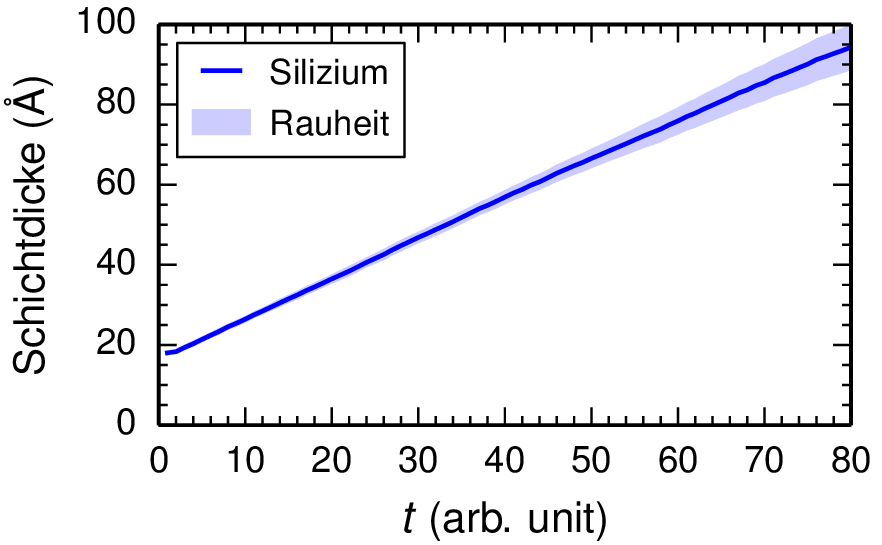
\includegraphics[width=\textwidth]{Si111_combined}
    \subcaption{Dicke und Rauheit der Schicht}
    \label{fig:siliconresults-a}
  \end{subfigure}
  \hfill
  \begin{subfigure}[t]{\subfigwidth}
    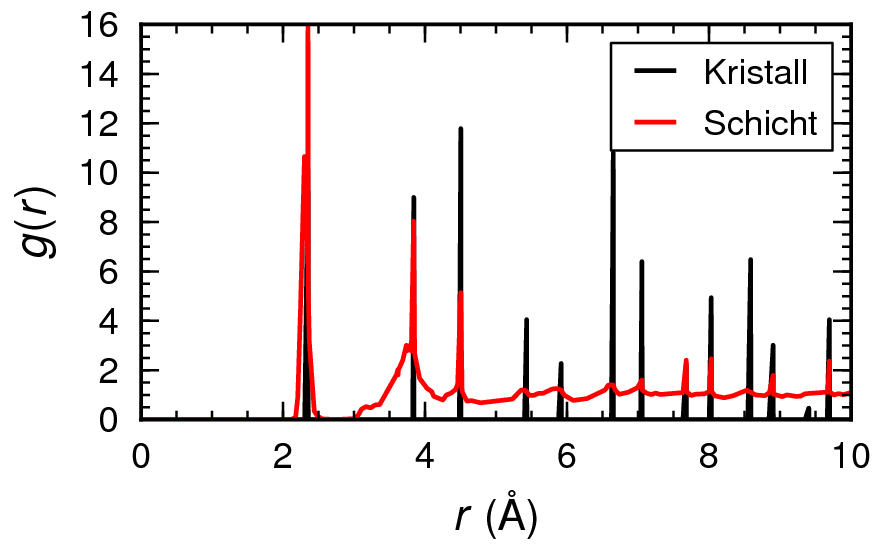
\includegraphics[width=\textwidth]{si111_rdf}
    \subcaption{Radiale Verteilungsfunktion bei $t=80$}
    \label{fig:siliconresults-b}
  \end{subfigure}
  \caption[Struktur einer Silizium-PVD-Schicht aus Parsivald]{
    Struktur einer Silizium-PVD-Schicht aus Parsivald (\SI{10x10}{\nano\meter})
  }
  \label{fig:siliconresults}
\end{figure}

Abbildung~\ref{fig:siliconprofile} stellt die räumliche Verteilung der Unebenheiten dar, die sich lokal in Kratern und Poren von bis zu \SI{32}{\angstrom} Tiefe konzentrieren, aufgrund ihrer geringen Breite aber nur zu einer RMS-Rauheit von \SI{11.5}{\angstrom} führen.
Breitere Krater haben sich durch die geringe Größe des Simulationsraumes nicht entwickelt, jedoch wäre eine Untersuchung einer ca. \SI{500x500}{\angstrom} breiten Struktur auf deren Bildung interessant.
Anhand des Profiles lässt sich auch erkennen, dass mitunter längere Relaxationszeiten oder höhere Teilchenenergien notwendig wären, um Porenbildung weiter zu verringern und langreichweitigere Unebenheiten zu befördern, wie sie etwa bei der Bildung nanoskopischer Silizium-Partikel auftreten würden.

Zum Vergleich beinhaltet Abbildung~\ref{fig:siliconunderrelaxedprofile} das Oberflächenprofil einer unterrelaxierten Oberfläche, wie sie während der Anpassung der Parsivald-Parameter entstanden sind.
Es zeigen sich stärkere Unterschiede und steilere Hänge, die sich aus der hohen Porösität des Materiales ergeben.
Die Porentiefen betragen \SI{6}{\nano\meter} und wachsen linear mit der Schichtdicke, wobei sich aus Zählung der Atome und des Volumens eine Dichte von \SI{2.634}{\gpcc} ergibt, welche durch die Unterschätzung der mittleren Höhe der Oberfläche durch die Nanoporen etwas überschätzt wird und somit oberhalb der kristallinen Dichte von \SI{2.32}{\gpcc} liegt.
Somit ist zu erwarten, dass die Rauheit der Schicht mit stärkerer Relaxierung während der Abscheidung weiter abnimmt.

\begin{figure}[H]
  \centering
  \captionsetup[subfigure]{singlelinecheck=false}
  \begin{subfigure}[t]{7.1cm}
    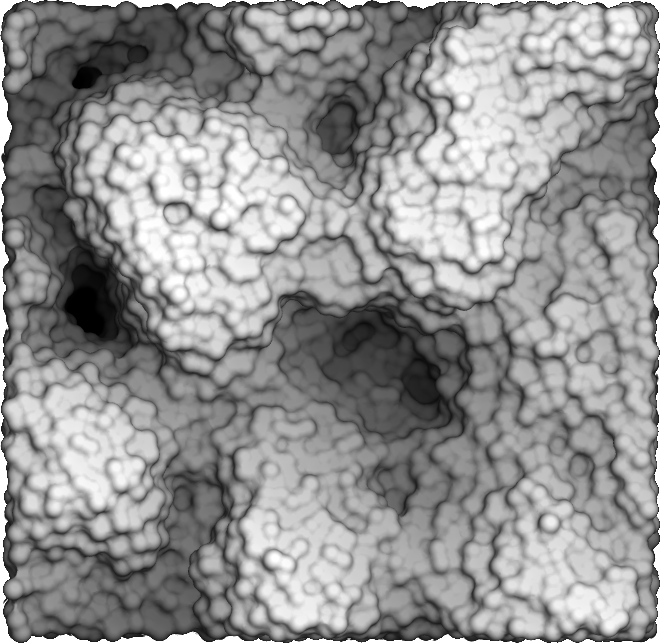
\includegraphics[width=\textwidth]{si111_surface_profile}
  \end{subfigure}
  \begin{subfigure}[t]{1.7cm}
    \def\svgwidth{\textwidth}
    \begin{overpic}[width=0.7cm]{greyhalfscale}
      \put(0,0){\input{img/si111_surface_profile_halfscale.pdf_tex}}
    \end{overpic}
  \end{subfigure}
  \caption[Oberflächenprofil einer Silizium-PVD-Schicht]{
    Oberflächenprofil einer auf Si-(111) per PVD abgeschiedenen Schicht
  }
  \label{fig:siliconprofile}
\todoline{Längenskala}
\end{figure}

\begin{figure}[H]
  \centering
  \captionsetup[subfigure]{singlelinecheck=false}
  \begin{subfigure}[t]{7.1cm}
    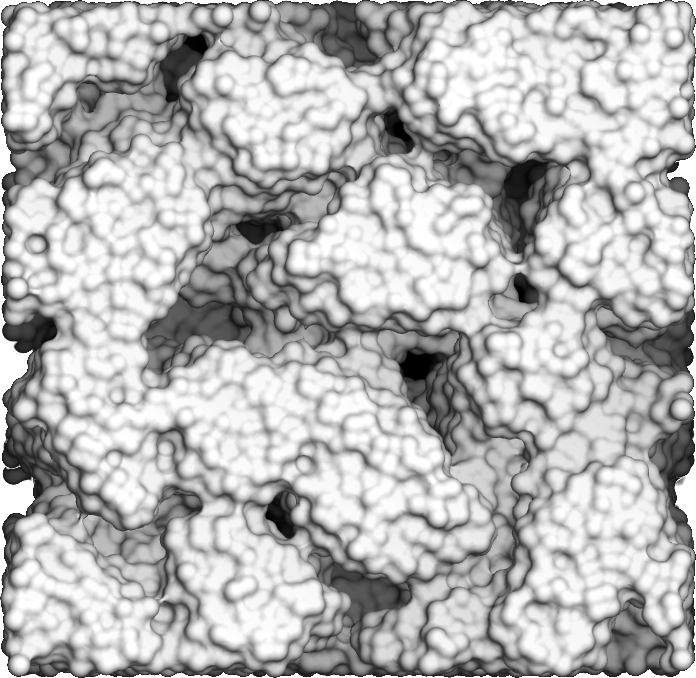
\includegraphics[width=\textwidth]{si111_underrelaxed_profile}
  \end{subfigure}
  \begin{subfigure}[t]{1.7cm}
    \def\svgwidth{\textwidth}
    \begin{overpic}[width=0.66cm]{greyscale}
      \put(0,0){\input{img/si111_underrelaxed_profile_scale.pdf_tex}}
    \end{overpic}
  \end{subfigure}
  \caption[Oberflächenprofil einer unterrelaxierten Siliziumschicht]{
    Oberflächenprofil einer unterrelaxierten, porösen Silizium-PVD-Schicht
  }
  \label{fig:siliconunderrelaxedprofile}
\end{figure}

\subsection{Voruntersuchungen für Siliziumdioxid-CVD}

ReaxFF-Potentiale versprechen die Simulation von Molekülen und deren Reaktion miteinander, die mit den folgenden Tests für Silan und molekularen Sauerstoff überprüft werden sollen.

\subsubsection{Stabilität der Precursormoleküle (\ce{SiH4}, \ce{O2})}

Simulationen einzelner und mehrerer Precursormoleküle (\ce{SiH4} und \ce{O2}) hinsichtlich ihrer Stabilität wurden im mikrokanonischen beziehungsweise kanonischen Ensemble bei verschiedenen Temperaturen durchgeführt.
\todo{Abbildung hier her kopieren}Abbildung~\ref{fig:silanestability} zeigt eine Auswahl der Ergebnisse der Silan-Simulationen, an denen sich erkennen lässt, wie instabile Simulationen zur Ablösung der Wasserstoffatome vom Silanmolekül führen.

\subsubsection{Reaktion der Precursormoleküle (\ce{SiH4 + O2})}

Reaktionen von einzelnen Precursormolekülen wurden stichprobenartig in verschiedenen Orientierungen, Energien und Temperaturen vorgenommen, um einen Überblick über die Verlässlichkeit zu bekommen.
Zusätzlich wurden durchmischte Precursorgase mit dem Ziel eventueller Reaktionen simuliert, was jedoch mit keiner der Parametrisierungen zum gewünschten Erfolg bei hoher Zuverlässigkeit führte.
Einige Parametrisierungen zeigen jedoch vielversprechende Teilreaktionen, die korrekte Doppelbindungen und Bildung von Wasserstoffmolekülen beinhalten (\todo{Abbildung hier her kopieren}Abbildung~\ref{fig:precursorreactions}).
Vor allem bei größeren Reaktionsräumen bilden sich Cluster aus Precursormolekülen, die von attraktiven Termen in den Kraftfeldern dominiert werden, aber nicht durch chemische Wechselwirkungen zu erklären sind (\todo{Abbildung hier her kopieren}Abbildung~\ref{fig:precursorclusters}).


  \clearpage
  \section{Aluminiumoxid-ALD}
\label{aluminaald}

Einen Vorzeige-Prozess für Atomlagenabscheidungen bildet die Abscheidung von Aluminiumoxid \ce{Al2O3}\cite{puurunen_surface_2005}, für die häufig das Precursorpaar Trimethylaluminium (TMA, \ce{Al(CH4)3}) und Wasser genutzt wird.
Mit einer Permittivität von $k\approx 8$ ersetzt Aluminiumoxid gemeinsam mit anderen Materialien langsam Siliziumdioxid ($k=3.9$) als Dielektrikum in der Halbleiterindustrie.
Deshalb soll der TMA-\ce{H2O}-Prozess im Folgenden besonders hinsichtlich der Reaktion der Precursormoleküle mit der Oberfläche untersucht werden.
Einige Reaktionen des Wasser-Halbzyklus' konnten dabei erfolgreich simuliert werden, wo hingegen die Simulation des TMA-Halbzyklus' bisher keinen Erfolg zeigte.

\subsection{Parametersätze}

Für die MD-Simulation von \ce{Al2O3} stehen drei Parametrisierungen zur Verfügung, die bereits aus den Untersuchungen der Silizium-Potentiale bekannt sind:\\
\textbf{Al\_AlO\_AlN} aus LAMMPS\cite{plimpton_lammps_2014}, \textbf{liu\_ettringite}\cite{liu_development_2012}, welches nachfolgend nur als \textbf{liu} geführt werden soll, und \textbf{narayanan}\cite{narayanan_reactive_2012}.
Ihnen ist gemein, dass sie ausgehend von Silizium-kompatiblen Potentialen um Parameter für Aluminium-Verbindungen erweitert wurden.
Auf eine Bewahrung der Konsistenz der Siliziumparameter wurde scheinbar verzichtet, so dass etwa mit der Liu-Datei eine verlässliche Simulation von  Silizium-Verbindungen verhindert, im Gegenzug aber die Simulation von Aluminium-Verbindungen ermöglicht wird.

Die Al\_AlO\_AlN-Datei stammt direkt aus der offiziellen LAMMPS-Distribution, wurde jedoch am 17. Mai 2013 nahezu kommentarlos aus dem Paket entfernt, was sich vermutlich auf mangelnde Kenntnis der Urheberschaft der Parameter sowie ihrer Zielsetzung zurückführen lässt.
Diese Vermutung wird von der Überarbeitung der Referenzen auf wissenschaftliche Publikationen für alle Parametersätze im selben Zeitraum gestützt.
Bei den Recherchen konnte kein Hinweis auf das ursprüngliche Anwendungsgebiet gefunden werden, weshalb mit diesen Parametern berechnete Eigenschaften gesondert überprüft werden sollten.
Es lässt sich jedoch sagen, dass es zeitgleich mit dem \textbf{lg}-Kraftfeld, welches sich bei den Silizium-Untersuchungen als unzureichend heraus gestellt hat, Eingang in LAMMPS gefunden hat.

Das Anwendungsgebiet der Liu-Potentialdatei liegt in der Simulation von Ettringit (\ce{Ca6[Al(OH)6]2(SO4)3 26H2O}), welches \ce{Al-O}-Bindungen und \ce{OH}-Gruppen enthält, so dass zumindest die Simulation des Bulkmateriales und einer hydroxylierten Oberfläche aussichtsreich erscheint.
Sie unterstützt einige der Precursorreaktionen und stellt sich daher als Favorit für Parsivald-Simulationen heraus, obwohl ihr eigentliches Anwendungsgebiet auf strukturellen Eigenschaften von Kristallen liegt.

Zuletzt steht die Narayanan-Parametrisierung für \ce{Li-Al}-Silikate für die Simulation von Eukryptit (\ce{LiAl[SiO4]}) zur Verfügung, lässt aber keine endgültige Aussage über die Qualität der \ce{Al-O}-Bindungen und \ce{OH}-Gruppen zu.
Zwar besteht ihr Trainingssatz aus verschiedenen Lithium-Aluminium-Kristallen, aber nur $\gamma$-\ce{LiAlO2} beinhaltet direkte \ce{Al-O}-Bindungen, wo hingegen keine der Strukturen Wasserstoff beinhaltet.
Es ist daher unwahrscheinlich, dass die Narayanan-Potentialdatei komplizierte Systeme verlässlich darstellt.

Abschließend lässt sich sagen, dass zur vollständigen Simulation der untersuchten Systeme die Erstellung einer eigenen Parametrisierung notwendig wäre, die jedoch den Fokus dieser Arbeit übersteigt.

\subsection{Voruntersuchungen}

Wie in den vorherigen Abschnitten werden hier separate Voruntersuchungen durchgeführt, zu denen die Reaktion von Precursormolekülen mit der Oberfläche ergänzt wurde.

\subsubsection{Strukturelle Eigenschaften von \ce{Al2O3}}

Zum Vergleich der strukturellen Eigenschaften des Bulkmateriales, wie etwa Dichte, Bindungslänge und Koordinationszahlen, wurde ein $\alpha$-\ce{Al2O3}-Kristall bei \SI{1500}{\kelvin} relaxiert und vor den abschließenden Messungen auf Raumtemperatur herunter gekühlt.
Durch einen methodischen Fehler wurden die Systeme zur Dichtebestimmung nicht vollends herunter gekühlt, weshalb die Referenzwerte anhand der Relaxationstemperatur korrigiert wurden.
Damit ergibt sich ein korrigierter Referenzwert zwischen \SI{3.95}{\gpcc} bei \SI{300}{\kelvin} und \SI{3.8}{\gpcc} bei \SI{1500}{\kelvin}\cite{fiquet_high-temperature_1999}, der im direkten Vergleich als \SI{3.85}{\gpcc} abgeschätzt wird.
Der dadurch entstehende Fehler ist im Vergleich zu Abweichungen um \SI{0.5}{\gpcc} gering.

Für die Bestimmung der Dichte der amorphen Struktur wurde das Bulkmaterial über den Schmelzpunkt von \SI{2317}{\kelvin} auf \SI{2555}{\kelvin} erhitzt, auf dieser Temperatur relaxiert und langsam auf Raumtemperatur abgekühlt.
Aufgrund der strukturellen Vielfalt bei amorphen Aluminiumoxiden lässt sich keine eindeutige Referenzdichte angeben, so dass auf den in diesem Zusammenhang häufig genannten Wertebereich von \SIrange{3.2}{3.6}{\gpcc} zurückgegriffen wurde.

Bindungslängen und Koordinationszahlen wurden direkt aus der radialen Verteilungsfunktion bestimmt, wobei die Referenzwerte auf gleiche Weise durch die Untersuchung der Kristallstruktur bestimmt wurden, welche mittels Materials Studio auf Basis eines $\alpha$-\ce{Al2O3}-Kristalles präpariert wurde.

\begin{table}
  \caption[Vergleich struktureller Eigenschaften von Bulk-\ce{Al2O3} mit verschiedenen Parametersätzen]{
    Vergleich struktureller Eigenschaften von Bulk-\ce{Al2O3} mit verschiedenen Parametersätzen.
    Bindungslängen und Koordinationszahlen stammen von einer relaxierten Kristallstruktur.
  }
  \label{tab:aluminabulks}

  \begin{tabularx}{\textwidth}{|Xllll|}
    \hline
    \textbf{Eigenschaft}    & \textbf{Referenz}    & \textbf{Al\_AlO\_AlN} & \textbf{liu}         & \textbf{narayanan}   \\
    \hline
    Dichte, amorph          & \SI{>3.2}{\gpcc}     & ~                     & \SI{3.66}{\gpcc}     & ~                    \\
    Dichte, kristallin      & \SI{3.85}{\gpcc}     & \SI{4.31}{\gpcc}      & \SI{3.88}{\gpcc}     & \SI{3.76}{\gpcc}     \\
    \ce{Al-O}-Bindungslänge & \SI{1.90}{\angstrom} & \SI{1.94}{\angstrom}  & \SI{1.88}{\angstrom} & \SI{1.85}{\angstrom} \\
    \ce{Al-O}-Koordination  & \num{4.00}           & \num{5.40}            & \num{4.55}           & \num{4.05}           \\
    \ce{Al-Al}-Koordination & \num{4.00}           & \num{6.66}            & \num{5.98}           & \num{5.10}           \\
    \ce{O-O}-Koordination   & \num{12.0}           & \num{12.4}            & \num{11.0}           & \num{12.2}           \\
    \hline
  \end{tabularx}
\end{table}

Die Ergebnisse dieser Untersuchungen (Tabelle~\ref{tab:aluminabulks}) zeichnen ein vielseitiges Bild.
Einerseits stimmen die Bindungslängen für alle Parametrisierungen auf \SI{2}{\percent} überein, andererseits ergeben sich aber große Unterschiede in der Dichte der Kristalle, die sich nicht mit den Bindungslängen korreliert sind.

So liegt für die Al\_AlO\_AlN-Parameter eine Abweichung um \SI{+12}{\percent} in der Dichte vor, allerdings ist die Bindungslänge um \SI{2}{\percent} erhöht, was für ähnliche Strukturen zu einer Ausdehnung des Kristalles und somit eine Verringerung der Dichte um \SI{6}{\percent} führen müsste.
Erst bei Betrachtung der Koordinationszahlen zeigt sich die Ursache der Abweichung, die mit einer \ce{Al-O}-Koordinationszahl von \num{5.4} (Kristall: \num{4.0}) in einer Verformung des Kristalles liegt.
Da $\alpha$-\ce{Al2O3} mit \SI{3.95}{\gpcc} eigentlich die dichteste Phase bei Normaldruck ist, sollten nur Übergänge zu weniger dichten Konfigurationen wie amorphem Aluminiumoxid oder etwa $\gamma$-\ce{Al2O3} möglich sein, das aufgrund seiner Porösität eine geringere Dichte von etwa \SI{3.67}{\gpcc}\cite{dynys_alpha_1982} aufweist.
Da hier das Gegenteil der Fall ist, wurde die Al\_AlO\_AlN-Parameterdatei in vielen der nachfolgenden Untersuchungen nicht weiter betrachtet.

Die Liu-Parametrisierung weist ebenfalls eine geringe Änderung aller Koordinationszahlen auf, die sich in einer nur minimalen Verringerung der Dichte äußert.
Anhand einer \ce{Al}-{O}-Koordination von \num{4.55} ist ersichtlich, dass die $\alpha$-Phase mit diesem Parametersatz nicht stabil ist und stattdessen scheinbar eine vergleichsweise dichte amorphe Phase angenommen wird.
Für diesen Parametersatz wurde deshalb auch die Dichte eines amorphen Materiales mit \SI{3.66}{\gpcc} bestimmt, die zwar innerhalb des üblicherweise für amorphe Materialien genannten Bereiches von \SIrange{3.2}{3.6}{\gpcc} liegt, ansonsten aber unterhalb der im ersten Schritt bestimmten Dichte liegt, womit eine höhere Porösität denkbar wird.

Zum Schluss zeigt Die Narayanan-Parameterdatei die besten Ergebnisse für kristalline Strukturen, obwohl sowohl die Bindungslänge als auch die Dichte ca. \SI{2}{\percent} unterhalb der jeweiligen Referenzwerte liegen.
Dies ist im Zusammenhang mit dem Fehlen von \ce{Al-O}-Bindungen in den meisten Molekülen des Trainingssatzes eher überraschend, zeigt aber die Orthogonalität der einzelnen ReaxFF-Parameter, da so die Eigenschaften von $\gamma$-\ce{LiAlO2} die \ce{Al-O}-Bindungen dominieren, statt beim Fitting überschrieben zu werden.

\subsubsection{Precursor-Simulationen}

Zur Untersuchung der Stabilität der Precursor wurden diese einzeln präpariert und per LAMMPS mit verschiedenen Kraftfeldern im kanonischen Ensemble simuliert.
Dabei war schnell ersichtlich, dass Trimethylaluminium (TMA) von der Liu- sowie der Narayanan-Parametrisierung in Ermangelung der Ausprägung von \ce{Al-C}-Bindungen praktisch nicht simuliert werden kann.
Die Methylgruppen binden nicht mit dem zentralen Aluminium-Atom, so dass sie sich von diesem mit fortlaufender Simulationszeit linear entfernen.
Einzig mittels des bereits ausgeschlossenen Al\_AlO\_AlN-Parametersatzes lassen sich stabile TMA-Moleküle simulieren.

\todo[inline]{Bilder im Anhang}

Simulationen von Wassermolekülen sind hingegen mit allen Parametrisierungen geglückt, doch wurden keine umfangreicheren Untersuchungen etwa hinsichtlich der Phasenübergänge angestellt.
Anhand des Al\_AlO\_AlN-Parametersatzes wurden auch Reaktionen zwischen TMA und Wasser simuliert, wie sie beispielsweise bei Vermischung der Precursorgase im ALD-Reaktor auftreten können, aber \todo{phrasing}leider ohne Erfolg.
Es zeigt sich, dass die \ce{Al-C}-Bindungen entweder zu stark oder in zu großem Maß von den Methylgruppen abgeschirmt sind.

\subsubsection{Precursor-Oberflächen-Reaktionen}

Anstatt die Precursormoleküle in der Gasphase reagieren zu lassen, werden hier einzelne Wassermoleküle auf eine $\alpha$-\ce{Al2O3}-Kristalloberfläche gebracht, die mit den darauf befindlichen Sauerstoffatomen reagieren und die Oberfläche so hydroxylieren sollen\todo{Ref}.
Zu diesem Zweck wurde ein mehrschichtiges System mit einem kristallinen Substrat und einer Schicht von Wassermolekülen in Gasphase präpariert, wie es in Abbildung~\ref{fig:wateraluminasurface-a} dargestellt ist.
In der Simulation werden die Wassermoleküle mit einer maxwellschen Geschwindigkeit entsprechend \SI{500}{\kelvin} versehen, die Atome an der Unterseite des Substrates fest gehalten und das Berendsen-Thermostat auf den verbleibenden Teil des Substrates angewandt.
Damit handelt es sich zwar streng gesehen nicht mehr um eine Simulation im kanonischen Ensemble, aber man verzichtet auf separate Integratoren für Substrat (NVT) und Wasser (NVE), deren Grenzen bei erfolgreichen Reaktionen ohnehin aufgelöst werden.

\begin{figure}
  \captionsetup[subfigure]{singlelinecheck=false}
  \def\subfigwidth{0.32\textwidth}
  \begin{subfigure}[t]{\subfigwidth}
    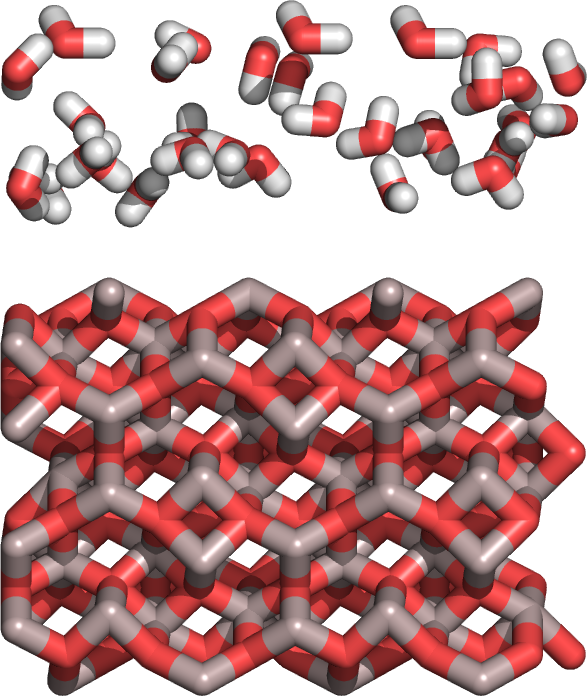
\includegraphics[width=\textwidth]{alumina_h2o_before}
    \subcaption{Seitenansicht, vorher}
    \label{fig:wateraluminasurface-a}
  \end{subfigure}
  \hfill
  \begin{subfigure}[t]{\subfigwidth}
    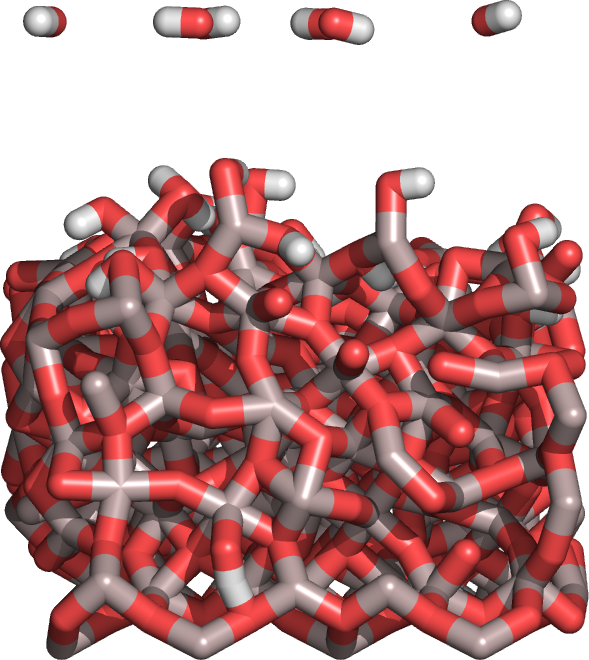
\includegraphics[width=\textwidth]{alumina_h2o_after}
    \subcaption{Seitenansicht, nachher}
    \label{fig:wateraluminasurface-b}
  \end{subfigure}
  \hfill
  \begin{subfigure}[t]{\subfigwidth}
    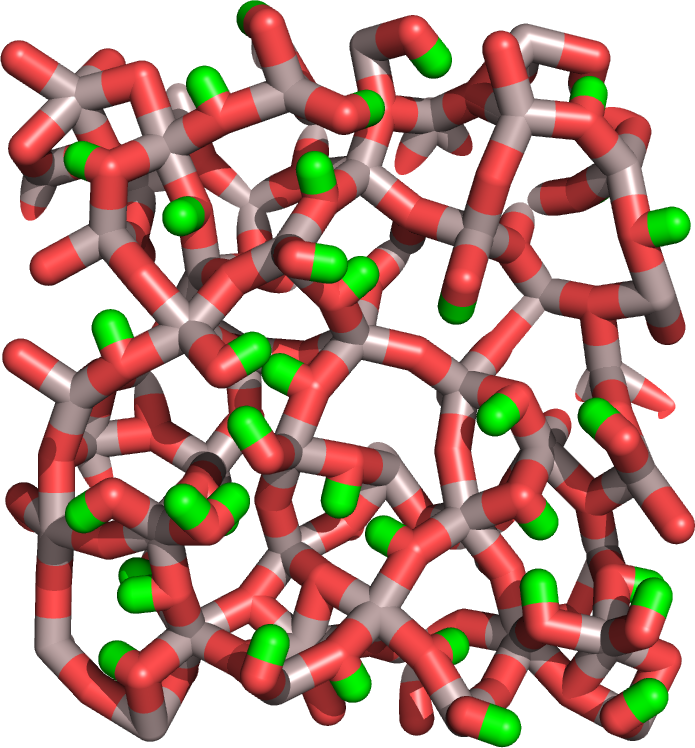
\includegraphics[width=\textwidth]{alumina_h2o_topview}
    \subcaption{Draufsicht, nachher.
      Hydroxyl ist grün hervorgehoben.
    }
    \label{fig:wateraluminasurface-c}
  \end{subfigure}
  \caption[Oberflächenreaktion von Wasser mit $\alpha$-\ce{Al2O3}]{Ergebnisse einer Oberflächenreaktion von Wasser mit $\alpha$-\ce{Al2O3}.
    Das Wasser reagiert mit Sauerstoffatomen an der Oberfläche zu Hydroxylgruppen.
  }
  \label{fig:wateraluminasurface}
\end{figure}

Das Ergebnis der Simulationen für die Liu-Parameter (Abbildungen~\ref{fig:wateraluminasurface-b} und~\ref{fig:wateraluminasurface-c}) zeigt die gleichmäßige Bedeckung der Oberfläche mit Hydroxylgruppen (\SI{9.5}{\per\square\nano\meter}) neben gelegentlich adsorbierten Wassermolekülen, die keine Oberflächenreaktion eingegangen sind.
Letztere sollten aber auf längere Sicht durch die Einflüsse der Überkoordinationsterme des ReaxFF-Potentiales entweder zerfallen oder sich von der Oberfläche lösen.
Trotz unterschiedlicher Startbedingungen stimmt der maximale Bedeckungsgrad der Oberfläche mit Hydroxylgruppen mit aus Elektronenstrukturrechnungen bestimmten Maximalwerten von \SI{9.2}{\per\square\nano\meter}\cite{kim_energy_2011} überein.
Zu Beginn der Simulationen wurden ausreichende Mengen von Wassermolekülen für Bedeckungsgrade von \SI{5.8}{\per\square\nano\meter}, \SI{19.0}{\per\square\nano\meter} und \SI{57.6}{\per\square\nano\meter} präpariert, von denen die überschüssigen Wasser-Moleküle nicht mit der Oberfläche binden, sondern in der Gasphase verbleiben, wie in Abbildung~\ref{fig:wateraluminasurface-b} am oberen Rand des periodischen Simulationsraumes erkennbar ist.
Einige der Wassermoleküle sind durch periodische Randbedingungen des Simulationsraumes zerteilt, weshalb es sich scheinbar um Hydroxylmoleküle handelt, tatsächlich aber komplette Wassermoleküle verbleiben.
Es zeigt sich also die sterische Hinderung der Wasserstoffmoleküle gegenüber weiteren Reaktionen von Wasser mit der Oberfläche.

Eine repulsive Kraft zwischen den Wassermolekülen und der Oberfläche verhindert diese Reaktionen unter Nutzung der Narayanan-Parameter.
Das deutet darauf hin, dass Hydroxylgruppen auf einer Aluminiumoxid-Oberfläche energetisch nicht bevorzugt werden oder die Reaktion mit einer hohen Reaktionsbarriere verbunden ist.
Zusammen mit dem Problem, Trimethylaluminium nicht darstellen zu können, ist dieser Parametersatz somit nicht in der Lage, den ALD-Prozess darzustellen.

\todo[inline]{Hinweis auf vollständige ALD-Simulationen?}
\todo[inline]{Welche der alten Ergebnisse finden hier Anwendung?}

\fi

\cleardoublepage
\chapter{Zusammenfassung und Ausblick}
\label{summary}

\todo{Jörg}

\section{Zusammenfassung}
%% {Was hab ich getan? - Parsivald}

Im Rahmen dieser Arbeit wurde ein bestehendes Hybrid-Modell zur atomistischen Simulation von Atomlagenabscheidungen mit Methoden der Molekulardynamik und der Kinetischen Monte Carlo-Simulationen um die Beschreibung allgemeiner Gasphasenabscheidungen sowie um die Möglichkeit der Nutzung reaktiver Kraftfelder erweitert.
Als Resultat entstand eine Software namens Parsivald, mit der die atomistische Simulation von Gasphasenabscheidungen auf der Größenordnung kompletter Nano-Bauelemente bis zu \SI{1x1}{\micro\meter} ermöglicht wird, was bis zu \num{1e9} Atomen entspricht.
Dies wird durch Nutzung effizienter Datenstrukturen und einem Host-Worker-Schema der Parallelisierung ermöglicht.

%% {Ergebnisse Skalierung}

Anhand der Simulation eines Gold-PVD-Prozesses wurde das Skalierungsverhalten von Parsivald untersucht, wobei gezeigt werden konnte, dass Oberflächen bis zu \SI{0.1x0.1}{\micro\meter} effizient parallelisiert werden können.
Für sie ergibt sich ein linearer Speedup bis zu einer substrat- und potentialabhängigen kritischen Ereignisdichte, bei der auf bis zu \SI{40}{\percent} der Oberfläche gleichzeitig Ereignisse berechnet werden.
Bei Abscheidungssimulationen mit Schichtdicken von \SI{92}{\angstrom} ergibt das ohne spezielle Optimierungen eine Laufzeit von vier Tagen unter Nutzung von durchschnittlich \num{76} parallelen Prozessen.
Für größere Simulationsräume begrenzt der maximale Ereignisdurchsatz des seriellen Hauptprozesses die Zahl der gleichzeitigen Ereignisse, so dass die Parallelisierbarkeit zwar bei \SI{99.5}{\percent} liegt, allerdings nur in \SI{0.06}{\percent} des Simulationsraumes gleichzeitig Ereignisse berechnet werden.
Derart große Simulationsräume stellen ohnehin einen Ausnahmefall dar, für den mehrere tausend Prozessorkerne für eine effiziente Simulation notwendig sind.
Der längste realistische Anwendungsfall war bisher eine Simulation von Silizium-PVD mit reaktiven Kraftfeldern, die ohne weitere Optimierungen drei Wochen Rechenzeit für eine Schicht der Größe \SI{200x200x80}{\angstrom} beanspruchte.
Somit ergibt sich auch unter Nutzung rechenaufwendiger Kraftfelder ein wertvolles Werkzeug zur effizienten Simulation von großflächigen Gasphasenabscheidungen.

%% {Was hab ich getan? - PVD}

Das Parsivald-Modell wurde weiterhin für Simulationen physikalischer Gasphasenabscheidungen von Gold, Kupfer, Silizium und einem Kupfer-Nickel-Multilagensystem mit experimentellen Daten genutzt, deren Ergebnisse mit denen anderer Simulationsmethoden sowie experimentellen Daten verglichen wurden.

Für Gold-PVD zeigt sich dabei epitaktisches Wachstum auf monokristallinen Substraten, das keine Bildung von Nanopartikeln zeigt, wie sie im Experiment durch AFM-Untersuchungen zu beobachten sind.
Dieses Verhalten ist auf Finite-Size-Effekte zurückzuführen, die ein glattes Wachstum der abgeschiedenen Schichten befördern, welches zudem nanoskopische Unebenheiten automatisch ausgleicht und somit Rauheiten von nur \SI{1.2}{\angstrom} erzeugt, verglichen mit experimentellen Werten von \SI{11}{\angstrom}.
Weiterhin ergaben auch Abscheidungssimulationen auf strukturierten Substraten epitaktisches Wachstum, doch formten sich zudem Nanoporen an groben Unebenheiten der Struktur, welche die Oberflächenrauheit dominierten, sich jedoch im Laufe der Simulation langsam schlossen und so Hohlräume innerhalb der Schicht bildeten.
Darin zeigt sich eine Schwäche des Parsivald-Programmes in der Bestimmung der Oberfläche und der damit verbundenen Ereignisorte, die für eine künstliche Abschirmung von Bereichen an steilen Hängen sorgen kann.
Somit sind weitere Anpassungen für die Darstellung beliebiger Auftreffwinkel notwendig, wie sie etwa bei CVD- und ALD-Prozessen vorkommen.


Für die Simulation von Kupfer-PVD war zunächst ein Vergleich verschiedener EAM-Para\-metri\-sierungen notwendig, zwischen denen sich aber keine signifikanten Unterschiede ergaben.
Die anschließenden Abscheidungssimulationen zeigen ebenfalls epitaktisches Wachstum, doch bilden sich in einigen Simulationen kraterförmige Vertiefungen mit einer Breite von \SI{3}{\angstrom} bis \SI{5}{\angstrom}, welche sich mit weiterem Wachstum der Schicht verjüngen und schließlich zu einem kleinen Hohlraum abschließen.
Obwohl derartige Hohlräume in der Realität nicht ausgeschlossen sind, wären sie mit Gitterdefekten verbunden, die in den untersuchten Strukturen nicht vorhanden waren.
Damit ist zu vermuten, dass sich die Vertiefungen als Artefakt der Parsivald-Methode ergeben, welche aber durch weitere Optimierung der Prozessparameter reduziert werden können, wie sich in Simulationen von Multilagen-Abscheidungen zeigte.

In Abscheidungssimulationen von mehrlagigen Schichten per Kupfer-Nickel-PVD sind perfekte Übereinstimmungen mit molekulardynamischen Simulationen in Rauheit und Struktur zu beobachten, wodurch sich für dieses System eine Abwesenheit von Finite-Size-Effekten aufgrund des Parsivald-Modelles zeigt.
Auch für dünne Lagen mit einer Dicke von nur \SI{1}{\nano\meter} sind klare Lagengrenzen vorhanden, wofür allerdings die Relaxationstemperatur sowie die Auftreffenergie des Sputterteilchens leicht erhöht werden musste.
Der selbe Einfluss der Sputterenergie auf die Lagenqualität wurde jedoch auch im Experiment beobachtet.
Durch Einstellung der Simulationsparameter ließ sich die Bildung kraterförmiger Vertiefungen, wie sie bereits bei Simulationen von Kupfer-PVD zu beobachten war, vollständig eliminieren.

Schließlich wurde die Abscheidung amorpher Schichten anhand von Silizium-PVD mit reaktiven Kraftfeldern simuliert, wobei sich dichte, aber vergleichsweise rauhe Schichten ergaben.
\todo{in Silizium-Kapitel einarbeiten}Reaktive Kraftfelder wurden genutzt, da EAM-Formulierungen und N-Teilchen-Potentiale zur Bildung von Kristallen neigen, die zu untersuchenden amorphen Strukturen hingegen auf Valenzbindungen und damit verbundenen Koordinationen basieren, welche von reaktiven Kraftfeldern modelliert werden.
Die  Oberfläche der Schicht zeigt eine RMS-Rauheit von \SI{11.5}{\angstrom}, welche sich mit experimentellen Werten deckt, allerdings im untersuchten Zeitraum \todo{untersuchen, wenn Zeit bleibt}linear ansteigt.
Anhand der Oberflächenprofile ist Porenbildung als Ursache der Rauheit erkennbar, die sich mit erhöhter Relaxationszeit und -temperatur jedoch reduzieren lässt.
Mit fortschreitender Simulationszeit ist eine Schließung der Poren wie bei den kraterförmigen Vertiefungen der Kupfer-PVD-Simulationen zu erwarten, wodurch die Rauheit begrenzt wäre.

%% {Was hab ich getan? - CVD und ALD}

Die betrachteten Silizium-Kraftfelder wurden weiterhin hinsichtlich der Beschreibung der an Siliziumdioxid-CVD beteiligten Precursor-Reaktionen untersucht.
Dabei zeigt sich, dass chemische Reaktionen zwar beschrieben werden, aber mit den untersuchten Kraftfeldern und den genutzten Methoden nicht zuverlässig für Parsivald-Simulationen genutzt werden können.
So sind Reaktionen zwischen Silan und Sauerstoff in der Gasphase nur mit einer begrenzten Menge von Startbedingungen erfolgreich, während sich bei großen Mengen dieser Moleküle Clusterbildung mit unphysikalischen Bindungsarten zeigt.

Für Oberflächen-Reaktionen von Wasser mit Aluminiumoxid kann jedoch eine perfekte Hydroxylierung beobachtet werden, die gute Übereinstimmung der Hydroxyl-Bedeckung mit experimentellen Werten zeigt.
Allerdings konnte der zweite Precursor der \ce{Al2O3}-ALD, Trimethylaluminium, mangels stabiler \ce{Al-C}-Bindungen nicht von den untersuchten ReaxFF-Parametrisierungen beschrieben werden.
Damit war eine reaktive Abscheidungssimulation dieses ALD-Prozesses mit den vorgestellten Methoden bisher nicht erfolgreich.

\section{Ausblick}
%% {Was kann ich tun? - konkrete Untersuchungen}
Anknüpfungspunkte an die Arbeit bestehen in der Optimierung der präsentierten Simulationen zur realistischeren Beschreibung der Strukturen, der Simulation weiterer Abscheidungsprozesse sowie in der Erweiterung von Parsivald um effizientere Algorithmen und Methoden, um die Laufzeit von Abscheidungssimulationen weiter zu senken, wodurch kürzere Iterationszyklen der Prozesspräparation möglich werden.

%% Weitere Optimierungen und Prozesse
Für die EAM-Simulationen lässt sich der Einfluss polykristalliner Substrate auf die Struktur der abgeschiedenen Schicht untersuchen.
Dabei stellt sich die Frage, wie sich die Simulationsparameter im Vergleich zu monokristallinen Substraten und dem damit verbundenen epitaktischen Wachstumsmodus verhalten, um glatte Schichten zu erzeugen.

Gezielte Epitaxie-Simulationen können weiterhin Hinweise auf die Einflüsse der Simulationsparameter und der Finite-Size-Effekte geben, anhand derer Rückschlüsse für die Simulationsparameter allgemeiner Gasphasenabscheidungen gezogen werden können.

Die Simulation von verspannten Multilagen-Systemen, bei denen durch unterschiedliche Gitterkonstanten ein Gitterversatz zu beobachten ist, führt zu der Frage, inwiefern Parsivald den untersuchten Systemen eine kristalline Struktur aufzwingt.

Durch Optimierung der Simulationsparameter für die Simulation der Abscheidung amorpher Schichten lässt deren Einfluss auf die Struktur der Schicht untersuchen.
Ein direkter Vergleich mit rein molekulardynamischen Simulationen ist dafür ebenfalls notwendig, hätte allerdings aufgrund der rechenaufwendigen Potentiale den zeitlichen Rahmen dieser Arbeit gesprengt.

Weitere Untersuchungen der reaktiven Kraftfelder zum Zweck der Beschreibung chemischer Gasphasenabscheidungen führen zu der Frage, wie verlässlich diese zur Simulation der chemischen Reaktionen in CVD-Simulationen genutzt werden können.
Die Nutzung von Energieminimierungen und Metropolis Monte Carlo-Methoden im Gegensatz zur Zeitintegration im kanonischen Ensemble sowie die vorherige Abschätzung des Zielzustandes im KMC-Teil des Modelles können hierbei helfen, die Verlässlichkeit zu erhöhen sowie die notwendige Simulationszeit zu reduzieren.
Andere Gruppen haben bereits ähnliche Modelle erforscht, allerdings dabei aber entweder auf Gitteransätze zurück gegriffen\cite{stamatakis_graph-theoretical_2011} oder nur einatomige epitaktische Systeme untersucht\cite{clark_hybrid_1996}.

%% konkrete Vorschläge zu gemischten Systemen
Die Simulation der Abscheidung gemischter Schichten wie Oxiden und Nitriden ist unter Nutzung reaktiver Kraftfelder auch ohne explizite Beschreibung der Reaktionen hinsichtlich der Frage interessant, inwiefern diese zur Bildung von gleichatomigen Clustern und Überkoordinationen neigen, wie wie bereits für EAM-Potentiale beobachtet werden konnten\cite{lorenz_entwicklung_2012}.
Dabei bieten sich unter anderem \ce{TaN}, welches als Diffusionsbarriere für Kupfer fungiert, und \ce{TiO2}, das als High-$\kappa$-Dielektrikum für Feldeffekt-Transistoren interessant ist, an.
In allen Fällen ist zur Vermeidung der Clusterbildung und zur Bewahrung der Stöchiometrie und Koordinationen eine sorgfältige Untersuchung der Parametrisierungen unerlässlich, weshalb die Präparation dieser Abscheidungssimulationen den Rahmen dieser Arbeit gesprengt hätten.

Zuletzt soll die Simulation des anfänglichen Schichtwachstums auf andersartigen Substraten erwähnt werden.
Zwar wurde mit Kupfer-Nickel-Multilagen-PVD bereits eine solche Untersuchung durchgeführt, doch zeigen diese Materialien gute Hafteigenschaften.
Interessant wäre besonders das Wachstum von High-$\kappa$-Dielektrika auf Silizium und Siliziumdioxid, wie es bei der Produktion moderner MOSFETs auftritt.
Hierbei ist auf Diffusion der Atome auf der Oberfläche und in sie hinein zu beachten, sowie der Wachstumsmodus, der häufig Inselwachstum zeigt und somit mit dr aktuellen Parsivald-Implementierung zu oben beschriebenen nanoporösen Simulationsartefakten führen kann.
%% Parsivald-Erweiterungen

\vspace{0.5em}

Das Parsivald-Modell lässt sich schließlich mit Algorithmen und Methoden erweitern, um so die beobachteten Unzulänglichkeiten zu umgehen, effizientere Simulationen zu erlauben und damit weitere Abscheidungsprozesse mit schnelleren Präparationszyklen zu beschreiben.

So lässt sich der Ereignisdurchsatz des Hauptprozesses verringern, indem einige Vor- und Nachbereitungen in die Worker-Prozesse verlagert werden, wodurch die obere Grenze der Zahl paralleler Worker praktisch eliminiert werden sollte.
Dazu sollte die Host-\-Worker-\-Kom\-mu\-ni\-ka\-tion indirekt über den Management-Prozess des Workerpools laufen, welcher durch eine sorgfältige Überwachung des Workerzustandes unnötige Neuberechnungen unzulässiger Zustände vermeiden könnte.
Eine Parallelisierung des Hauptprozesses ist ebenso denkbar, wird jedoch von den derzeitigen räumlichen Datenstrukturen nicht unterstützt.

Die Abkehr von globalen Datenstrukturen hin zu einer Delaunay-Triangulation des gesamten Raumes brächte neben einer Parallelisierbarkeit des Hauptprozesses auch eine eine implizite Beschreibung der Oberflächenatome per Alpha-Form, womit die Suche bei der Erstellung von Ereignissen massiv beschleunigt würde.
Zusätzlich erlaubt diese Oberflächenbeschreibung beliebige Auftreffwinkel nebst der Ereignisauswahl in bisher abgeschirmten Bereichen, wodurch Verzerrungen der Ereignisraten bei chemische Gasphasenabscheidungen stark reduziert würden.
Außerdem ergeben sich durch die Referenzierung der unmittelbaren Nachbarschaft eines Atomes auch seine Koordinationen sowie potentiellen Bindungen, welche für die Ereignisauswahl hilfreich sind, wodurch eine bisher notwendige Konnektivitätsprüfung jedes Ereignisses entfällt.

Eine der umfangreichsten Ergänzungen bestünde allerdings in der Einführung weiterer atomistischer Optimierungsmethoden, wie etwa Simulated Annealing durch die verbreitete Metropolis Monte Carlo-Methode, die den Rahmen dieser Arbeit gesprengt hätte.

Diese könnten neben molekulardynamischen Potentialen theoretisch auch auf präzisere Methoden wie Elektronenstrukturrechnungen zurück greifen.
Zur Vermeidung unnötiger Redundanz müsste ein selbst-lernendes Verzeichnis der potentiellen Reaktionen eingearbeitet werden, bei Energiebarrieren und damit verbundene Ereignisraten verwaltet und bei Bedarf ergänzt werden.
Diese Methode wird bereits erfolgreich in anderen Off-Lattice-Modellen eingesetzt\cite{biehl_off-lattice_2005,stamatakis_graph-theoretical_2011}.


\cleardoublepage
\begin{appendix}

  \chapter{Physikalische Konstanten und Stoffeigenschaften}
\label{appendix_constants}

\footnotetext[1]{Die Kristall-Bindungslängen wurden über die Kristallstrukturen aus den Gitterkonstanten berechnet}
\footnotetext[2]{Die Dichte bei höheren Temperaturen weit unterhalb des Schmelzpunktes wurde über die Dichte bei Raumtemperatur und den linearen Ausdehnungskoeffizienten berechnet}

\begin{table}[H]
  \centering
  \caption{Physikalische Konstanten}
  \oddrowcolors
  \begin{tabularx}{\textwidth}{|XXR|}
    \hline
    \textbf{Größe}                  & \textbf{Wert}                               & \textbf{Referenz}            \\
    \hline
    Avogadro-Konstante $N_\text{A}$ & \SI{6.02214179e23}{\per\mole}               & \cite{haynes_crc_2011} S.1-1 \\
    Boltzmann-Konstante $k_B$       & \SI{1.3806504e-23}{\joule\per\kelvin}       & \cite{haynes_crc_2011} S.1-2 \\
    Molare Gaskonstante $R$         & \SI{8.314472}{\joule\per\mole\per\kelvin} & \cite{haynes_crc_2011} S.1-2 \\
    Atomare Masseneinheit $u$       & \SI{1.660538782e-27}{\kilo\gram}            & \cite{haynes_crc_2011} S.1-2 \\
    \hline
  \end{tabularx}
\end{table}

\begin{table}[H]
  \centering
  \caption{Eigenschaften von Gold}
  \evenrowcolors
  \begin{tabularx}{\textwidth}{|XXR|}
    \hline
    \textbf{Größe}                           & \textbf{Wert}                                  & \textbf{Referenz}               \\
    \hline
    Dichte $\rho$, \SI{300}{\kelvin}         & \SI{19.3}{\gpcc}                               & \cite{haynes_crc_2011} S.4-65   \\
    Dichte $\rho$, \SI{500}{\kelvin}         & \SI{19.13}{\gpcc}                              & berechnet\footnotemark[2]       \\
    Dichte $\rho_m$, flüssig                 & \SI{17.31}{\gpcc}                              & \cite{haynes_crc_2011} S.4-128  \\
    Linearer Ausdehnungskoeffizient $\alpha$ & \SI{14.2e-6}{\per\kelvin}                      & \cite{haynes_crc_2011} S.12-206 \\
    Schmelztemperatur $T_m$                  & \SI{1064.18}{\celsius} (\SI{1337.33}{\kelvin}) & \cite{haynes_crc_2011} S.4-65   \\
    Atomgewicht $u$                          & \SI{196.967}{\gram\per\mole}                   & \cite{haynes_crc_2011} S.1-12   \\
    Kristallstruktur                         & fcc                                            & \cite{haynes_crc_2011} S.4-147  \\
    Gitterkonstante $a$                      & \SI{4.0786}{\angstrom}                         & \cite{haynes_crc_2011} S.4-147  \\
    Bindungslänge $r_\text{bond}$            & \SI{2.8840}{\angstrom}                         & berechnet\footnotemark[1]       \\
    \hline
  \end{tabularx}
\end{table}

\clearpage

\begin{table}[H]
  \centering
  \caption{Eigenschaften von Kupfer}
  \oddrowcolors
  \begin{tabularx}{\textwidth}{|XXR|}
    \hline
    \textbf{Größe}                           & \textbf{Wert}                                  & \textbf{Referenz}               \\
    \hline
    Dichte $\rho$, fest                      & \SI{8.96}{\gpcc}                               & \cite{haynes_crc_2011} S.4-61   \\
    Dichte $\rho_m$, flüssig                 & \SI{7.997}{\gpcc}                              & \cite{haynes_crc_2011} S.4-128  \\
    Schmelztemperatur $T_m$                  & \SI{1084.62}{\celsius} (\SI{1357.77}{\kelvin}) & \cite{haynes_crc_2011} S.4-61   \\
    Atomgewicht $u$                          & \SI{63.546}{\gram\per\mole}                    & \cite{haynes_crc_2011} S.1-12   \\
    Kristallstruktur                         & fcc                                            & \cite{haynes_crc_2011} S.4-146  \\
    Gitterkonstante $a$                      & \SI{3.6150}{\angstrom}                         & \cite{haynes_crc_2011} S.4-146  \\
    Bindungslänge $r_\text{bond}$            & \SI{2.5562}{\angstrom}                         & berechnet\footnotemark[1]       \\
    Linearer Ausdehnungskoeffizient $\alpha$ & \SI{16.5e-6}{\per\kelvin}                      & \cite{haynes_crc_2011} S.12-206 \\
    \hline
  \end{tabularx}
\end{table}

\begin{table}[H]
  \centering
  \caption{Eigenschaften von Nickel}
  \evenrowcolors
  \begin{tabularx}{\textwidth}{|XXR|}
    \hline
    \textbf{Größe}                & \textbf{Wert}          & \textbf{Referenz}              \\
    \hline
    Kristallstruktur              & fcc                    & \cite{haynes_crc_2011} S.4-150 \\
    Gitterkonstante $a$           & \SI{3.5238}{\angstrom} & \cite{haynes_crc_2011} S.4-150 \\
    Bindungslänge $r_\text{bond}$ & \SI{2.4917}{\angstrom} & berechnet\footnotemark[1]      \\
    \hline
  \end{tabularx}
\end{table}

\begin{table}[H]
  \centering
  \caption{Eigenschaften von Silizium}
  \oddrowcolors
  \begin{tabularx}{\textwidth}{|XXR|}
    \hline
    \textbf{Größe}                & \textbf{Wert}                            & \textbf{Referenz}              \\
    \hline
    Dichte $\rho$, kristallin     & \SI{2.3296}{\gpcc}                       & \cite{haynes_crc_2011} S.4-87  \\
    Dichte $\rho$, amorpher Film  & \SI{2.29}{\gpcc}                         & \cite{remes_optical_1998}      \\
                                  & (\SI{2.2}{\gpcc} - \SI{2.24}{\gpcc})     & \cite{renner_density_1973}     \\
    Schmelztemperatur $T_m$       & \SI{1414}{\celsius} (\SI{1687}{\kelvin}) & \cite{haynes_crc_2011} S.4-87  \\
    Atomgewicht $u$               & \SI{28.086}{\gram\per\mole}              & \cite{haynes_crc_2011} S.4-13  \\
    Kristallstruktur              & diamant                                  & \cite{haynes_crc_2011} S.4-151 \\
    Gitterkonstante $a$           & \SI{5.4305}{\angstrom}                   & \cite{haynes_crc_2011} S.4-151 \\
    Bindungslänge $r_\text{bond}$ & \SI{2.3515}{\angstrom}                   & berechnet\footnotemark[1]      \\
    \hline
  \end{tabularx}

\end{table}

\begin{table}[H]
  \centering
  \caption{Eigenschaften der Silizium-CVD-Precursormoleküle}
  \evenrowcolors
  \begin{tabularx}{\textwidth}{|XXR|}
    \hline
    \textbf{Größe}                                      & \textbf{Wert}          & \textbf{Referenz}             \\
    \hline
    Struktur von Silan $\left(\ce{SiH4}\right)$         & tetraedrisch           & \cite{haynes_crc_2011} S.9-29 \\
    Bindungslänge in \ce{SiH4}                          & \SI{1.4798}{\angstrom} & \cite{haynes_crc_2011} S.9-29 \\
    Bindungslänge von Sauerstoff $\left(\ce{O2}\right)$ & \SI{1.2074}{\angstrom} & \cite{haynes_crc_2011} S.9-26 \\
    \hline
  \end{tabularx}

\end{table}

\begin{table}[H]
  \centering
  \caption{Eigenschaften von Aluminiumoxid}
  \evenrowcolors
  \begin{tabularx}{\textwidth}{|XXR|}
    \hline
    \textbf{Größe}                                         & \textbf{Wert}                            & \textbf{Referenz}                   \\
    \hline
    Dichte $\rho$, $\alpha$-kristallin, \SI{300}{\kelvin}  & \SI{3.99}{\gpcc}                         & \cite{haynes_crc_2011} S.4-45       \\
                                                           & \SI{3.98}{\gpcc}                         & \cite{fiquet_high-temperature_1999} \\
    Dichte $\rho$, $\alpha$-kristallin, \SI{1500}{\kelvin} & \SI{3.80}{\gpcc}                         & \cite{fiquet_high-temperature_1999} \\
    Dichte $\rho$, $\gamma$-kristallin, \SI{300}{\kelvin}  & \SI{3.67}{\gpcc}                         & \cite{dynys_alpha_1982}             \\
    Dichte $\rho$, amorph, \SI{300}{\kelvin}               & \SI{3.2}{\gpcc} - \SI{3.9}{\gpcc}          & \cite{wang_dependence_1997}         \\
    Schmelztemperatur $T_m$, $\alpha$-kristallin           & \SI{2054}{\celsius} (\SI{2327}{\kelvin}) & \cite{haynes_crc_2011} S.4-87       \\
    Atomgewicht $u$, \ce{Al}                               & \SI{26.982}{\gram\per\mole}              & \cite{haynes_crc_2011} S.1-12       \\
    Atomgewicht $u$, \ce{O}                                & \SI{15.999}{\gram\per\mole}              & \cite{haynes_crc_2011} S.1-13       \\
    Kristallstruktur                                       & corundum                                 & \cite{haynes_crc_2011} S.4-146      \\
    Gitterkonstante $a$                                    & \SI{4.7591}{\angstrom}                   & \cite{haynes_crc_2011} S.4-146      \\
    Gitterkonstante $c$                                    & \SI{12.9894}{\angstrom}                  & \cite{haynes_crc_2011} S.4-146      \\
    \hline
  \end{tabularx}

\end{table}

\begin{table}[H]
  \centering
  \caption{Struktur der \ce{Al2O3}-ALD-Precursormoleküle}
  \evenrowcolors
  \begin{tabularx}{\textwidth}{|XXR|}
    \hline
    \textbf{Größe}                                & \textbf{Wert}          & \textbf{Referenz}             \\
    \hline
    Bindungswinkel von Wasser                     & \SI{104.51}{\degree}   & \cite{haynes_crc_2011} S.9-24 \\
    \ce{O-H}-Bindungslänge in Wasser              & \SI{0.9575}{\angstrom} & \cite{haynes_crc_2011} S.9-24 \\
    Struktur von TMA $\left(\ce{Al(CH3)3}\right)$ & trigonal-planar        & \cite{haynes_crc_2011} S.9-46 \\
    \ce{Al-C}-Bindungslänge in TMA                & \SI{1.957}{\angstrom}  & \cite{haynes_crc_2011} S.9-46 \\
    \ce{C-H}-Bindungslänge in TMA                 & \SI{1.113}{\angstrom}  & \cite{haynes_crc_2011} S.9-46 \\
    \hline
  \end{tabularx}
\todoline{Linearen Ausdehnungskoeffizienten rausnehmen, wenn er nirgends benutzt wird. Am Besten nochmal nachfragen}
\end{table}

  \chapter{Datenstrukturen}
\label{appendix_datastructures}

\section{Übersicht über KMC-Operationen}

\begin{table}[h]
  \oddrowcolors
  \caption[Liste der notwendigen Operationen]{
    Übersicht über Operationen, die auf die zugrunde liegenden Datenstrukturen ausgeführt werden.
    Oberflächen- und Bereichssuchen sind am häufigsten.
    %    Zeitkritisch sind die unteren die Bereichs- und Oberflächensuche, da sie für jedes potentielle KMC-Ereignis ausgeführt werden müssen, die anderen nur für jedes versuchte.
  }
  \label{tab:dataops}
  \begin{tabularx}{\textwidth}{|lX|}
    \hline
    \textbf{Operation} & \textbf{Beschreibung} \\
    \hline
    Konstruktion &
    Der einmalige Aufbau aus einer Punktwolke.
    Entspricht oftmals einer einzelnen Einfügung aller Punkte.
    Die Laufzeit ist zweitrangig gegenüber den anderen Operationen
    \\
    Einfügung &
    Ergänzung eines Punktes zu einer bestehenden Struktur.
    Wird nach erfolgten Precursor-Oberflächen-Reaktionen durchgeführt.
    Laufzeiten: \BigO{1} (Listen) bis \BigO{n} (Nachbarschaftslisten)
    \\
    Modifikation &
    Aktualisierung der Position eines Punktes.
    Entspricht gelegentlich einer Entfernung mit anschließender Einfügung.
    Laufzeiten: \BigO{1} (Listen) bis \BigO{n} (Nachbarschaftslisten)
    \\
    Entfernung &
    Entfernung eines Punktes aus der Struktur, entspricht also oft einer inversen Einfügung.
    Wird zur Entfernung von Oberflächen-Liganden aufgerufen.
    Laufzeiten normalerweise wie bei Einfügung
    \\
    Nachbarschaftssuche &
    Extraktion einer Menge von Punkten in der Nähe anderer Punkte, z.B. für kleinere MD-Simulationen.
    Geschieht für jeden Reaktionsversuch.
    Laufzeiten: \BigO{1} (Nachbarschaftslisten) bis \BigO{n} (Listen)
    \\
    Bereichssuche &
    Extraktion einer Menge von Punkten in der Nähe eines beliebigen Punktes, z.B. zur Prüfung möglicher Reaktionen.
    Wird für jede mögliche Reaktion durchgeführt und ist damit häufigste Operation.
    Laufzeiten: \BigO{r_s^3} (Binning) bis \BigO{n} (Listen)
    \\
    Oberflächensuche &
    Die Bestimmung der globalen Oberfläche oder eines Punktes auf der Oberfläche entlang einer Geraden, je nach Prozess und verfügbaren Algorithmen.
    Ist oft der limitierende Faktor der Simulation.
    Delaunay-Triangulationen bilden per Alpha-Form implizit die globale Oberfläche ab, die so direkt in die KMC-Formulierung einfließen kann.
    \\
    \hline
  \end{tabularx}
\end{table}

\section{Beschreibung grundlegender Datenstrukturen}
\todo{einfacher, simpler}
\label{appendix_dataoverview}

\subsection{Atomlisten}

Die Atome des Simulationsraumes werden in einer unsortierten Liste gespeichert, ohne weitere Beziehungen zwischen den Atomen zu speichern.
Damit sind Manipulationsoperationen in konstanter Zeit \BigO{1} möglich, doch müssen Suchoperationen die gesamte Liste der Größe $n$ durchlaufen, wodurch sie für große Systeme durch Laufzeiten von \BigO{n} ungeeignet sind.

\subsection{Nachbarschaftslisten}

Nachbarschaftslisten speichern für jedes Atom eine Referenz auf die Atome in ihrer Nachbarschaft, wodurch Nachbarschaftssuchen effizienter werden, aber jede Manipulation eine Aktualisierung der Nachbarschafts-Referenzen jedes Atomes verursachen.
Die anderen Suchoperationen haben von den Referenzen keine Vorteile und behalten deshalb die Laufzeit von \BigO{n} gegenüber den Atomlisten.
Für MD-Simulationen lohnen sich Nachbarschaftslisten jedoch, da sich die Nachbarschaft nur langsam ändert, aber die meisten Kraftfelder auf eine feste Reichweite begrenzt sind, wodurch mit NB-Listen nur die Kräfte über relevante Atome untersucht werden.

\subsection{Binning-Methoden}
Beim Binning werden Punkte in meist quaderförmige Raumbereiche (Bins) eingeteilt, wodurch bei Suchoperationen vom Zustand der Bins Rückschlüsse auf das Suchergebnis gezogen werden können.
Die Koordinaten des Bins ergibt sich aus der globalen Position der Atome durch lineare Beziehungen.
Innerhalb der Bins liegen wiederum Atomlisten vor, doch werden die Maße der Bins oberhalb der Manipulations-Reichweiten gewählt, so dass die Nachteile der Atomlisten unterdrückt werden.
Bins selbst können in einer übergeordneten Datenstruktur verwaltet werden, beispielsweise die in Abschnitt~\ref{dataoctree} verwendeten Octrees

\subsection{Suchbäume}
In Suchbäumen wird jedes Atom entsprechend seiner Position als Knoten eines balancierten Binär-Baumes verwaltet, so dass Suchoperationen in \BigO{\log{n}} terminieren.
Durch seine Formulierung müssen die Beziehungen zwischen den Knoten rekursiv aktualisiert werden, wofür gelegentlich der gesamte Baum aufwendig umstrukturiert werden muss.
Eine mögliche Form wird mit dem k-d-Baum in Abschnitt~\ref{datakdtree} vorgestellt.

\subsection{Triangulationen}
Triangulationen zerlegen den Simulationsraum raumfüllend in $k$-Simplexe\footnote{Ein $k$-Simplex ist ein Objekt in $k$ Dimensionen mit $k+1$ Eckpunkten, die untereinander mit geraden Kanten verbunden sind.
  Somit ist ein 1-Simplex eine Linie, ein 2-Simplex ein Dreieck, ein 3-Simplex ein Tetraeder, usw.}, an deren Eckpunkten sich die Atome befinden.
Je nach Konstruktionskriterium werden dadurch implizit einige Eigenschaften der Punktwolke dargestellt.
Abschnitt~\ref{datadelaunay} stellt Delaunay-Triangulationen vor, welche durch Beschreibung der Oberfläche der Punktwolke und der Nächstnachbarbeziehungen der Atome schnelle Oberflächen- und Nachbarschaftssuchen auf Kosten der Konstruktion ermöglichen, im Gegensatz zu Suchbäumen aber partitionierbar sind.

\section{Delaunay-Triangulationen}
\label{appendix_delaunay}

\subsubsection{ausgewählte Eigenschaften einer Delaunay-Triangulation}

\begin{itemize}
\item Jeder Punkt ist Eckpunkt eines oder mehrerer Simplexe
\item Simplexe überschneiden sich nicht
\item Im Umkreis eines Simplexes befinden sich keine weiteren Punkte
\item Die Vereinigung aller Simplexe ergibt die konvexe Hülle
\item Alpha-Form $\subset$ Delaunay-Triangulation
\item %Ein Punkt teilt sich mit seinem nächsten Nachbarn mindestens einen Simplex \\
  %$\Leftrightarrow$
  Nächstnachbargraph $\subset$ Delaunay-Triangulation
  %% \item Die Delaunay-Triangulation und das Voronoi-Diagramm über die selben Punkte sind dual\\
  %% $\Rightarrow$ Allgemeine Nachbarschaftssuche ist \BigO{k\log k}
\end{itemize}

\subsection{Algorithmen zur Konstruktion einer Delaunay-Triangulation}

\todo[inline]{mach subsubsections}

Zur Delaunay-Triangulierung aus einer Punktmenge stehen verschiedene Algorithmen zur Verfügung, die auf unterschiedlichen Methoden aufbauen.

\begin{itemize}
\item Flip-basierte Algorithmen (Local Improvement)\\
  Man startet mit einer beliebigen Triangulation, prüft den Umkreis aller Simplexe auf enthaltene Punkte und korrigiert gegebenenfalls per Flip-Algorithmus, der in Abbildung~\ref{fig:delaunay-flip} dargestellt ist.
  Diese Algorithmen konvergieren typischerweise in \BigO{n^2} und sind damit vergleichsweise langsam.

\item Scan-Algorithmus (Incremental Construction)\\
  Man konstruiert schrittweise Simplexe, die das Delaunay-Kriterium erfüllen und keine nachträgliche Änderung benötigen.
  Durch viele Vergleiche und Sortierungen variieren typische asymptotische Laufzeiten zwischen \BigO{n\log{n}} und \BigO{n^2}.

\item Einfügungs-Algorithmen (Incremental Insertion)\\
  Man erstellt einen beliebig großen Simplex, der die gesamte Punktmenge beinhaltet, und fügt schrittweise einzelne Punkte in die Triangulation ein.
  Der den eingefügten Punkt umfassende Simplex wird an ihm in mehrere Unter-Simplexe geteilt, auf den und dessen unmittelbare Nachbarn ein Flip-basierter Algorithmus ausgeführt wird.
  Laufzeiten sind typischerweise gering mit \BigO{n\log{n} + n^{\lceil d/2 \rceil}}.

\item Divide-and-Conquer-Algorithmen\\
  Man teilt die Punktmenge in Untermengen, die rekursiv trianguliert und anschließend an ihren Grenzen miteinander zur Zieltriangulation vereinigt werden.
  Größter Rechenaufwand ist für die Vereinigung der Teiltriangulierungen notwendig, die in zwei Dimensionen aufgrund von Ordnungsrelationen entlang der Grenze beinahe trivial, in höheren Dimensionen jedoch mit Problemen verbunden ist.
  Eine mögliche Lösung ist der DeWall-Algorithmus\cite{cignoni_dewall:_1998}, dessen Methode zur Vereinigung über die Grenzen teilperiodischer Räume interessant wird.
  In zwei Dimensionen erreicht man \BigO{n\log{n}}, höhere Dimensionen können per DeWall-Algorithmus mit einer Laufzeit von \BigO{n^{\lceil d/2 \rceil + 1}} behandelt werden, die sich jedoch nur in pathologischen Fällen zeigt.
  Nimmt man annähernde Gleichverteilungen an, konvergiert dieser Algorithmus in drei Dimensionen subquadratisch, man sollte jedoch betrachten, dass er sich gegenüber anderer Konstruktionsalgorithmen durch einfache Parallelisierung sowie der Möglichkeit der Aktualisierung großer Raumbereiche auszeichnet.

\item Höherdimensionale Einbettung\\
  Hier wird die Punktmenge in eine höhere Dimension transformiert, in der deren konvexe Hülle berechnet wird, die dann in den ursprünglichen Raum herunter projiziert wird und darin eine gültige Delaunay-Triangulation ergibt.
  Dieser Algorithmus ist von rein akademischem Interesse, da Einfügungs-Algorithmen für allgemeine Fälle geringere Laufzeiten ermöglichen.
  Interessant wird diese Methode ebenfalls bei Hinzufügung und Aktualisierung von Punkten.

\end{itemize}

\subsubsection{Flip-Algorithmus}

Basis vieler Algorithmen auf Delaunay-Triangulationen basieren auf dem \textbf{Flip-Verfahren} (Abbildung~\ref{fig:delaunay-flip}), mit dem unzulässige in zulässige Simplexe überführt werden.
Dabei werden Grenzen zu dem benachbarten Simplex, dessen Punkt innerhalb des Umkreises liegt, aufgelöst und aus den dann verfügbaren Punkten zwei neue Simplexe gebildet.
Im Anschluss ist es häufig notwendig, die neu entstandenen Simplexe sowie die ursprünglichen Nachbarn des zweiten Simplexes auf die gleiche Art zu prüfen.

\begin{figure}
  \captionsetup[subfigure]{singlelinecheck=false}{
    \def\subfigwidth{0.23\textwidth}
    \def\svgwidth{\textwidth}
    \begin{subfigure}[t]{\subfigwidth}
      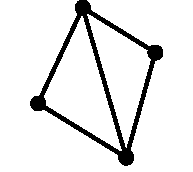
\includegraphics[width=\textwidth]{delaunay-flip-a}
      \subcaption{Ausgangstriangulation}
      \label{fig:delaunay-flip-a}
    \end{subfigure}
    \hfill
    \begin{subfigure}[t]{\subfigwidth}
      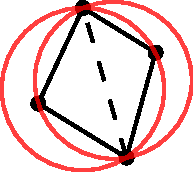
\includegraphics[width=\textwidth]{delaunay-flip-b}
      \subcaption{Vereinigung invalider Simplexe}
      \label{fig:delaunay-flip-b}
    \end{subfigure}
    \hfill
    \begin{subfigure}[t]{\subfigwidth}
      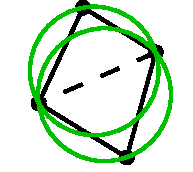
\includegraphics[width=\textwidth]{delaunay-flip-c}
      \subcaption{Aufteilung in neue valide Simplexe}
      \label{fig:delaunay-flip-c}
    \end{subfigure}
    \hfill
    \begin{subfigure}[t]{\subfigwidth}
      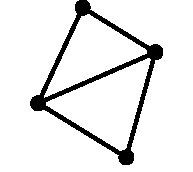
\includegraphics[width=\textwidth]{delaunay-flip-d}
      \subcaption{Ergebnis}
      \label{fig:delaunay-flip-d}
    \end{subfigure}
  }
  \caption[Flip-Algorithmus]{
    Flip-Algorithmus: Invalide Simplexe werden aufgelöst und entlang einer neuen Grenze in neue Simplexe überführt.
    Diese Operation läuft in \BigO{k_d\log{k_d}} Prüfungen bei Aktualisierung der Punkte eines Simplexes, mit $k_d$ als oberer Schranke der Zahl der Simplexe eines Punktes.
  }
  \label{fig:delaunay-flip}
\end{figure}


  \chapter{Ergänzungen zur Laufzeitanalyse von Parsivald}
\label{appendix_runtime}

\section{Einfluss der Ereignis-Laufzeit auf die effiziente Raumgröße\texorpdfstring{$w_\text{eff}$}{weff}}

Die Ereignis-Laufzeit $T_\text{E}$ hat einen ähnlichen Einfluss auf $w_\text{eff}$ wie die MD-Laufzeit $T_\text{MD}$, doch ergibt sich eine inverse Proportionalität $w_\text{eff} \sim T_\text{E}^{-1}$, wie in Abbildung~\ref{fig:weffeventtime} zu erkennen ist.
Dieser Zusammenhang ergibt sich aus dem höheren Ereignisdurchsatz $R_\text{E}$ des Hauptprozesses, mit dem $p_\text{max,2}$ steigt.
Somit verschiebt sich die Grenze $w_\text{eff}$, für die $p_\text{max,1} = p_\text{max,2}$ gilt, weiter nach oben, wodurch größere Räume effizient betrachtet werden können.

\begin{figure}[p]

  \captionsetup[subfigure]{singlelinecheck=false}
  \def\subfigwidth{7cm}
  \begin{subfigure}[t]{\subfigwidth}
    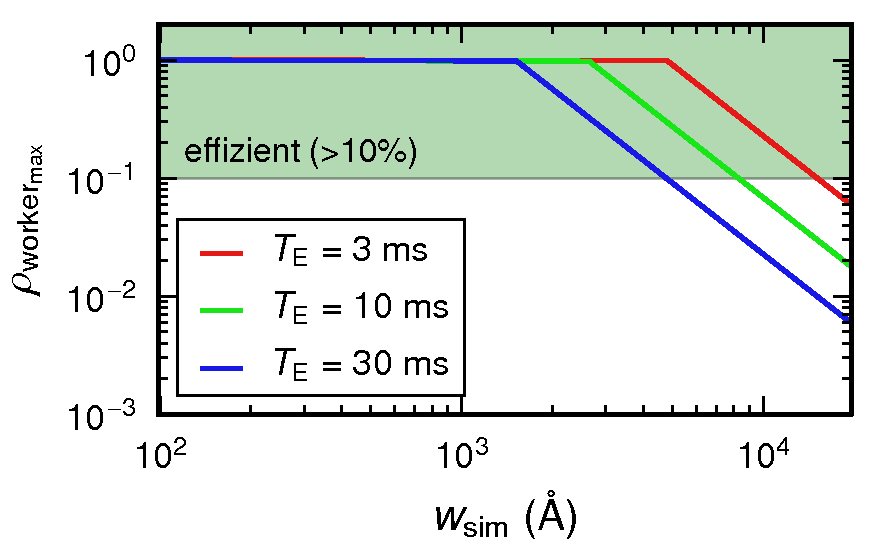
\includegraphics[width=\textwidth]{densitybykmctime}
  \end{subfigure}
  \hfill
  \begin{subfigure}[t]{\subfigwidth}
    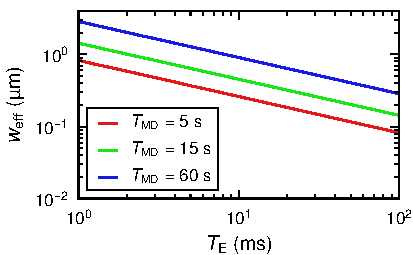
\includegraphics[width=\textwidth]{maxsizebykmctime}
  \end{subfigure}

  \caption{Einfluss der Ereignis-Laufzeit $T_\text{E}$ auf die effiziente Simulationsgröße $w_\text{eff}$}
  \label{fig:weffeventtime}

\end{figure}

\section{Zusätzliche Einflüsse auf das Maximum der Prozesse \texorpdfstring{$p_\text{max}$}{pmax}}

Zusätzlich zur Ereignis- und MD-Laufzeit wird $p_\text{max}$ über die Größe der MD-Boxen $w_\text{MD}$ und die maximale Workerdichte $\rho_\text{worker,max}$ während der Simulation beeinflusst (Abbildung~\ref{fig:pmaxother}).
$\rho_\text{worker}$ ist dabei von der Verteilung der Adsorptionsorte auf der Oberfläche abhängig und hat für gleichverteilte Simulationen von Gold-PVD Werte zwischen \SI{10}{\percent} und \SI{20}{\percent} angenommen.
Für stärker lokalisierte Adsorptionen sind aufgrund der überlappenden MD-Boxen und der daraus resultierenden Abhängigkeit der Ereignisse geringere Werte für $\rho_\text{worker}$ zu erwarten.
Es gilt $w_\text{eff} \sim \rho_\text{worker,max}^{-1}$

Die Erhöhung von $w_\text{MD}$ hat umfangreichere Einflüsse und verursacht eine Verringerung von $\rho_\text{max}$ aufgrund der Größe der Box, sowie eine Erhöhung von $T_\text{MD}$ und $T_\text{E}$ aufgrund der größeren Zahl an Atomen in der Box, was insgesamt zu einer Erhöhung von $w_\text{eff}$ führt.
Somit wird $p_\text{max}$ für $w_\text{sim} < w_\text{eff}$ verringert und für $w_\text{sim} > w_\text{eff}$ erhöht.
Da mit der Vergrößerung der MD-Boxen auch die gesamte Laufzeit nahezu proportional skaliert (Abbildung~\ref{fig:tpother}), wird $w_\text{MD}$ meistens minimal gewählt.

\begin{figure}[p]

  \captionsetup[subfigure]{singlelinecheck=false}
  \def\subfigwidth{7cm}
  \begin{subfigure}[t]{\subfigwidth}
    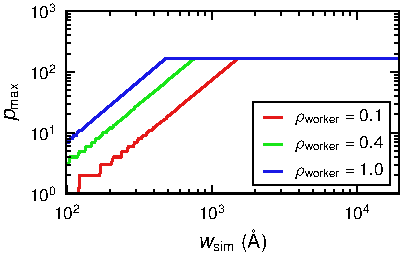
\includegraphics[width=\textwidth]{workersbydensity}
  \end{subfigure}
  \hfill
  \begin{subfigure}[t]{\subfigwidth}
    \includegraphics[width=\textwidth]{workersbymdsize}
  \end{subfigure}

  \caption{Einfluss von $\rho_\text{worker}$ und $w_\text{MD}$ auf das Maximum von Prozessen $p_\text{max}$}
  \label{fig:pmaxother}

\end{figure}

\begin{figure}[p]

  \captionsetup[subfigure]{singlelinecheck=false}
  \def\subfigwidth{7cm}
  \begin{subfigure}[t]{\subfigwidth}
    \includegraphics[width=\textwidth]{runtimebydensity}
  \end{subfigure}
  \hfill
  \begin{subfigure}[t]{\subfigwidth}
    \includegraphics[width=\textwidth]{runtimebymdsize}
  \end{subfigure}

  \caption{Einfluss von $\rho_\text{worker}$ und $w_\text{MD}$ auf die Laufzeit $T_p$}
  \label{fig:tpother}

\end{figure}

\clearpage

\section{Abschätzung der maximalen Workerdichte per Random Sequential Adsorption}
\label{appendix_rsamaxdensity}

Bei Random Sequential Adsorption (RSA) werden geometrische Objekte nichtüberlappend an zufälligen Positionen in einem Raum verteilt, bis kein weiteres Objekt platziert werden kann.
Die Verteilung der quadratischen Worker auf der Oberfläche geschieht auf eine ähnliche Weise, sodass als Grenzwert der Workerdichte \SI{56.2}{\percent}\cite{brosilow_random_1991} angegeben werden kann.

Da Parsivald die Ereignisorte mit KMC-Methoden wählt, muss die zeitliche Reihenfolge der Ereignisse eingehalten werden, weshalb die überdeckenden Ereignisse nicht verworfen werden, sondern bis zum Abschluss des überdeckten Ereignisses zurück gestellt werden und sich so ein kompletter Abhängigkeitsbaum aufbaut, wie er in meiner Bachelorarbeit wird\cite{lorenz_entwicklung_2012}.
Dadurch kollidieren die MD-Boxen zurückgestellter Ereignisse mit nachfolgenden Ereignissen, welche wiederum zurückgestellt werden müssen.
Somit reduziert sich das Maximum der Workerdichte für große Simulationsräume auf den Grenzwert von \SI{25.95}{\percent} (Abbildung~\ref{fig:rsamaxdensity}).
Dieser Wert wurde über eine modifizierte RSA-Simulation ermittelt, die auf diese Parsivald-Methode der Ereignisauswahl und -Durchführung angepasst wurde.

KMC-Ereignisse werden in Parsivald für geringe Zeiträume durch einen trivialen Warte\-schlangen-Algorithmus vorausberechnet, um eine hohe Parallelisierbarkeit zu ermöglichen.
Um häufige Revisionen der Ereignisse und damit verbundene Leistungseinbußen zu vermeiden, wird die Tiefe der Abhängigkeitsbäume der Ereignisse beschränkt, was sich in einer verminderten Zahl von Versuchen zur Erzeugung eines neuen KMC-Ereignisses äußert.
Im Gegenzug sinkt damit die Workerdichte auf die für Gold-PVD und Kupfer-PVD in den Abschnitten~\ref{goldpvd} und~\ref{copperpvd} beobachteten Werte von \SIrange{10}{20}{\percent}.

\vspace{2em}

\begin{figure}[h]
  \centering
  \includegraphics[width=10cm]{rsa_maxdensity}

  \caption[Abschätzung der maximalen Workerdichte per RSA-Simulation]{
    Abschätzung der maximalen Workerdichte durch eine modifizierte RSA-Simulation.
    Als Grenzwert für viele KMC-Versuche ergibt sich \SI{25.95}{\percent}
  }
  \label{fig:rsamaxdensity}

\end{figure}

  %% appendix_lammpsrant
  \chapter{Multilagen-PVD}
\label{appendix:multilayer}

\section{Porenbildung bei Unterrelaxation}

Nach der Adaptierung von Kupfer-Prozess-Parametern auf das Kupfer-Nickel-Multilagensystem konnten Abscheidungen von mehrlagigen Systemen simuliert werden, jedoch haben sich bei diesen verschiedene Defekte gebildet, die im Folgenden vorgestellt werden sollen.

Typischerweise deuten Wachstumsdefekte auf geringe Relaxationszeiten, geringe Sputterenergien oder geringe Temperaturen hin.
Das folgende System wurde bei \SI{500}{\kelvin} mit \SI{5.4}{\electronvolt} Auftreffenergie pro Teilchen für \SI{1.2}{\nano\second} relaxiert.
Die Auftreffenergie wird jedoch hauptsächlich Teil vom Thermostat abgefangen, so dass sie mit \SI{5.4}{\electronvolt} eigentlich zu niedrig liegt.

Als Resultat bilden sich Poren (Abbildung~\ref{fig:multilayer_surfacefail}), die sich vergleichbar zu den Kupferkratern in Abbildung~\ref{fig:coppercrater} entwickeln, sich aber erst spät wieder schließen.

\begin{figure}[h!]
  \centering
  \includegraphics[height=10cm]{CuNi_surface8_noalpha}
  \caption{Oberflächenprofil einer CuNi-Oberfläche nach nur 4 Lagen (\SI{60}{\angstrom})}
  \label{fig:multilayer_surfacefail}
\end{figure}

\clearpage
Abbildung~\ref{fig:multilayer_columnfail} zeigt ein gleichartiges Resultat, das mit denselben Parametern erzeugt wurde.
Hier ist erkennbar, wie sich die gebildeten Poren wieder schließen.
Zur einfacheren Veranschaulichung wurde nur ein wenige Nanometer dünnes Profil abgebildet.

\begin{figure}[h!]
  \captionsetup[subfigure]{singlelinecheck=false}
  \def\subfigwidth{7cm}
  \begin{subfigure}[t]{\subfigwidth}
    \includegraphics[width=\textwidth]{CuNi_thicklayers}
    \caption{Profil einer Schicht mit 6 Lagen je \SI{6}{\nano\meter}}
    \label{fig:multilayer_thickfail}
  \end{subfigure}
  \hfill
  \begin{subfigure}[t]{\subfigwidth}
    \includegraphics[width=\textwidth]{CuNi_columnfail}
    \subcaption{Dünnes Profil nach 24 Lagen (\SI{180}{\angstrom})}
    \label{fig:multilayer_columnfail}
  \end{subfigure}
  \caption{Fehlgeschlagene \ce{CuNi}-Abscheidungen während der Parameter-Optimierung}
\end{figure}

\section{Multilagen mit einer Dicke von 5 nm}

Ergänzend wurden auch Untersuchungen an Schichten mit Lagendicken begonnen, die sich mehr an experimentellen Werten von mehreren Nanometern orientieren.
Abbildung~\ref{fig:multilayer_thickfail} stellt ein solches System dar, das aber aus Mangel an Rechenzeit für die notwendige Optimierung der Simulationsparameter nicht weiter untersucht wurde.
Aus diesem Grund sind auch Krater- und Porenbildungen zu beobachten, die erwartungsgemäß mit Eingabe der optimalen Werte aus Kapitel~\ref{multilayer} eliminiert werden.

  \chapter{Silizium-PVD}
\label{appendix:silicon}

\section{Voruntersuchungen}

Die Bindungslängen für verschiedene Parametrisierungen wurden direkt aus der radialen Verteilungsfunktion für einen Silizium-Kristall ermittelt.
In Abbildung~\ref{fig:sisibondlengths} ergibt sich dabei für die Newsome-Parametrisierung eine zusätzliche RDF-Spitze knapp vor der eigentlichen Bindungslänge, durch welche die eigentliche Bindungslänge unterschätzt wird.
Sie entsteht durch Abspaltung von der Hauptbindungslänge und stellt somit für kristallines Silizium einen Parametrisierungs-Fehler dar.

\begin{figure}[!ht]
  \centering
  \includegraphics[width=10cm]{SiSi_npt_bondlengths}
  \caption{Bindungslängen von c-\ce{Si} für ReaxFF-Parametrisierungen}
  \label{fig:sisibondlengths}
\end{figure}

Die radialen Verteilungsfunktionen des Kulkarni-Potentiales in Abbildung~\ref{fig:kulkarnirdf} zeigen vollständige Übereinstimmung mit der RDF des Kristalles nach thermischer Relaxierung im kanonischen Ensemble.
Im Großkanonischen Ensemble schrumpft der Kristall zwar um \SI{2.1}{\percent}, behält seine Struktur aber ohne weitere Einschränkung bei.
Während der Relaxierung wurde der Kristall auf \SI{500}{\kelvin} erhitzt, wodurch sich die RDF-Spitzen verbreitert und dabei überlagert haben, beim Abkühlen aber wieder zur idealen Kristallstruktur zusammenzogen.

\begin{figure}[!ht]
  \centering
  \includegraphics[width=10cm]{kulkarni_rdf_crystal}
  \caption[Radiale Verteilungsfunktionen von relaxiertem c-\ce{Si}]{
    Radiale Verteilungsfunktionen von relaxiertem c-\ce{Si} mit kulkarni
  }
  \label{fig:kulkarnirdf}
\end{figure}

Bei Relaxierung von amorphem Silizium nach den oben beschriebenen Methoden ist anhand der RDF in Abbildung~\ref{fig:amorphousrdf} keine Kristallisation zu erkennen.
Bereits nach \SI{4}{\angstrom} ist keine langreichweitige Ordnung erkennbar, doch ist die Bindungslänge bei \SI{2.339}{\angstrom} klar erkennbar.
Damit liegt sie ca. \SI{3}{\percent} oberhalb ihrer kristallinen Bindungslänge.
Weitere strukturelle Werte für alle untersuchten Parametrisierungen sind in Tabelle~\ref{tab:amorphoussilicon} zu finden.

\begin{figure}[!ht]
  \centering
  \includegraphics[width=\textwidth]{kulkarni_rdf_amorphous}
  \caption[Radiale Verteilungsfunktionen von relaxiertem a-\ce{Si}]{
    Radiale Verteilungsfunktionen von relaxiertem a-\ce{Si} mit kulkarni
    }
  \label{fig:amorphousrdf}
\end{figure}

\begin{table}[!ht]
  \begin{threeparttable}

    \caption{Vergleich der Struktur amorphen Siliziums}
    \label{tab:amorphoussilicon}

    \oddrowcolors
    \begin{tabularx}{\textwidth}{|llXXlX|}
      \hline
      \textbf{Parametrisierung} & \multicolumn{2}{l}{\textbf{Bindungslänge}} & \textbf{Koord.} & \textbf{Dichte} & ~  \\
      \hline
      (kristallin) & \SI{2.352}{\angstrom} & ~                    & \num{4.00}  & \SI{2.330}{\gpcc} & ~                         \\
      amorph       & ~                     & ~                    & ~           & \SI{2.3}{\gpcc}   & \cite{remes_optical_1998} \\
      Al\_Al0\_AlN & \SI{2.379}{\angstrom} & \SI{+1.15}{\percent} & \num{4.59}  & \SI{2.373}{\gpcc} & \SI{+3.15}{\percent}      \\
      kulkarni     & \SI{2.339}{\angstrom} & \SI{-0.55}{\percent} & \num{4.05}  & \SI{2.361}{\gpcc} & \SI{+2.65}{\percent}      \\
      liu\_ettr.   & \SI{2.401}{\angstrom} & \SI{+2.08}{\percent} & \num{4.10}  & \SI{2.314}{\gpcc} & \SI{+0.61}{\percent}      \\
      narayanan    & \SI{2.383}{\angstrom} & \SI{+1.32}{\percent} & \num{4.05}  & \SI{2.365}{\gpcc} & \SI{+2.83}{\percent}      \\
      newsome      & \SI{2.153}{\angstrom} & \SI{-8.46}{\percent} & \num{1.17}  & \SI{2.398}{\gpcc} & \SI{+4.26}{\percent}      \\
      nielson      & \SI{2.411}{\angstrom} & \SI{+2.51}{\percent} & \num{4.82}  & \SI{2.358}{\gpcc} & \SI{+2.52}{\percent}      \\
      zhang        & \SI{2.357}{\angstrom} & \SI{+0.21}{\percent} & \num{4.39}  & \SI{2.329}{\gpcc} & \SI{+1.26}{\percent}      \\
      \hline
    \end{tabularx}

  \end{threeparttable}
\end{table}

\section{Precursorsimulationen}

Zur Simulation der Stabilität von Silan wurde dieses mit Materials Studio präpariert und anschließend im mikrokanonischen Ensemble mit einer anfänglichen Temperatur von \SIrange{300}{700}{\kelvin} relaxiert.
Eine Strukturoptimierung wurde nicht durchgeführt, da die thermische Stabilität untersucht werden sollte und die untersuchten Moleküle keine komplizierten Strukturen beinhalten.

Bei Al\_Al0\_AlN, Kulkarni, Nielson und Zhang behalten die Silan-Moleküle ihre Struktur, während die einige der \ce{Si-H}-Bindungen bei den anderen Parametrisierungen brechen und einzelne Wasserstoff-Moleküle freigeben (Abbildung~\ref{fig:silanestability}).
Dieser Effekt ist unabhängig von der anfänglichen Temperatur.

Für die Reaktion von Silan mit Wasser wurden beide Moleküle außerhalb der Cutoff-Reichweite der ReaxFF-Potentiale mit zufälligen Orientierungen platziert und zusätzlich zu einer geringen Anfangsgeschwindigkeit zueinander beschleunigt.
Die relativen kinetischen Energien reichen von \SI{0.1}{\electronvolt} bis \SI{10}{\electronvolt} und decken somit einen breiten Geschwindigkeitsbereich ab.

Die meisten Parametrisierungen zeigen keine Änderung des Bindungszustandes der Moleküle, allerdings zeigen Zhang, Newsome und Kulkarni bindendes Verhalten (Abbildung~\ref{fig:precursorreactions}).
Einige der Zhang-Simulationen zeigen, wie in der Abbildung dargestellt, eine Überzahl an stabilen Bindungen, doch lösen sich diese bei höheren Anfangsgeschwindigkeiten.
Die beiden anderen Potentiale zeigen meist die korrekte Zahl an Bindungen für das Silizium-Atom, doch bildet sich meist atomarer Sauer- und Wasserstoff, der allerdings bei Kontakt mit einem anderen Atom Bindungen aufbauen müsste.

Bei der Reaktion mehrer Precursor-Moleküle im kanonischen Ensemble zeigen sich gravierendere Unterschiede (Abbildung~\ref{fig:precursorclusters}).
Kulkarni-Simulationen bilden etwa Sauerstoff-Cluster sowie Bindungen zwischen den Wasserstoff-Atomen der Silan-Moleküle.
Einzig Zhang stellt halbwegs korrekte Bindungen dar, was vermutlich durch die Anwendung zur Beschreibung von Reaktionen vergleichsweise großer Moleküle gegeben ist.
Es zeigen sich jedoch auch hier Überkoordinationen, wie sie bereits in Abbildung~\ref{fig:precursorreactions} beobachtet werden konnten.
Eine Simulation mit Newsome wurde aufgrund der instabilen Silan-Moleküle nicht durchgeführt.

\begin{figure}[!ht]

  \captionsetup[subfigure]{singlelinecheck=false}
  \def\subfigwidth{0.32\textwidth}
  \begin{subfigure}[t]{3.5cm}
    \includegraphics[width=\textwidth]{silane_nielson_stable}
    \subcaption{nielson: stabil}
  \end{subfigure}
  \hfill
  \begin{subfigure}[t]{4.5cm}
    \includegraphics[width=\textwidth]{silane_narayanan_unstable}
    \subcaption{narayanan: instabil}
  \end{subfigure}
  \hfill
  \begin{subfigure}[t]{5cm}
    \includegraphics[width=\textwidth]{silane_liu_unstable}
    \subcaption{liu-ettringite: instabil}
  \end{subfigure}

  \caption[Stabilitätsuntersuchungen von Silan]{
    Stabilitätsuntersuchungen von Silan (\ce{SiH4}) bei 600K (CVD-Temperatur)
  }
  \label{fig:silanestability}

\end{figure}

\begin{figure}[!ht]

  \captionsetup[subfigure]{singlelinecheck=false}
  \def\subfigwidth{0.32\textwidth}
  \begin{subfigure}[t]{3cm}
    \includegraphics[width=\textwidth]{silane_reaction_zhang}
    \subcaption{zhang: Überzahl an Bindungen}
  \end{subfigure}
  \hfill
  \begin{subfigure}[t]{5cm}
    \includegraphics[width=\textwidth]{silane_reaction_newsome}
    \subcaption{newsome: korrekte Stöchiometrie}
  \end{subfigure}
  \hfill
  \begin{subfigure}[t]{4.5cm}
    \includegraphics[width=\textwidth]{silane_reaction_kulkarni}
    \subcaption{kulkarni: Korrekte \ce{Si}-Bindungen, aber \ce{O}-Atom}
  \end{subfigure}

  \caption[Reaktionen von \ce{SiH4} mit \ce{O2}]{
    Reaktion von \ce{SiH4} mit \ce{O2}
  }
  \label{fig:precursorreactions}

\end{figure}

\begin{figure}[!ht]

  \captionsetup[subfigure]{singlelinecheck=false}
  \begin{subfigure}[t]{4cm}
    \includegraphics[width=\textwidth]{oxygen_cluster}
    \subcaption{kulkarni: \ce{O2}-Cluster}
  \end{subfigure}
  \hfill
  \begin{subfigure}[t]{5.5cm}
    \includegraphics[width=\textwidth]{kulkarni_precursor_cluster}
    \subcaption{kulkarni: Precursor-Cluster}
  \end{subfigure}
  \hfill
  \begin{subfigure}[t]{4.5cm}
    \includegraphics[width=\textwidth]{zhang_precursor_cluster}
    \subcaption{zhang: Reaktionen}
  \end{subfigure}

  \caption[Cluster von Precursormolekülen]{Clusterbildung und partielle Reaktionen von Precursormolekülen bei 500K}
  \label{fig:precursorclusters}

\end{figure}

  \chapter{Aluminiumoxid}
\label{appendix_alumina}

\section{Simulationen von Trimethylaluminium}

\todoline{TMA-Simulationen}

\section{Wasser-\ce{Al2O3}-Reaktionen}

\todoline{Bedeckungszahlen}
\todoline{Ergebnis von 02\_water\_surface}



  %\newpage
  %\addcontentsline{toc}{chapter}{B. Danksagung}
  %% \thispagestyle{empty}
  %% \chapter{Danksagung}
  %% \newpage
  %\chapter{}
  %% \null\vfil
  %% \begin{center}
  %%   %\vspace{-.5em}\vspace{\parsep}
  %%   %\vspace{0.2cm}
  %%   \vspace{3cm}
  %% \end{center}
  %% \par\vfil\null
  %\cleardoubleemptypage

\end{appendix}

%\part*{Anhang}


%\manualmark
%\markboth{Literaturverzeichnis}{Literaturverzeichnis}
%\bibliographystyle{bibstyles/gerunsrtmod} % titel kursiv, journal normal; ist fein, modifiziert damit die Namen stimmen
\bibliographystyle{bibstyles/bibelor} % Original von Fabian Teichert

\newcommand{\bstmaxid}{150}
\ifdraft{
  \newcommand{\bstwarn}[1]{\color{red} #1}
}{
  \newcommand{\bstwarn}[1]{\ignore{#1}}
}

\bibliography{literature} %standard

\todoline{dois und links überarbeiten, Patentnummern eintragen, Kramer: Beide Vornamen, Buda: doi!, biehl: ISBN/doi, dwivedi\_2010: doi/isbn, dwivedi\_2009-2: doi nicht verlinkt, gosalvez: doi!, lorenz: link, ylammi: doi nicht verlinkt, ritala: ISBN!, suntola patent: Patentnummer!, Voter: Adresse, seyama: doi nicht verlinkt, higashiwaki: doi nicht verlinkt}
\todoline{doi-links fehlen -> url fehlt, ISBNs: gleiche Formatierung}


%======================================================================
%  Selbstständigkeitserklärung
%======================================================================

%\addcontentsline{toc}{chapter}{C. Selbständigkeitserklärung}
%\chapter{Selbstständigkeitserklärung}
%\includepdf[pagecommand={}]{selbststaendigkeitserklaerung.pdf}
%\stepcounter{page}
%\includepdf{selbststaendigkeitserklaerung.pdf}
\cleardoublepage
\includepdf[pagecommand={\thispagestyle{plain}}]{selbststaendigkeitserklaerung.pdf}


\end{document}

\todoline{Prüfen, ob die Abkürzungen im Text ordentlich eingeführt werden}
\todoline{figures und tables positionieren!}
\todoline{Theorie -> Grundlagen}
\todoline{Erste Absätze: Keine Einrückung.}
\todoline{Überprüfen, wo von Simulationen, Parsivald-Problemen, allgemeines Systemverhalten und Experimenten die Rede ist}
\todoline{Keine Ebenen mit nur einem Eintrag (e.g. Kupfer-Ergebnisse)}
\todoline{Mit Vortrag abgleichen}
\todoline{Aktivierungsenergien, Arrhenius-Gleichung, PVD-Raten einbinden}
\todoline{Inhalte aus dem Anhang in die Arbeit ziehen, insbesondere für Silizium}
\todoline{hier und da eine Längenskala}
